\documentclass[12pt, letterpaper, twoside]{article}

\usepackage{geometry}
\usepackage{graphicx}
\usepackage{amsmath}
\usepackage{amsfonts}
% For bold face mathcal
\DeclareMathAlphabet\mathbfcal{OMS}{cmsy}{b}{n}

\usepackage{tabularx,booktabs}
\usepackage{multirow}
\usepackage{todonotes}
\usepackage{enumitem}

%\usepackage{lipsum}
\usepackage{fancyhdr}
%\usepackage{layout}
\usepackage{lettrine}
\usepackage[explicit]{titlesec}
\usepackage{watermark}
\usepackage{color}
\usepackage[final]{pdfpages}
\usepackage{setspace}

\usepackage[sort, numbers, compress]{natbib}
\bibliographystyle{main} % custom style see README.md for more info
\usepackage[nottoc]{tocbibind}

\usepackage{doi}
\usepackage{hyperref}


\usepackage[demo,abs]{overpic}
\newcommand{\igwithlabel}[3]{\begin{overpic}
  [#2]{#3}
  \put(5,10){\small #1}
\end{overpic}}

\usepackage{caption}
\captionsetup{margin=10pt,font=small,labelfont=bf}

\usepackage{enumitem}
\setlist{nosep, label={\roman*)}, leftmargin=36pt, labelwidth=15pt, align=left, labelsep=3pt}

\numberwithin{equation}{section}
\numberwithin{figure}{section}
\numberwithin{table}{section}


%%%%%%%%%%%%%%%%%%%%%%%%
% FONT SELECTION
%%%%%%%%%%%%%%%%%%%%%%%%

\usepackage[math,light]{iwona}
\usepackage[utf8]{inputenc}
\usepackage[T1]{fontenc}

%%%%%%%%%%%%%%%%%%%%%%%%
% DEFINE COLORS
%%%%%%%%%%%%%%%%%%%%%%%%

\definecolor{grey}{rgb}{0.5,0.5,0.5}
\definecolor{l-grey}{rgb}{0.8,0.8,0.8}
\definecolor{withe}{rgb}{1,1,1}
\definecolor{black}{rgb}{0,0,0}

%%% COLORS IN IMAGES
% ALPHA        -> 0.6
% light red    -> ffcdb1ff
% light blue   -> b1e3ffff
% light yellow -> fffeb1ff

%%%%%%%%%%%%%%%%%%%%%%%%
% PAGE LAYOUT
%%%%%%%%%%%%%%%%%%%%%%%%

% Paper Width 614pt
% Text fill symemetric 604pt
% Paper Height 794pt

\setlength{\voffset}{-0.5in}
\setlength{\hoffset}{-1in}
\setlength{\oddsidemargin}{75pt}
\setlength{\evensidemargin}{45pt}
\setlength{\topmargin}{0in}
\setlength{\headheight}{15pt}
\setlength{\headsep}{20pt}
\setlength{\marginparwidth}{0in}
\setlength{\marginparsep}{0in}
\setlength{\textheight}{635pt}
\setlength{\textwidth}{494pt}
\setlength{\footskip}{50pt}

\renewcommand{\baselinestretch}{1.25}
\setlength{\parskip}{5pt}

%%%%%%%%%%%%%%%%%%%%%%%%
% TITLES LAYOUT
%%%%%%%%%%%%%%%%%%%%%%%%

\titleformat{\section}[display]
{\vspace*{150pt}
\bf\Huge}
{{\textcolor{black}{\thesection}}. #1}
{0pt}
{#1}
[]
\titlespacing*{\section}{40pt}{10pt}{40pt}[40pt]


\newcommand{\sectionbreak}{\cleardoublepage}

%%%%%%%%%%%%%%%%%%
% NEW SECTIONING


\newcommand{\subsubsubsection}[1]{\begin{center}
  \textit{#1}
\end{center}}
%%%%%%%%%%%%%%%%%%

\newcommand{\quotes}[2]{
\vspace{-60pt}
\begin{minipage}{0.96\textwidth}
  \setstretch{1.0}
  \begin{flushright}
    {\it "#2"}

    #1
  \end{flushright}
\end{minipage}

\vspace{29pt}
}


%%%%%%%%%%%%%%%%%%%%%%%%
% MATH OPERATORS AND
% CUSTOM ENVIRONMENTS
%%%%%%%%%%%%%%%%%%%%%%%%
\DeclareMathOperator{\tr}{tr}
\DeclareMathOperator{\cov}{cov}

\newcommand{\ket}[1]{\ensuremath{\vert #1 \rangle}}
\newcommand{\bra}[1]{\ensuremath{\langle #1 \vert}}
\newcommand{\braket}[2]{\ensuremath{\langle #1 \vert #2 \rangle}}
\newcommand{\braopket}[3]{\ensuremath{\langle #1 \vert#2\vert #3 \rangle}}
\newcommand{\ketbra}[2]{\ensuremath{\vert #1 \rangle \! \langle #2 \vert}}
\newcommand{\expect}[1]{\ensuremath{\langle #1 \rangle}}
\newcommand{\varian}[1]{\ensuremath{(\Delta #1 )^2}}
\newcommand{\varinv}[1]{\ensuremath{(\Delta #1 )^{-2}}}
\newcommand{\ver}[2]{\ensuremath{\genfrac{}{}{0pt}{}{#1}{#2}}}
\newcommand{\trsub}[2]{\ensuremath{\Tr_{#1} \lcua #2 \rcua }}
\newcommand{\bs}[1]{\ensuremath{\boldsymbol{#1}}}
\newcommand{\dicke}[1]{\ensuremath{\textnormal{D}_{#1}}}
\newcommand{\bound}[1]{\ensuremath{\mathcal{B}_{\, #1 }}}
\newcommand{\coss}[1]{\ensuremath{\text{c}_{ #1 }}}
\newcommand{\sins}[1]{\ensuremath{\text{s}_{ #1 }}}
\newcommand{\tans}[1]{\ensuremath{\text{t}_{ #1 }}}


\def\be{\begin{equation}}
\def\ee{\end{equation}}
\def\mtxid{\mathbb{I}}
\def\lpar{\left(}
\def\rpar{\right)}
\def\lcua{\left[}
\def\rcua{\right]}
\def\lcor{\left\{}
\def\rcor{\right\}}
\def\lang{\left\langle}
\def\rang{\right\rangle}
\def\nnnl{\nonumber\\}
\def\nnnlq{\nonumber\\ && \quad}
\def\nnnlqq{\nonumber\\ && \qquad}
\def\nnnlqqq{\nonumber\\ && \quad\qquad}
\def\qfi{\mathcal{F}_{\textnormal{Q}}}
\def\ghz{\textnormal{GHZ}}
\def\prob{\text{Pr}}

% UNITS
%%%%%%%%
\def\db{\textnormal{dB}}

%%%%%%%%%%%%%%%%%%%%%%%%
% DOCUMENT
%%%%%%%%%%%%%%%%%%%%%%%%

\begin{document}

\renewcommand{\thefootnote}{\fnsymbol{footnote}}

\pagestyle{fancy}
\renewcommand{\headrulewidth}{0pt}
\fancyhead{}
\fancyfoot{}

%%%%%%%%%%%%%%%%%%%%%%%%
% TITLE PAGE
%%%%%%%%%%%%%%%%%%%%%%%%

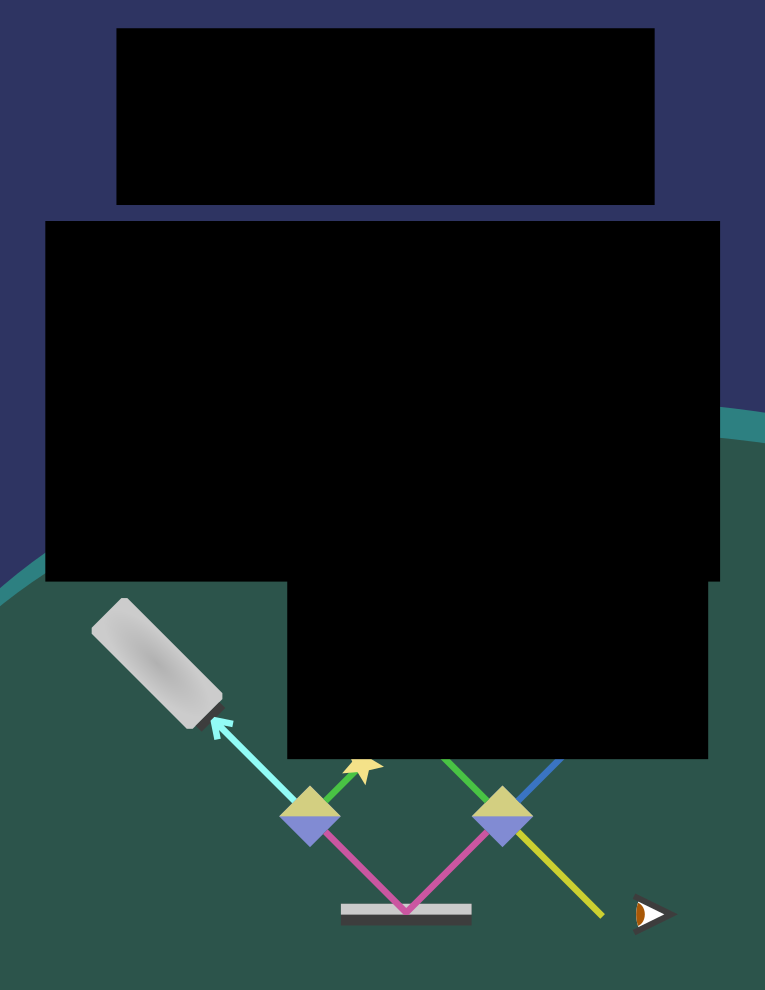
\includepdf[pages=-, offset=72 -36]{img/cover.pdf}

%%%%%%%%%%%%%%%%%%%%%%%%
% EDITION TIPS
%%%%%%%%%%%%%%%%%%%%%%%%

\cleardoublepage

This document was generated with the 2015 distribution of \LaTeX.

\vfill

\includegraphics[height=20pt]{img/0-CreativeCommons-by-sa.png}

2012-2015 Iagoba Apellaniz. This work is licensed under the Creative Commons
Attribution-ShareAlike 4.0 International License. To view a copy of this
license, visit
\href{http://creativecommons.org/licenses/by-sa/4.0/deed.en_US}
{http://creativecommons.org/ licenses/by-sa/4.0/deed.en\_US}.
\clearpage

%%%%%%%%%%%%%%%%%%%%%%%%
% PROLOGE
%%%%%%%%%%%%%%%%%%%%%%%%

\section*{Prologue}
\setcounter{page}{1}
\pagenumbering{roman}
\fancyfoot[LE,RO]{\thepage}

This work is part of doctoral project which I started on the sumer of 2013.
This work collects part of the research I have done on those previous fruitful years.
I will try to be as clear as possible throughout all the thesis
This way I hope it will be readable by any person with a bachelor in science, particularly in physics.
With that in mind the first and the second chapter will be used to introduce the reader into the context on which this thesis was written as well as the basic notions of Quantum Metrology, the enveloping field of the present work.
Even though I write this thesis for a broad audience in mind, a basic notion on quantum physics and statistics is needed to follow it properly.
For instance, I will assume among other things that the reader knows what probability is and which are its properties or what a quantum state is and what it represents.
I will give references where to find such complementary material when necessary.

This research I publish in a thesis form is part of the work done within the Research Group in Quantum Information in which Prof. G\'eza T\'oth is the group leader and principal investigator.
I have to mentions the rest of the members of the group Dr. Philipp Hyllus, Dr. Giuseppe Vitagliano, Dr. I\~nigo Urizar-Lanz, Dr. Z\'oltan Z\'inboras and Dr. Matthias Kleinmann at the time I was working on the projects of this thesis. Some of them may still be part of the group and some not.
Apart from the group of G\'eza T\'oth based in Bilbao, Spain, this thesis also collects some work done in collaboration with the Theoretical Quantum Optics (TQO) group lead by Prof. Otfried G\"uhne at the University of Siegen, Germany, and the group of Prof. Carsten Klempt at the Leibniz University in Hannover, based also in Germany. The last one is an experimental group specialized on the creation of exotic quantum states for a very many particle number with a variety of applications in quantum technology.

\begin{flushright}
  Iagoba Apellaniz

  30 of September of 2016, Bilbao
\end{flushright}


\section*{Publications}
{\setlength{\parindent}{0cm}
G\'eza T\'oth and Iagoba Apellaniz.
\textit{Quantum metrology from a quantum information science prespective.}
Journal of Physics A: Mathematical and Theoretical, \textbf{47} 424006, 2014.
\vspace{6pt}

Iagoba Apellaniz, Bernd L\"ucke, Jan Peise, Carsten Klempt and G\'eza T\'oth.
\textit{Detecting metrologically useful entanglement in the vicinity of Dicke states.}
New Journal of Physics, \textbf{17} 083027, 2015.
\vspace{6pt}

{\large\bf Preprints}

Iagoba Apellaniz, Matthias Kleinmann, Otfried G\"uhne and G\'eza T\'oth.
\textit{Optimal detection of metrologically useful entanglement.}
arXiv:1511.05203.
\vspace{6pt}

{\large\bf Out of the scope of this thesis}

Giuseppe Vitagliano, Iagoba Apellaniz, I\~nigo Luis Egusquiza and G\'eza T\'oth.
\textit{Spin squeezing and entanglement for arbitrary spin.}
Physical Review A, \textbf{89} 032307, 2014.
\vspace{6pt}

Giuseppe Vitagliano, Iagoba Apellaniz, Matthias Kleinmann, Bernd L\"ucke, Carsten Klempt and G\'eza T\'oth.
\textit{Entanglement and extreme spin squeezing of unpolarized states} arXiv:1605.07202.
}

%%%%%%%%%%%%%%%%%%%%%%%%
% TABLE OF CONTENTS
%%%%%%%%%%%%%%%%%%%%%%%%

\vspace*{100pt}
\tableofcontents

%%%%%%%%%%%%%%%%%%%%%%%%
% FIGURES TABLES, ETC
%%%%%%%%%%%%%%%%%%%%%%%%
\section*{Abbreviations, figures and tables}
\fancyfoot[LE,RO]{\thepage}
\subsection*{Abbreviations}
\hspace{7pt}
\begin{tabular}{l c l}
  BEC & - & Bose-Einstein condensate \\
  CLT & - & Central limit theorem \\
  HL  & - & Heisenberg limit \\
  HS  & - & Heisenberg scaling \\
  PDF & - & Pobability distribution function \\
  QFI & - & Quantum Fisher information \\
  SNS & - & Shot-noise scaling \\
  SNL & - & Shot-noise limit \\
  SLD & - & Symmetric logarithmic derivative \\
  SQL & - & Standard quantum limit \\
\end{tabular}

\makeatletter
\newcommand\listoffigurename{Figures}
\newcommand\listoftablename{Tables}
\renewcommand\listoffigures{
  \subsection*{\listoffigurename}
  \@starttoc{lof}
}
\renewcommand\listoftables{
  \subsection*{\listoftablename}
  \@starttoc{lot}
}
\makeatother
\listoffigures
\listoftables

%%%%%%%%%%%%%%%%%%%%%%%%
% THESIS
%%%%%%%%%%%%%%%%%%%%%%%%

\cleardoublepage

\pagenumbering{arabic}
\fancyfoot{}
%!TEX root = main.tex

\thiswatermark{\centering
\put(0,-110){\includegraphics[height=2.5cm]{img/0-Ztf.png}}
\put(430,-100){\includegraphics[height=2cm]{img/0-Ehu.png}}
}

\begin{center}

\vspace*{20pt}
\textsc{\LARGE University of the Basque Country}

\vspace{20pt}
\textsc{\Large PhD Thesis}

\vspace{50pt}
\hrule

\vspace{16pt}
{\huge \bfseries Lower bounds on quantum metrological precision}
\vspace{16pt}

\hrule
\vspace{40pt}

\begin{minipage}{0.4\textwidth}
\begin{flushleft} \large
\emph{Author:}


M. Sc. Iagoba \textsc{Apellaniz}
\end{flushleft}
\end{minipage}
\begin{minipage}{0.4\textwidth}
\begin{flushright} \large
\emph{Director:}

Prof. G\'eza \textsc{T\'oth} %TODO: Check Geza's name
\end{flushright}
\end{minipage}

\vspace{40pt}
\includegraphics[width=0.8\hsize]{img/0-cover3Dpicture.png}
\vfill

% Bottom of the page
{\large \today}

\end{center}

\cleardoublepage

\cleardoublepage
\setcounter{page}{1}

%%%%%%%%%%%%%%%%%%%%%%%%
% DEDICATION PAGE
%%%%%%%%%%%%%%%%%%%%%%%%
\vspace*{100pt}
\begin{center}
\emph{To my parents, my family}

\emph{and to all the people}

\emph{I have had around those years.}
\end{center}

\cleardoublepage

\fancyfoot[LE,RO]{\thepage}
\addcontentsline{toc}{section}{Acknowledgments}
\section*{Acknowledgments}

\lettrine[lines=2, findent=3pt,nindent=0pt]{I}{}want to thank the people that has supported me in this endeavor.
Especially, I want to acknowledge my office and discussion mates, Giuseppe Vitagliano and I\~nigo Urizar-Lanz as well as Phillip Hyllus, Matthias Kleinmann and Zolt\'an Zimbor\'as.
A special thank to my director G\'eza T\'oth for all the offered support, without whom my work at hand would not be possible.
I also want to thank more people from the department I belong to at the University of the Basque Country, the Department of Theoretical Physics and the History of Science.
I appreciate the effort done by people like I\~nigo L. Egusquiza in promoting the Ph.D. program of the Department of Theoretical Physics, which has successfully promote plenty of researchers now immersed in wonderful and leading edge research projects world wide.
Also I want to acknowledge the Ph.D. students from different departments for the friendship atmosphere one can enjoy working there at this \emph{our} university.

I have been visiting several research groups during those years and I don't forget them, they have accept me as one more between them.
So I want to thank a very especial research group for me, the Theoretical Quantum Optics group at the University of Siegen.
I would really like to mention the names of all of them but I think it would be quite heavy for the average reader of this thesis.
Thank you guys!
Also I want to thank people from the group QSTAR at Florence, Italy.

On the other hand I also felt very comfortable at my university, the University of the Basque Country, but I want to thank especially the people that make me grow in all ways as person.

\cleardoublepage

%%%%%%%%%%%%%%%%%%%%%%%%
% HEADINGS AND PAGE NUM.
%%%%%%%%%%%%%%%%%%%%%%%%

\renewcommand{\headrulewidth}{0.5pt}
\fancyfoot[LE,RO]{\thepage}
\fancyhead[LE]{\rightmark}
\fancyhead[RO]{\leftmark}

%%%%%%%%%%%%%%%%%%%%%%%%
% REDEFINE TITLE FORMAT
%%%%%%%%%%%%%%%%%%%%%%%%
\titleformat{\section}[display]
{\vspace*{150pt}
\bf\Huge}
{\hspace{-72pt}{\textcolor{grey}{\thesection}} \hspace{38pt} {\textcolor{white}{#1}}}
{0pt}
{}
[]
\titlespacing*{\section}{108pt}{10pt}{60pt}[20pt]


% Section: Introduction
\lettrine[lines=2, findent=3pt,nindent=0pt]{I}{n} the recent years...

The figure of merit for the precision is the inverse of the variance normalized with the number of particles, $(\Delta \Theta)^{-2}/N$. It has the following properties:

(i) The bigger it is the bigger is the precision

(ii) It is normalized so for the best separable state it is 1.
For greater values than 1 it would be a non-classical sign.

SQL

\be
  (\Delta \Theta)^{-2} \le N
\ee

HL

\be
  (\Delta \Theta)^{-2} \le N^2
\ee

This thesis consists of 4 well differentiated parts, apart from the current introduction, on which different topics are developed.
In the first part, we will introduce the reader onto the research field of quantum metrology.

Brief comments on the notation: $\text{c}_{\Theta}$ and ${\rm s}_{\Theta}$ stand for $\cos\Theta$ and $\sin\Theta$ respectively, probably some other trigonometry function is shortened.
We will omit the use of the tensor-product notation, $\otimes$, if there is not necessary for the correct comprehension of the text

\section[Backgroud in quantum metrology]
{Background in quantum metrology}
\thiswatermark{\put(1,-241){\color{l-grey}\rule{84pt}{48pt}}
\put(84,-241){\color{grey}\rule{410pt}{48pt}}}


\quotes{Roger J. Barlow}{In the real world, doing real experiments, statistics began to matter}

\vspace{0pt}
\lettrine[lines=2, findent=3pt,nindent=0pt]{I}{n} this chapter, we will study the basics of quantum metrology, which stands for the study of metrology enhanced by quantum phenomena.
First of all, metrology, as the science of measuring, has played an essential role in the development of science and technology.
Metrology studies several aspects of the estimation process, for example, which strategy to follow in order to improve the precision of the estimation.
Metrology also covers all intermediate processes, from the design aspects of a precise measuring device, to the most basic mathematical concepts that arise from the formulation of the different problems, which lead at the end to a more complete picture of what metrology is.

Historically, with the discovery of quantum theory and the subsequent development of quantum mechanics, new opportunities emerged for advances in metrology in the early decades of the twentieth century.
Later in the last decades of the twentieth century, together with the arrival of concepts like \emph{qubit} and \emph{quantum cryptography}, quantum theory embraced the so-called quantum information theory, which merges the notions of theory of information and computer science with quantum mechanics.
Pushed by the developments of quantum technologies, quantum information attracted much attention from the scientific community.
Moreover, those emerging fields rapidly became into very interesting interdisciplinary playgrounds of science with many scientists as well as resources involved.

At this point, we want to mention that the role of entanglement, an exclusive feature of quantum mechanics which cannot be described using classical probabilistic theories, is essential in this context.
Said this, entanglement is also at the center of the theory of quantum metrology.
Throughout the thesis we will focus mainly on the achievable precision for different systems and schemes.

On the other hand, another very important field of science must be mentioned.
We are talking about statistics, without which many descriptions of the actual and past physical findings would lack of the rigorous interpretation needed.
It basically helps to analyze raw data to make it readable from the human perspective.

This chapter is organized as follows.
In Section~\ref{sec:bg-statistics-and-stimation}, we introduce the basic concepts of statistics and estimation theory, focusing on what is necessary for the understanding of this thesis.
In Section~\ref{sec:bg-quantum-mechanics-for-metrology}, we present the necessary tools of quantum mechanics used throughout the text.
Finally in Section~\ref{sec:bg-quantum-metrology}, we arrive at the main set of tools used in the quantum metrology framework and by extension in the present work.

\subsection{Background in statistics and theory of estimation}
\label{sec:bg-statistics-and-stimation}

In this section, we will enumerate the basic concepts of statistics as well as the estimation process.
As we said, the main mathematical tools used by metrology belong to statistics.
Moreover, we are especially interested in estimation theory which shows how to properly estimate some quantity based on some data sample.
The data can be of any kind.
For instance, the data sample might be a set of the heights of a basketball team, or the outcomes of coin tosses, or even the wavelengths of photons coming out of some radioactive sample.
The aim of this section is to give the reader sufficient material to follow this thesis\footnote{
For a more detailed introduction to statistics, see Refs.~\cite{Riley2006, Barlow1989}}.

\subsubsection{Probability, data samples, average and variance}

The probability indicates the relative chance of an event to happen.
For instance, if there is a box with 10 red balls and 5 blue balls and assuming we extract on of them randomly, the probability of obtaining a blue ball is given by $\frac{n_{\text{blue}}}{n_{\text{total}}}=\frac{5}{10+5}=\frac{1}{3}$.
In the same way, the probability of obtaining a red ball is $\frac{n_{\text{blue}}}{n_{\text{total}}}=\frac{2}{3}$.
Note that some properties of the probabilities arise from simple example.
First, the probability of any event to happen is always given by a number in between zero and one.
Second, the sum of the probabilities of all possible events, in this case either blue or red, sum up to one.

With a data sample at hand, we face the task of analyzing the data to extract the relevant properties from it.
We assume that the data sample always comes from a population sample which represents all the available data before the measurements.
In general, the data sample might not be complete in the most general case (one could lose some data on the measuring process, or the population might be so large that we can only measure a small portion of it).
The measurement itself might induce some error in the data too (a measuring device always has an error when estimating a continuous magnitude, e.g., the height of people).
Hence, the data sample inherits a probability number for each of its data elements.
In the subsequent paragraphs, we will describe these relations between the data sample and the corresponding probabilities, and we will enumerate the most useful properties and formulas.

First of all, we will explain our notation which follows mainly the one used in Ref.~\cite{Riley2006}.
The outcome of magnitude we would like to measure from the data population is called a random variable.
First, when measuring some random variable $X$, a probability distribution function (PDF) gives the probability of $x$ to come out of the measurement and it is denoted by $\prob(X{=}x)$.
Second, due to the random nature of the measurement, the $N$ elements of a data sample are considered outputs of $N$ different random variables with their corresponding $N$ values as $\{X_i{=}x_i\}_{i=1}^N$, or $\bs{X}{=}\bs{x}$ for short.
The joint probability of those random variables is in general not separable.
This is due to the fact that the data sample elements could depend on the rest of outcomes or some other more complex relation that makes the most general case to be not separable from the probabilistic point of view.
Therefore we define the PDF of the data sample as an $N$-variable function
\be
  \prob(\bs{X}{=}\bs{x}) \equiv \prob(X_1{=}x_1,X_2{=}x_2,\dots,X_N{=}x_N).
\ee
In the case of separable probabilities, this is written as
\be
  \label{eq:bg-separable-likelyhood}
  \prob(\bs{X}{=}\bs{x}) = \prod_{i=1}^N\prob(X_i{=}x_i)
\ee
which is the case in many relevant situations.

When some indirect property of the system is defined as a function that depends on the measured random variables, the result is also a new random variable with another assigned PDF.
For example, we measure the position of a body at some moment.
If the system was at rest at the origin when $t=0$ and assuming that the acceleration is constant, then from the measured final position one could infer the value of the acceleration by using $A=2X/t^2$, where $X$ denotes the final position at instant $t$ and $A$ the acceleration.
If $X$ is a random variable, which is the general case when measuring the position of some physical system, then the probability assigned to $A$ is computed by
\be
  \prob(A{=}a) = \left.\frac{\text{d}X}{\text{d}A}\right|_{A=a}\prob(X{=}x)=\frac{2}{t^2}\prob(X{=}x).
\ee
In general, for multiple random variable, we require the following identity
\be
  |\prob(\bs{X}{=}\bs{x})\,\text{d}x_1\text{d}x_2\dots\text{d}x_N|=|\prob(\bs{Y}{=}\bs{y})\,\text{d}y_1\text{d}y_2\dots\text{d}y_N|,
\ee
which leads to some interesting formulas we will discuss later.

We now stick to the simplest case in which the data consists of a collection of values describing the same physical one-dimensional data population.
We assume that all the outcomes are independent between each other.
Hence, the PDF is of the form of Eq.~\eqref{eq:bg-separable-likelyhood}.
Some definitions, useful to mention in this thesis, arise for these kind of data samples: the average, variance, and the statistical moments and central moments.
The arithmetic average (there are other types of average one can find in the literature) is computed as
\be
  \overline{x}=\frac{1}{N}\sum_{i=1}^N x_i.
\ee
The variance, which is related to the spread of the data, is computed as
\be
  \sigma^2=\frac{1}{N}\sum_{i=1}^N (x_i-\overline{x})^2,
\ee
where $\sigma$ is the standard deviation.
Different statistical moments are computed by $\overline{x^r}=\frac{1}{N}\sum x_i^r$, while central moments, i.e., statistical moments that are invariant under a global translation of the parameter space, are of the form of $c_r=\frac{1}{N}\sum (x_i-\overline{x})^r$.
Note that the variance is the second central moment of the data samples.
For completeness, when each element of the data consists of more than a single magnitude the co-variance between two magnitudes is obtained as
\be
  V_{X,Y} = \frac{1}{N}\sum_{i=1}^N (x_i-\overline{x})(y_i-\overline{y}),
\ee
where it represents how both magnitudes influence each other.
As an example, we have the two magnitudes measured simultaneously $(v_i,a_i)$, where $v_i$ is the velocity and $a_i$ the acceleration of a body, in a experiment to estimate the friction coefficient of the air.

We will try to keep this distinction between data sample and data population as clear as possible.
The data population is represented in most cases by the probability distribution function.
In general, the mean values of any function $g(x)$ over the data sample are denoted with a bar over a lowercase variable, e.g., $\overline{x^r}$ for the $r$-th moment over the data sample or $\overline{g(x)}$ for the average of $g(x)$ itself.
On the other hand, the mean values of any function applied to the data population $g(X)$ is denoted following some textbooks by $\text{E}[g(X)]$, e.g., the $r$-th moment over the data population is $\text{E}[X^r]$.
One clearly may distinguish two cases when we talk about data populations.
While the data sample is always consist of discrete data elements, the data population can be represented by a PDF for discrete values or it can be represented by a PDF for values that can take any real number.
For completeness, here are expressed the two definitions for the mean value over the data population, i.e., represented by a PDF, of a function $g(\bs{X})$ by
\be
  \label{eq:bg-expectation-value-of-any}
  \text{E}[g(\bs{X})] = \lcor
  \begin{aligned}
    &\int g(\bs{x}) \prob(\bs{X}{=}\bs{x})\,\text{d}^N \bs{x},\\
    &\sum_{i,j,\dots} g(\bs{x}) \prob(\bs{X}{=}\bs{x}).
  \end{aligned}
  \right.
\ee
At this point, one more straight forward definition needs our attention, the variance of a function $g(X)$ over the data population is denoted by $\text{V}[g(X)] \equiv \text{E}[g(X)^2] - \text{E}[g(X)]^2$.

\subsubsection{Estimators and Fisher information}
\label{sec:bg-estimators}

Let us suppose that the data sample has encoded some desired parameters $\bs{a}\equiv(a_1,a_2,\dots)$.
The underlying probability, in general also unknown, may be conditioned by the real values of the parameters $\bs{a}$.
The probability of the data sample is therefore written as
\be
  \prob(\bs{X}{=}\bs{x}|\bs{a}),
\ee
where "$|\bs{a}$" indicates its dependency on these parameters.
At this point, note that an estimate of one of the desired parameters must be based on the data sample elements.
A function of this type is called the \emph{estimator} and it is connected with the PDF of the data population.
Hence as mentioned before, an estimator of $a$, one of the unknown parameters, is denoted by $\hat{a}$ and the PDF associated to it is computed from the PDF of the data population as
\be
  \prob(\hat{a}|\bs{a})\,\text{d}\hat{a} = \prob(\bs{x}|\bs{a})\,\text{d}x_1\text{d}x_2\dots\text{d}x_N.
\ee
For short, we have omitted writing "$\bs{X}{=}$", thus the conditional joint probability of $N$ random variables $\bs{X}$ is written simply as $\prob(\bs{x}|\bs{a})$.

As we said, an estimator is defined to be a function of the data sample.
For example, one of such estimators is the estimator of the mean value of the population, in general unknown.
The mean value of the data population, which in general we do not have access to, is denoted usually by $\mu$.
Note that $\mu$ is in general different from the mean value of the data sample $\overline{x}$.
A valid estimator for the mean value $\mu$ would be the mean itself of the data sample, i.e., $\hat{\mu}=\overline{x}$.

An important notion of an estimator is its \emph{efficiency}.
The smaller the variance of the estimator the more efficient it is.
Remember than an estimator is considered a random variable so it must have a variance when our knowledge about the population is incomplete, i.e., when we estimate it from the data sample.

Focusing into what it is more interesting for of this thesis, an estimator of any kind has a theoretical lower bound for its variance.
For the proof of the previous statement, which we will compute for continuous random variables without losing of generality, we start with the normalization formula of a given PDF
\be
  \int \prob(\bs{x}|\bs{a})\,\text{d}^N\bs{x} = 1.
\ee
Next, we compute the partial derivative over $a$, one of any of the unknown parameters, such that
\be
  \label{eq:bg-expectation-value-of-logarithm}
  \int \partial_a\prob(\bs{x}|\bs{a})\,\text{d}^N\bs{x} = \int \partial_a\big(\ln  \prob(\bs{x}|\bs{a})\big) \prob(\bs{x}|\bs{a}) \,\text{d}^N\bs{x} = 0,
\ee
where for the second equality we used the identity for logarithmic derivatives.
From Eq.~\eqref{eq:bg-expectation-value-of-any}, it turns out that the Eq.~\eqref{eq:bg-expectation-value-of-logarithm} is the expectation value of $\partial_a(\ln\prob)$.
Finally, if we have an \emph{unbiased} estimator, i.e., an estimator for which the expectation value $\text{E}[\hat{a}]$ coincides with true value $a$ of the unknown parameter, the partial differentiation of $\text{E}[\hat{a}]$ over $a$ must be equal to one.
Therefore, we apply similar identities as in Eq.~\eqref{eq:bg-expectation-value-of-logarithm} to arrive at
\be
  \label{eq:bg-expectation-of-estimator-derivated}
  \begin{split}
    \partial_a\text{E}[\hat{a}] &= \partial_a a
    = \partial_a \int \hat{a} \prob(\bs{x}|\bs{a})\,\text{d}^N\bs{x} \\
    &=  \int \hat{a} \partial_a\prob(\bs{x}|\bs{a})\,\text{d}^N\bs{x} =  \int \hat{a} \partial_a\big(\ln  \prob(\bs{x}|\bs{a})\big) \prob(\bs{x}|\bs{a}) \,\text{d}^N\bs{x} = 1,
  \end{split}
\ee
where we have used the definition of the expectation value for continuous variables Eq.~\eqref{eq:bg-expectation-value-of-any} and we use the fact that the estimator is not a function of the parameter $a$.

At this point, we invoke the Schwartz inequality for two real multidimensional functions $g(\bs{x})$ and $h(\bs{x})$ such that $(\int g h \,\text{d}^N\bs{x})^2\leqslant (\int g^2 \,\text{d}^N\bs{x}) (\int h^2 \,\text{d}^N\bs{x})$.
With this, we can follow step by step the following recipe to obtain a lower bound for the variance of a general estimator.
First the definition of the variance over the data population looks like
\be
  V[\hat{a}] = E[(\hat{a}-a)^2] = \int (\hat{a} - a)^2\prob(\bs{x}|\bs{a})\,\text{d}^N\bs{x},
\ee
remember that the estimator is assumed to be unbiased.
Second, subtracting $a$ times Eq.~\eqref{eq:bg-expectation-value-of-logarithm} to Eq.~\eqref{eq:bg-expectation-of-estimator-derivated} the following holds,
\be
  \int (\hat{a}-a)\partial_a\big(\ln  \prob(\bs{x}|\bs{a})\big) \prob(\bs{x}|\bs{a})\,\text{d}^N\bs{x} = 1
\ee
because $a$ is not a function of $\bs{x}$.
Hence, using the Schwartz inequality we can write
\be
  \label{eq:bg-classical-cr-bound-and-fi}
  \text{V}[\hat{a}] = \int (\hat{a} - a)^2\prob(\bs{x}|\bs{a})\,\text{d}^N\bs{x} \geqslant \frac{1}{\int \lcua\partial_a\big(\ln \prob (\bs{x}|\bs{a}) \big)\rcua^2 \prob (\bs{x}|\bs{a})\,\text{d}^N\bs{x}},
\ee
which is also known as the Cram\'er-Rao bound or the Fisher inequality.
The denominator in the right hand-side is called generally the Fisher information or simply information.

With this review of the most interesting properties of "classical" metrology, from the point of view of this thesis, we conclude this section.
In the next section, we will discuss some properties of the quantum mechanics and then we will follow with another section which presents the basis of quantum metrology.

\subsection{Quantum mechanics from metrology perspective}
\label{sec:bg-quantum-mechanics-for-metrology}

The ubiquitous probabilistic nature of quantum mechanics makes us to work with probabilities on a regular basis.
Moreover, if one studies fields connected to experiments or some short of physical realizations, this probabilistic nature of quantum mechanics becomes even more visible.
On the other hand, exotic features such as entanglement arise from quantum mechanics, which is directly connected with the probabilistic notions explained before.
The present section is intended to describe quantum systems from the point of view of metrology.

\subsubsection{The quantum state, multiparticle state and entanglement}
\label{sec:bg-the-quantu-state}

A formal mathematical description of the quantum state is given next.
This also allows us to introduce some notation used throughout the thesis.
A \emph{state} in quantum mechanics lives in a Hilbert space, $\mathcal{H}$.
The state, $\rho$, has the following properties:
\begin{enumerate}
  \item
  It is Hermitian, so it is invariant under the complex transposition, $\rho=\rho^\dagger$ and all its eigenvalues are real.
  \item Its trace is equal to one, $\tr(\rho)=1$.
  \item It is positive semi-definite, i.e, all its eigenvalues are bigger or equal to zero, $\rho=\sum_{\lambda}p_\lambda \Pi_\lambda$ where $p_\lambda\geqslant 0$ and $\Pi_\lambda\equiv\ketbra{\lambda}{\lambda}$ is the projector of the eigenstate $\ket{\lambda}$, a vector state satisfying the following eigenvalue equation $\rho\ket{\lambda}=p_{lambda}\ket{\lambda}$.
  From (ii), it follows that $\sum_\lambda p_\lambda = 1$.
  \item If all $p_\lambda$ are zero except one, the state is called a pure state and is equivalent to the projector of such eigenstate $\rho=\Pi_\lambda=\ketbra{\lambda}{\lambda}$.
  \item Using the properties (iii) and (iV), it follows that the quantum states form a convex set where the extreme must be pure states.
  \item An expectation value of an observable $\mathcal{O}$ is computed as $\expect{\mathcal{O}}=\tr(\mathcal{O}\rho)$.
  To make a connection with the previous section, the state represents the so-called data population, hence using the notation in Sec.~\ref{sec:bg-statistics-and-stimation},  $\expect{\mathcal{O}}\equiv\text{E}[\mathcal{O}]$.
\end{enumerate}

The composite system of $N$ different parties live in the Hilbert space $\mathcal{H} = \mathcal{H}^{(1)}\otimes\mathcal{H}^{(2)}\otimes\cdots\otimes\mathcal{H}^{(N)}$ or $\mathcal{H} = \bigotimes_{i=1}^N\mathcal{H}^{(i)}$ for short, where $\otimes$ stands for tensor product.
For instance, this composite Hilbert space could be used to represent a many-particle system, in this case $N$ particles.
A \emph{separable} state in this Hilbert space can be written as
\be
  \label{eq:bg-separable-state-definition}
  \rho_{\text{sep}} = \sum_{i}p_i\rho_i^{(1)}\otimes\rho_i^{(2)}\otimes\cdots\otimes\rho_i^{(N)},
\ee
where $p_i$ are convex weights that add up to one and are equal to or bigger than zero.
If a state cannot be written like Eq.~\eqref{eq:bg-separable-state-definition}, the state is said to be \emph{entangled}.
We mention it as a formal description of the entanglement \cite{Guehne2009, Luis2004}.
One may note at this moment, that relaxing the requirements of Eq.~\eqref{eq:bg-separable-state-definition}, one can lead to different classifications of the states.
Concepts like genuine multipartite entanglement, $k$-producible states, or entanglement depth, among others, arose from weaker constraints than Eq.~\eqref{eq:bg-separable-state-definition} \cite{Guehne2009, Luis2004}.

It is important to describe one of such classifications in order to characterize the different levels or multipartite entanglement followed in this work.
We call a state $k$-producible, if it \emph{can} be written as a mixture of the tensor product of different multipartite states with at most $k$ parties in each,
\be
  \label{eq:bg-k-producible-estate}
  \rho_{k\text{-pro}} = \sum_i p_i\rho^{(\alpha,\dots,\beta)}_i \otimes \rho^{(\gamma,\dots,\delta)}_i\otimes \dots,
\ee
where superscript indexes between parenthesis go from 1 to $N$ and denote to which parties belong to the state, and where each index appears once in each sum element.
For instance a separable state like Eq.~\eqref{eq:bg-separable-state-definition} is 1-producible as well as $N$-producible.
If a state cannot be written as $k$-producible, then it must be $(k+1)$-entangled.
This defines the entanglement depth, see Figure~\ref{fig:bg-separability-k-producibility-circle}.
Later on, these concepts of entanglement and entanglement depth will arise naturally on the metrological framework \cite{Toth2014}.
\begin{figure}[htp]
  \centering
  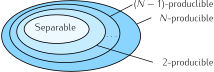
\includegraphics[scale=1.2]{img/BG_separability_k_producibility_circle.pdf}
  \caption[Diagram for $k$-producibility sets]{
  $k$-producible set of states contains $k-1$-producible states. Based on the Eq.~\eqref{eq:bg-k-producible-estate}, one can argue that a state that cannot be written as $k$-producible must be $k+1$-entangled or equivalently has $k+1$ entanglement depth. A separable state can always be written as 1-producible which on the other hand is its original definition.}
  \label{fig:bg-separability-k-producibility-circle}
\end{figure}

\subsubsection{Angular momentum operators on multiparticle systems}
\label{sec:bg-angular-momentum-operators}

Besides those concepts, we present a set of operators that will appear many times in all chapters, namely the angular momentum operators.
Again these definitions allow us to introduce much of the notation used on this book.
For a single party with discrete $d$ levels, and therefore with a spin $j=(d-1)/2$, the eigenvalue equation for the angular momentum projection operators are
\be
  j_l^{(n)}\ket{m}_l^{(n)} = m \ket{m}_l^{(n)}
\ee
for $m=-j,\dots,+j$, where $l=x,y,z$.
It is usual to omit the subscript of $\ket{m}_l^{(n)}$ when $l=z$ because it is the preferred direction for many authors and the superscript ($n$) can also be omitted when the single-particle states are given in an ordered form to build a multiparticle state, i.e., $\ket{\psi} = \ket{m_1}\ket{m_2}\dots\ket{m_n}$ where we also omitted writing the tensor product operator $\otimes$ in between single-particle states.
In many cases, it is also usual to merge all into a single ket state $\ket{\psi}=\ket{m_1 m_2 \dots m_N}$ for simplicity\footnote{
This notation is normally used in many-body quantum mechanics, see Refs.~\cite{Cohen-Tannoudji1977, Sakurai2010}.}.

The square of the total angular momentum, $\bs{j}^2=j_x^2+j_y^2+j_z^2$, for a single party $(n)$ acts on any state simply as
\be
  (\bs{j}^2)^{(n)}\rho=j_n(j_n+1)\rho,
\ee
where state must be defined in a Hilbert space containing $\mathcal{H}^{(n)}$, the Hilbert space of $n^{\text{th}}$ particle and where $j_n$ is the spin number of such a particle.
Note that in order to distinguish the spin number $j_n$ and the operators $j_l^{(n)}$ we may use the fact that the operators are attached to a Hilbert space with a superscript or even we can use a "hatted" notation to denote which of them is an operator like $\hat{j_l}$ and which is not.

The collective angular momentum projection operators $J_l$ are defined as the sum of their respective single-party spin operators $j_l^{(n)}$ such that they are extended to the remaining of the Hilbert spaces by tensor products of the identity operators defined for the rest of subspaces,
\be
  \label{eq:bg-total-angular-momentum-progection-operators}
  J_l = \sum_{i=1}^N \mtxid^{(1,\dots, i-1)} \otimes j_l^{(i)} \otimes \mtxid^{(i+1,\dots,N)} \equiv \sum_{i=1}^N j_l^{(i)},
\ee
where $\mtxid$ stand for the identity operator and the last formula is the most used since it is easy to note that the single-party operator must be extended in order to sum the correctly.
On the other hand, note that the squares of the different projections of total angular momentum are not equal to the sum of the square angular momentum projections of each of the parties.
Thus we obtain that
\be
  J_l^2 = \sum_{i,j}^N j_l^{(i)} j_l^{(j)} = \sum_{i=1}^N (j_l^2)^{(i)}+\sum_{i\neq j}^N j_l^{(i)} j_l^{(j)}.
\ee
Therefore, neither square of the total angular momentum is the sum of the square of all single-party angular momenta but
\be
  \bs{J}^2 = \sum_{i}^N \bs{j}^{(i)} + \sum_{l=x,y,z}\sum_{i\neq j}^N j_l^{(i)} j_l^{(j)},
\ee
where we separated the sum into two parts, the first one corresponds to the sum of all single party angular momentum projections squared and the second corresponds to the product of angular momentum projection operators of two distinct subsystems summed for all $l=x,y,z$.
Many more combinations of these single-party operators may arise in different contexts.
In the Appendix~\ref{app:angular-subspaces}, we discuss in more detail the different structures that arise from adding the angular momentum operators, e.g., the symmetric subspace or the singlet subspace.

\subsubsection{Dynamics of quantum systems}

The most basic evolution of the state is represented by unitary evolution operators denoted by $U$ and those are the only ones appearing throughout the thesis.
On the other hand, there are other types of dynamics involving particle loss, entropy changes in the system and open quantum systems in general.
These transformations are governed by master-equations such as the Lindblad equation \cite{Lindblad1976, Nielsen2000, Breuer2002}.

For the understanding of this thesis it is enough to present the unitary evolution operators.
We also restrict ourselves to the case in which the evolution is constant in time, so are in general the Hamiltonians of the metrological setups.
The unitary evolution operators is defined as
\be
  U = \exp(-i \alpha G)=\sum_{n=0}^{\infty} \frac{(-i \alpha G)^n}{n!},
\ee
where we use the matrix exponentiation in the last equality, $G$ represents a Hermitian operator usually called generator and $\alpha$ is the amount of change.
When a constant Hamiltonian $H$ acts on an initial state $\rho$, the state evolves in time as
\be
  \rho(t) = U\rho U^{\dagger} = e^{-i\frac{tH}{\hbar}} \rho e^{+i\frac{tH}{\hbar}}.
\ee
Note that all information we can extract from the system comes in the form of expectation values of different operators at different times, $\expect{\mathcal{O}}(t) = \tr(\mathcal{O}\rho(t))$.
When the state evolves in time but the operators are constant the picture of the system is called the Schrodinger-picture.
Using the cyclic property of the trace, $\tr(ABC) = \tr(CBA)$, the Heisenberg-picture, a dual interpretation of the same physical system in which the state remains the same while the operators evolve in time, emerges.
It is well known that the operators in this picture evolve as $\mathcal{O}(t) = U^{\dagger} \mathcal{O} U$, where $\mathcal{O}$ is the initial operator.
One can check different textbooks of quantum mechanics, just to mention some see Refs.~\cite{Cohen-Tannoudji1977, Sakurai2010}.

\subsection{Quantum metrology}
\label{sec:bg-quantum-metrology}

We summarize important recent advances in quantum metrology.
Simple metrological setups allow for encoding some desired parameter into the state of the system, thus from the readout of the final state one could infer it.
The basic ideas of quantum metrology emerge when one applies the notions of estimation theory to the intrinsic probabilistic nature of quantum mechanics.
Merging the probabilistic features of quantum mechanics and the estimation theory is not trivial.
Nevertheless, with the initial pioneering works of C. W. Helstrom, W. K. Wootters, and S. L. Braunstein and C. M. Caves, in 1969, 1981 and 1992-1994 respectively \cite{Helstrom1969, Wootters1981, Braunstein1992, Braunstein1994}, until the works of V. Giovannetti {\it et al}, and M. G. Paris, roughly two decades later \cite{Giovannetti2004, Paris2009}, the foundations of quantum metrology were stabilized.
% TD: important citations needed here!!
Later, advanced works in quantum metrology appeared \cite{Hyllus2010, Hyllus2012, Hyllus2010a, Kolodynski2010, Kolodynski2013}
together with experimental realizations \cite{Behbood2013, Koschorreck2011, Luecke2011} which raised the interest in this topic.
In this section, we will highlight the most important aspects of this field and with this we will conclude this chapter for presenting the background theory in which stands the work developed by the authors.

The most basic scheme for a metrological setup in the present context is the following.
First, a state $\rho$ is prepared followed by a general evolution represented by a mapping $\Lambda_{\theta}$ in which the unknown parameter $\theta$ is imprinted into the state.
Finally, the outgoing state is characterized by some measured quantity $\expect{M}$, which allows to infer the value of the parameter $\theta$.
Figure~\ref{fig:bg-preparation-encoding-estimation} illustrates the main steps of quantum metrology.
\begin{figure}[htp]
  \centering
  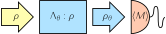
\includegraphics[scale=1.2]{img/BG_preparation_encoding_estimation.pdf}
  \caption[The estimation process in quantum metrology]{
  Sequence of the different steps for the basics of the estimation process in quantum metrology. First, an input state $\rho$ enters the region in which the unknown parameter $\theta$ is imprinted in it, for the most general case, represented with $\Lambda_{\theta}$. The state with the encoded parameter $\theta$ is measured and $\theta$ must be inferred from the measured quantity $\expect{M}$.}
  \label{fig:bg-preparation-encoding-estimation}
\end{figure}

In the many-particle case, most of the metrology experiments have been done in systems with simple Hamiltonians that do not contain interaction terms.
Such Hamiltonians cannot create entanglement between the particles.
A typical situation is that we rotate our many particle state by some angle and we want to estimate the rotation angle $\theta$.
It has been shown that particles exhibiting quantum correlations, or more precisely, quantum entanglement \cite{Guehne2009, Luis2004}, provide a higher precision than an ensemble with non-entangled particles.
The most important question is how the achievable precision of the angle estimation $\varian{\theta}$ scales with the number of particles.
Very general derivations lead to, at best,
\be
  \label{eq:bg-shot-noise-scaling}
  \varian{\theta}\sim \frac{1}{N}
\ee
for non-entangled particles.
The equation above is called \emph{shot-noise} or standard scaling, the term originating from the shot-noise in electronic circuits, which is due to the discrete nature of the electric charge.
On the other hand, quantum entanglement makes it possible to reach
\be
  \label{eq:bg-heisenberg-scaling}
  \varian{\theta}\sim \frac{1}{N^2}
\ee
which is called the \emph{Heisenberg} scaling.
Note that if the Hamiltonian of the dynamics has interaction terms, then these bounds can be surpassed \cite{Luis2004, Napolitano2011, Boixo2007, Braun2011, Roy2008, Choi2008, Rey2007}.

It is time to mention that the above calculations have been carried out for an ideal situation.
When an uncorrelated noise is present in the system, it turns out that for large enough particle number the scaling becomes shot-noise scaling. \cite{Demkowicz-Dobrzanski2012}.
The possible survival of a better scaling under correlated noise, under particular circumstances, or depending on some interpretation of the metrological task, is at the center of attention currently.
All these are strongly connected to the question of whether strong multipartite entanglement can survive in a noisy environment.

Finally, note that often, instead of $\varian{\theta}$ one calculates its inverse, which is large for high precision.
It scales as $\varinv{\theta}\sim N$ for shot-noise scaling and as $\varinv{\theta}\sim N^2$ for the Heisenberg scaling.

\subsubsection{Quantum magnetometry}
\label{sec:bg-quantum-magnetometry}

Without loss of generality, we present in this section the characterization of the precision of one of the simplest metrological tasks, namely the estimation of a homogeneous magnetic field based on the interaction between the system and the field.
In this section, we will mostly study the interaction of a system with a homogeneous field in the $z$-direction.
In the Chapter~\ref{sec:gm}, we will show a different situation in which the magnetic field changes linearly with the position of the system.
With the aim of estimating the strength of the magnetic field, a state is used in order to interact with it, coupling the magnetic moment of the state and the external magnetic field.
Finally, measuring how the state has changed one could in principle infer on the strength of the magnetic field.

In general, we will say that the magnetic moments of the states come exclusively from the spin angular momentum, neglecting any possible contribution from the orbital angular momentum.
This way the physics is simpler.
This is justified in the sense that most of the recent experiments in this context have been carried out with ion-traps, Bose-Einstein condensates (BEC) or at most cold atomic ensembles, which have indeed a negligible orbital angular momentum.

Beside this considerations, the interaction Hamiltonian can be written as
\be
  H = - \bs{\mu} \cdot \bs{B}
\ee
up to some constant factor.
Now in the simplest case we will choose the magnetic field to be pointing to some fixed direction, for instance, the $z$-direction.
So the magnetic field vector can be written as ${B}=B\bs{k}$, where $\bs{k}$ is the unitary vector pointing to the $z$-direction.
This way the estimation problem is much simpler, since one does not need to determine the direction of the magnetic field.

The magnetic moment of the system is proportional to the spin angular momentum, $\bs{\mu}=-\mu_\text{B} g_{\text{s}}\hbar^{-1} \bs{J}$, where $\mu_{\text{B}}$ and $g_{\text{s}}$ are the Bohr magneton and anomalous gyromagnetic factor respectively.
Finally, one can rewrite the interaction Hamiltonian as
\be
  \label{eq:bg-hamiltonian-homogeneous-field}
  H = \gamma B J_z,
\ee
where $\gamma = \mu_\text{B} g_{\text{s}}\hbar^{-1}$ and we have used the fact that $\bs{J}\cdot\bs{k}=J_z$.
Finally, the unitary operator leading the evolution of the system can be written as
\be
  \label{eq:bg-unitary-homogeneous-field}
  U = \exp(-i\theta J_z),
\ee
where the magnetic field strength is encoded into the phase-shift $\theta=-\mu_\text{B} g_\text{s} t B/\hbar$.
Here $\mu_\text{B}$ stands for the Bohr magneton and $g_\text{s}$ for the giro-magnetic constant for the spin angular momentum, and $t$ is the evolution time.

We have to mention as well that for large particle ensembles, typically only collective quantities can be measured in order to characterize the state on different phases of the metrological sequence, see Figure~\ref{fig:bg-preparation-encoding-estimation}.
Such collective quantities are in this case the angular momentum components defined in Eq.~\eqref{eq:bg-total-angular-momentum-progection-operators} and their combinations.
More concretely, we can measure the expectation values of any direction
\be
  \label{eq:bg-total-angular-momentum-projector-arbitrary-direction}
  J_{\bs{n}}:=\sum_{l=x,y,z} n_l J_l,
\ee
where $\bs{n}=(n_x,n_y,n_z)$ is a unit vector describing the direction of the component.

\subsubsection[Metrology with almost polarized states]{Metrology with almost polarized states, including spin-squeezed states}
\label{sec:bg-metrology-with-almost-polarized}

Let us present one of the basic approaches to calculate the metrological precision of a quantum setup.
In order to estimate the phase-shift $\theta$ we measure the expectation value of a Hermitian operator, which we will denote by $M$ in the following.
If the evolution time is a constant then estimating $\theta$ is equivalent to estimating the magnetic field strength $B$ in Eq.~\eqref{eq:bg-hamiltonian-homogeneous-field}.
The precision of the estimation can be characterized with the error propagation formula (EPF) as
\be
  \label{eq:bg-error-propagation-formula}
  \varian{\theta} = \frac{\varian{M}}{|\partial_\theta\expect{M}|^2},
\ee
where $\expect{M}$ is the expectation value of the operator $M$, and we used the assumption that $\expect{M}$ is a random variable and that it has a PDF that can relate $\prob(\expect{M}|\theta)$ with a PDF as a function of the estimator $\prob(\hat{\theta}|\theta)$, see the Section~\ref{sec:bg-estimators}, and for a recent review discussing this approach in detail, see Ref.~\cite{Kolodynski2010}.
Thus, the precision of the estimate depends on how sensitive $\expect{M}$ is to the change of $\theta$, and also on how large the variance of $M$ is.
Based on the formula Eq.~\eqref{eq:bg-error-propagation-formula}, one can see that the larger the slope $|\partial_\theta \expect{M}|$, the higher the precision.
On the other hand, the larger the variance $\varian{M}$, the lower the precision.
Figure~\ref{fig:bg-expect-m-evo} helps to interpret the quantities appearing in Eq.~\eqref{eq:bg-error-propagation-formula}.
\begin{figure}[htp]
  \centering
  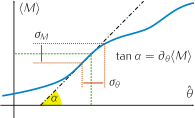
\includegraphics[scale=1.2]{img/BG_expect_m_evo.pdf}
  \caption[Error-propagation formula]{
  (Blue solid) Functional relation between the expectation value $\expect{M}$ and the estimator of the wanted parameter $\hat\theta$.
  (Green dashed) One to one correspondence when the estimator $\hat{\theta}$ is based on $\expect{M}$. (Red dotted) Obtaining the error of the estimate is based on Eq.~\eqref{eq:bg-error-propagation-formula}.
  The slope of the curve at that point, denoted with $\tan\alpha$, directly relates the uncertainty $\sigma_M$ on the measured quantity $\expect{M}$ and the error on the estimation $\sigma_\theta$.}
  \label{fig:bg-expect-m-evo}
\end{figure}

We focus on multi-partite systems of spin-$\frac{1}{2}$ particles, widely known in the field as qubits, for homogeneous magnetometry in order to simplify the discussion.
For this, let us start with an almost polarized state.
We present the state totally polarized along the $l$-direction as
\be
  \ket{+j}_l^{\otimes N}\equiv \ket{+j}_l^{(1)}\ket{+j}_l^{(2)}\cdots\ket{+j}_l^{(N)},
  \label{eq:bg-totally-polarized}
\ee
since it plays a very important role in quantum metrology when $l=y$. It is almost all the times one of the states that reaches the shot-noise scaling Eq.~\eqref{eq:bg-shot-noise-scaling} and saturates the shot-noise limit, which will appear later in this section.
In this case, the spin-vector of the ensemble, originally pointing into the $y$-direction, will be rotated.
The rotation after the evolution is used to estimate the strength of the magnetic field.
A way to measure the rotation suffered by the system is to measure the expectation value $\expect{J_x}$, which is zero at the beginning.

For small angles of $\theta$ and using the Eq.~\eqref{eq:bg-error-propagation-formula} after substituting $M$ by $J_x$, we arrive at
\be
  \label{eq:bg-error-propagation-measuring-jx}
  \varinv{\theta} = \frac{|\partial_\theta \expect{J_x}|^2}{\varian{J_x}},
\ee
for a state almost completely polarized along the $y$-axis.
Next, we have to compute these values for small angles of $\theta$.

To compute them we use the Heisenberg picture of the operator $J_x$, that after applying the unitary operator Eq.~\eqref{eq:bg-unitary-homogeneous-field}, is written as
\be
  J_x(\theta) = U^{i\theta J_z} J_x U^{-i\theta J_z} = \coss{\theta}J_x -  \sins{\theta} J_y,
\ee
where we also introduced a notation for trigonometric functions since they will appear many times in this work, $\coss{x} \rightarrow \cos(x)$, $ \sins{x}\rightarrow\sin(x)$ and $\tans{x}\rightarrow\tan(x)$.
Thus, the square of $J_x$ is simply
\be
  J_x^2(\theta) = \coss{\theta}^2J_x^2 -2 \coss{\theta}\sins{\theta}\{J_x,J_y\}+  \sins{\theta}^2 J_y^2,
\ee
where $\{A,B\}=AB+BA$ is the anti-commutator, since the operators may not commute in general and in this particular case it is not an exception.
Finally we compute the derivative with respect to $\theta$ of $\expect{J_x}$ as
\be
  \partial_{\theta}\expect{J_x}(\theta)=\partial_{\theta}\coss{\theta}\expect{J_x} - \partial_{\theta}\sins{\theta}\expect{J_y} = -\sins{\theta}\expect{J_x}-\coss{\theta}\expect{J_y},
\ee
where we used the linearity of the trace to compute the expectation value and the linearity of the derivative.

Hence, assuming that we are in the small angle limit to compute the Eq.~\eqref{eq:bg-error-propagation-measuring-jx}, we may take the terms proportional to $\sin(\theta)$ as zero.
Therefore, when we measure $\expect{J_x}$ to estimate the angle $\theta$, the precision of the estimation is given by
\be
  \label{eq:bg-error-propagation-measuring-jx-computed}
  \varinv{\theta} = \frac{|\coss{\theta}\expect{J_y}|^2}{\coss{\theta}^2\expect{J_x^2} - (\coss{\theta}\expect{J_x})^2} = \frac{\expect{J_y}^2}{\varian{J_x}}.
\ee

For the state totally polarized along the $y$-axis, the initial expectation values $\expect{J_x}$, $\expect{J_x^2}$ and $\expect{J_y}$ needed to compute the precision are
\be
  \begin{split}
    \expect{J_x}_{\text{tp}}  & = 0,\\
    \expect{J_x^2}_{\text{tp}}  & = \tfrac{N}{4},\\
    \expect{J_y}_{\text{tp}}  & = \tfrac{N}{2}.
  \end{split}
\ee
Thus, we obtain a precision that scales linearly with $N$,
\be
  \varinv{\theta}_{\text{tp}} = \frac{N^2/4}{N/4} = N.
\ee
Note that the totally polarized state Eq.~\eqref{eq:bg-totally-polarized} is a separable pure state with all particles pointing into the $y$-direction.
We obtained the shot-noise scaling, even with very simple, qualitative arguments

A way of improving the precision is considering that the variances of the angular momentum components are bounded by the Heisenberg uncertainty relation \cite{Kitagawa1993}
\be
  \varian{J_x}\varian{J_z} \geqslant \frac{1}{4}|\expect{J_y}|.
\ee
Due to decreasing $\varian{J_x}$, our state fulfills
\be
  \varian{J_x}<\frac{1}{2}|\expect{J_y}|,
\ee
where the main spin points along the $y$-axis and for totally polarized states $\varian{J_x}=\frac{1}{2}|\expect{J_y}|$ hold.
Such states are called \emph{spin-squeezed} states \cite{Kitagawa1993, Wineland1994, Sorensen2001, Ma2011} and they can in principal overcome the shot-noise scaling.

Next, we can ask, what the best possible phase estimation precision is for the metrological task considered in this section.
For that, we have to use the following inequality based on general principles of angular momentum theory
\be
  \label{eq:bg-total-angular-momentum-saturability}
  \expect{J_x^2+J_y^2+J_z^2} \leqslant \frac{N(N+2)}{4}.
\ee
Note that Eq.~\eqref{eq:bg-total-angular-momentum-saturability} is saturated only by symmetric multiparticle states, see Appendix~\ref{app:angular-subspaces}.
Together with the identity connecting the second moments, variances and expectation values
\be
  \varian{J_l} + \expect{J_l}^2 = \expect{J_l^2},
\ee
Eq.~\eqref{eq:bg-total-angular-momentum-saturability} leads to a bound on the uncertainty in the anti-squeezed direction, in this case $z$-direction, for the variance
\be
  \varian{J_z} \leqslant \frac{N(N+2)}{4} - \expect{J_y}^2 = \frac{N}{2} + \frac{N^2}{4}\lpar 1 - \frac{\expect{J_y}^2}{J_{\max}^2}\rpar,
\ee
where $J_{\max}$ is the maximum value a angular momentum component can take, i.e., $N/2$.
This leads to a bound in the precision when measuring $\expect{J_x}$ as
\be
  \label{eq:bg-unpolarize-states-are-better}
  \varinv{\theta} = \frac{\expect{J_y}^2}{\varian{J_x}}\leqslant 4\varian{J_z}\leqslant 2N + N^2\lpar 1 - \frac{\expect{J_y}^2}{j_{\max}}\rpar,
\ee
which indicates that the precision is limited for almost completely polarized states to the shot-noise scaling.
The bound above is not optimal, as for the fully polarized state we would expect $N$ and we obtain $2N$.

\subsubsection{The quantum Fisher information}
\label{sec:bg-qfi}

In this section, we review the theoretical background of the Fisher information, the Cram\'er-Rao bound and we introduce the quantum Fisher information.

First of all, we have already shown the Fisher information and the Cram\'er-Rao bound in the Section~\ref{sec:bg-estimators}.
The formula Eq.~\eqref{eq:bg-classical-cr-bound-and-fi} tells us that if we measure an operator, say $M$, and we know its probability distribution function $\prob(\expect{M}|\theta)$, we can bound the achievable precision.
In quantum mechanics the PDF of a state $\rho_\theta$ when measuring the operator $M$ is given by
\be
  \prob(m|\theta) = \tr({\Pi_{m}\rho_\theta}),
\ee
where $\Pi_{m}$ are the projector operators or the eigenstates on which $M$ is expanded, $M = \sum m \Pi_m$.
Following arguments found on Refs.~\cite{Giovannetti2004, Paris2009}, one can arrive at a universal bound valid for any kind of measurements.
This bound is called the quantum Cram\'er-Rao bound given as
\be
  \label{eq:bg-quantum-cr-bound}
  \varinv{\theta} \leqslant \qfif{\rho,J_z},
\ee
where $\qfif{\rho, J_Z}$ denotes the quantum Fisher information for the initial state $\rho$ and the unitary evolution generated by $J_z$.
In principle, it might be difficult to find the operator that leads to the best estimation precision just by trying several operators.
Fortunately, the Eq.~\eqref{eq:bg-quantum-cr-bound} gives us that upper bound that is valid for any choice on the measurement \cite{Helstrom1976, Holevo1982}.

As a direct consequence, based on Eq.~\eqref{eq:bg-error-propagation-formula} for any given $M$, we have that
\be
  \qfif{\rho,J_z} \geqslant \frac{|\partial_{\theta}\expect{M}|^2}{\varian{M}}
\ee
is an upper bound for concrete bounds based on the measurement scheme.
For example, when the rotation of the system is estimated by measuring $\expect{J_x}$ the quantum Fisher information is bounded from below by \cite{Pezze2009}
\be
  \label{eq:bg-pezze-bound}
  \qfif{\rho,J_z} \geqslant \frac{\expect{J_y}^2}{\varian{J_x}},
\ee
as it is directly infer from Eq.~\eqref{eq:bg-error-propagation-measuring-jx-computed}.

The quantum Fisher information can be computed by closed formulas such as
\begin{align}
  \label{eq:bg-qfi-definition-eigen-decomposition}
  \qfif{\rho,J_z} &= 2\sum_{\lambda,\nu} \frac{(p_\lambda-p_\nu)^2}{p_\lambda+p_\nu} |\braopket{\lambda}{J_z}{\nu}|^2, \\
  \label{eq:bg-qfi-definition-convex-roof}
  \qfif{\rho,J_z} &= \inf_{p_k,\psi_{k}} 4 \sum_{k}p_k \varian{J_z}_{\psi_k},
\end{align}
for the case of unitary evolution Eq.~\eqref{eq:bg-unitary-homogeneous-field} and where the state can be decomposed in its eigenbasis as $\rho=\sum_{\lambda}p_\lambda\ket{\lambda}$ in the first case, or where it is any arbitrary convex decomposition like $\rho=\sum_k p_k \ketbra{\psi_k}{\psi_k}$, used the later in the second case.
The first one is based on the eigen-decomposition of the state whereas the second is the convex-roof of $4\varian{J_z}$ \cite{Paris2009, Toth2013, Yu2013}.
Both formulas yield to the same expression for pure states
\be
  \label{eq:bg-qfi-for-pure-states}
  \qfif{\ket{\psi}, J_z} = 4\varian{J_z},
\ee
since the convex-roof over a pure state is computed on the state itself, and using first the identity $(a-b)^2 = (a+b)^2 - 4 ab$ and second that $p_\lambda = \delta_{\lambda,1}$ (we choose the pure state to be $\ket{1}$ without loss of generality) in Eq.~\eqref{eq:bg-qfi-definition-eigen-decomposition} we arrive at the result
\be
  \begin{split}
    \qfif{\ket{\psi},J_z} &= 2\sum_{\lambda, \nu} \lpar p_\lambda + p_\nu - \frac{4p_\lambda p_\nu}{p_\lambda+p_\nu} \rpar|\braopket{\lambda}{J_z}{\nu}|^2\\
    &=4\tr(J_z\rho) - 8 \sum_{\lambda,\nu}\frac{p_\lambda p_\nu}{p_\lambda+p_\nu} |\braopket{\lambda}{J_z}{\nu}|^2\\
    &= 4\varian{J_z}.
  \end{split}
  \label{eq:bg-rewrite-qfi}
\ee
Some interesting properties of the quantum Fisher information emerge from these expressions:
\begin{enumerate}
  \item The QFI is convex on states, as it is directly shown in Eq.~\eqref{eq:bg-qfi-definition-convex-roof} while it can be proven if one starts from Eq.~\eqref{eq:bg-qfi-definition-eigen-decomposition},
  \be
    \qfif{p\rho_1+(1-p)\rho_2, J_z}\leqslant p\qfif{\rho_1, J_z}+(1-p)\qfif{\rho_2, J_z}.
  \ee
  \item Recently, it has been shown due to Eq.~\eqref{eq:bg-qfi-definition-convex-roof}, that the quantum Fisher information is the largest convex function that fulfills (i) \cite{Toth2013, Yu2013}.
  \item For pure states $\qfif{\ket{\psi}, J_z} = 4\varian{J_z}$, as it has been already mentioned.
  \item For all states, the QFI is smaller or equal to four times the variance in all cases,\be \qfif{\rho,J_z} \leqslant 4\varian{J_z}_\rho.\ee.
\end{enumerate}
The main relation between the quantum Fisher information and the variance, which analogously to Eq.~\eqref{eq:bg-qfi-definition-convex-roof} can be proven that it is the concave-roof of the variance \cite{Toth2013}, can be summarized as follows.
For any decomposition $\{p_k, \ket{\Psi_k}\}$ of a state $\rho$ we have
\be
  \frac{1}{4}\qfif{\rho,J_z}\leqslant \sum_{k}p_k \varian{J_z}_{\Psi_k}\leqslant \varian{J_z}_{\Psi_k},
\ee
where the upper bound and the lower bound are both tight in the sense that there are decompositions that saturate the first inequality, and there are others that saturate the second one.

After the discussion relating the quantum Fisher information to the variance, and examining its convexity properties, we list some further useful relations for the QFI.
In this case, we substitute the generator of the phase shift $J_z$ by some more general Hermitian operators.
From Eq.~\eqref{eq:bg-qfi-definition-eigen-decomposition}, we can obtain directly the following identities:
\begin{enumerate}
  \item The formula Eq.~\eqref{eq:bg-qfi-definition-eigen-decomposition} does not depend on the diagonal elements of the generator on the eigenbasis of the state.
  Hence,
  \be
    \qfif{\rho, A} = \qfif{\rho, A+D},
  \ee
  where $D$ is an arbitrary matrix that is diagonal in the eigenbasis of the state, i.e., $[\rho,D]=0$.
  \item The following identity holds for all unitary dynamics $U$ as it could be expected from the Schrodinger vs Heisenberg pictures,
  \be
    \qfif{U\rho U^\dagger, A} = \qfif{\rho, U^\dagger A U}.
  \ee
  In particular the QFI does not change for unitary dynamics of the type $U=e^{-iB}$ when $[A,B]=0$.
  \item The quantum Fisher information is additive under tensor product as
  \be
    \qfif{\rho^{(1)}\otimes \rho^{(2)}, A^{(1)}\otimes \mtxid^{(2)}+\mtxid^{(1)}\otimes A^{(2)}} = \qfif{\rho^{(1)},A^{(1)}}+ \qfif{\rho^{(2)},A^{(2)}}.
    \label{eq:bg-qfi-additive-for-tensor-product}
  \ee
  For $N$-fold tensor product of the system, we obtain an $N$-fold increase in the quantum Fisher information
  \be
    \qfif{\rho^{\otimes N},\textstyle\sum_{n=1}^{N}A^{(n)}}=N\qfif{\rho, A},
  \ee
  for all $A^{(n)}= A$.
  \item The quantum Fisher information is additive under a direct sum too \cite{Liu2014}
  \be
    \qfif{\bigoplus_{k}p_k \rho_k,\bigoplus_{k} A_k} = \sum_{k}p_k\qfif{\rho_k,A_k},
  \ee
  where $\sum_k p_k = 1$.
  The above equation is relevant, for instance, for experiments where the particle number variance is not zero, and the $\rho_k$ corresponds to density matrices with a fixed particle number \cite{Hyllus2010, Hyllus2012}.
\end{enumerate}

\subsubsubsection{Entanglement and the quantum Fisher information}

The quantum Fisher information is strictly related to entanglement.
In this section, we discuss now this relation and we review some important facts concerning it.
We will show that entanglement is needed to overcome the shot-noise sensitivity in very general metrological tasks.
Moreover, not only entanglement but multipartite entanglement is necessary for a maximal sensitivity.
All these statements will be derived in a very general framework, based on the quantum Fisher information.
We will also briefly discuss the question whether inter-particle entanglement is an appropriate notion for our systems.

Let us first examine the upper bounds on the QFI for general quantum states and for separable states.
Due to the Cram\'er-Rao bound Eq.~\eqref{eq:bg-quantum-cr-bound}, these are also bounds for the sensitivity of the phase estimation.
Entanglement has been recognized as an advantage for several metrological tasks (see, e.g., Refs. \cite{Sorensen2001, Boixo2008}).
For a general relationship for linear interferometers, we can take advantage of the properties of the quantum Fisher information discussed before.
Since for pure states the quantum Fisher information equals four times the variance, for pure product states we can have at most
\be
  \qfif{\rho,J_z} = 4\varian{J_z} = 4 \sum_{n=1}^N \varian{j_z^{(n)}} \leqslant 4Nj^2,
\ee
where $j$ is the spin of the particles.
Note that for spin-$\frac{1}{2}$ we recover the usual threshold one can find for instance in Ref.~\cite{Giovannetti2006}.
For the second equality, we used the fact that for a product state the variance of a collective observable is the sum of the single-particle variances.
Due to the convexity of the QFI, this upper bound is still valid for all separable states of the form Eq.~\eqref{eq:bg-separable-state-definition} and we obtain \cite{Pezze2009}
\be
  \label{eq:bg-shot-noise-limit}
  \qfif{\rho, J_z} \leqslant 4Nj^2,
\ee
a bound for not entangled states.
All states violating Eq.~\eqref{eq:bg-shot-noise-limit} are entangled.
The entangled states make it possible to surpass this bound, the shot-noise limit, and some might be more useful than separable states for the metrological tasks at hand.

The maximum achievable precision for general states, called the Heisenberg limit, can be obtained evaluating the Eqs.~\eqref{eq:bg-qfi-definition-eigen-decomposition} or \eqref{eq:bg-qfi-definition-convex-roof} for pure states only.
Therefore, similarly we have
\be
  \label{eq:bg-heisenberg-limit}
  \qfif{\rho, J_z} = 4 \varian{J_z}\leqslant 4N^2j^2,
\ee
which is a valid bound still for mixed states.
Note that such a bound has the Heisenberg scaling Eq.~\eqref{eq:bg-heisenberg-scaling}.
Note that our derivation is very simple, and does not require any information about what operator we measure to estimate $\theta$.
Equation~\eqref{eq:bg-shot-noise-limit} has been used already to detect entanglement based on the metrological performance of the quantum states in Refs.~\cite{Krischek2011, Luecke2011}.

At this point one might ask if all entangled states can provide a sensitivity larger than theshot-noise limit.
This would show that entanglement is equivalent to metrological usefulness.
Concerning linear interferometers, it has been proven that not all entangled states violate theshot-noise limit Eq.~\eqref{eq:bg-shot-noise-limit}, even allowing local unitary transformations.
Thus not all entangled states are useful for phase estimation \cite{Hyllus2010}.
It has been shown that there are even highly entangled pure states that are not useful.
Hence, the presence of entanglement seems to be rather a necessary but not sufficient condition.

The quantum Fisher information can be used to define a entanglement parameter that characterizes the metrological usefulness as
\be
  \chi = \frac{\qfif{\rho, J_z}}{N},
  \label{eq:bg-entanglement-criterion-qfi}
\ee
which is one or less for separable states and where it can take at most the value of $N$ as is deduced from Eq.~\eqref{eq:bg-heisenberg-limit}.

On the other hand, for $k$-producible states the QFI is bounded from above, similarly as we did in Eqs.~\eqref{eq:bg-shot-noise-limit} and \eqref{eq:bg-heisenberg-limit}, by \cite{Hyllus2012, Toth2012}
\be
  \begin{split}
    \chi &\stackrel{\phantom{k\ll N}}{\leqslant} \frac{sk^2 + (N-sk)^2}{N},\\
    &\stackrel{k\ll N}{\lesssim} k,
  \end{split}
  \label{eq:bg-entanglement-depth-for-qfi}
\ee
where $s$ is the integer part of $\frac{N}{k}$ and we write the case on which $k\ll N$.
It is instructive to write the equation above for the case in which $N$ is exactly divisible by $k$ as
\be
  \chi\leqslant{k}.
\ee
Thus, the bounds reachable by $k$-producible states are distributed linearly in $k$.

It is also instructive to define a QFI averaged over all possible directions.
Simple calculations show that
\be
  \label{eq:bg-average-qfi}
  \underset{\bs{n}}{\text{avg}}\,\qfif{\rho, J_{\bs{n}}} \equiv  \int_{\bs{n}=(\coss{\varphi}\sins{\vartheta},\sins{\varphi}\sins{\vartheta},\coss{\vartheta})} \qfif{\rho,J_{\bs{n}}}\sin(\vartheta)\,\text{d}\varphi\text{d}{}\vartheta = \frac{1}{3}\sum_{l=x,y,z} \qfif{\rho,J_l},
\ee
where we used the spherical coordinates, where $\varphi$ and $\vartheta$ are the azimuthal and polar angles respectively, for the definition of the averaged QFI and the Eq.~\eqref{eq:bg-total-angular-momentum-projector-arbitrary-direction} for $J_{\bs{n}}$.
Therefore, bounds similar to Eqs.~\eqref{eq:bg-shot-noise-limit} and \eqref{eq:bg-heisenberg-limit} for separable and general states can be obtained for the average quantum Fisher information,
\begin{align}
  \underset{\bs{n}}{\text{avg}}\,\qfif{\rho, J_{\bs{n}}} &\leqslant \frac{2}{3}N, \\
  \underset{\bs{n}}{\text{avg}}\,\qfif{\rho, J_{\bs{n}}} &\leqslant \frac{1}{3}N(N+2).
\end{align}
Similar to Eq.~\eqref{eq:bg-entanglement-criterion-qfi} an entanglement criterion can be constructed for the averaged QFI.

Finally, we also mention that bound entangled states can also be detected with the entanglement criteria based on the quantum Fisher information.
Bound entanglement is a weak type of entanglement, which is not distillable with local operations and classical communication \cite{Horodecki2009, Guehne2009}.
Ref.~\cite{Hyllus2012} presented states that were detected as bound entangled based on the criterion for the average QFI Eq.~\eqref{eq:bg-average-qfi}.
Ref.~\cite{Czekaj2015} presented states that violate the criterion based on a bound for the quantum Fisher information similar to Eq.~\eqref{eq:bg-entanglement-criterion-qfi}.

\section{Metrology in the vicinity of Dicke states}
\label{sec:vd}
\thiswatermark{\put(1,-282){\color{l-grey}\rule{84pt}{88pt}}
\put(84,-282){\color{grey}\rule{410pt}{88pt}}}


\quotes{Robert H. Dicke}{An experimentalist should not be unduely inhibited by theoretical untidyness}

\lettrine[lines=2, findent=3pt,nindent=0pt]{I}{n} this chapter we will present recent results regarding the metrological usefulness of a family of unpolarized states.
Such states can be used as trial states to estimate the homogeneous magnetic field strength, see Section~\ref{sec:bg-quantum-magnetometry} for references about magnetometry.
It turns out that unpolarized states are the most adequate states to reach the Heisenberg limit, as it was shown in the Section~\ref{sec:bg-quantum-metrology}.
Hence, these states have attracted considerable interest.

One of the figures of merit of these states is the so-called unpolarized Dicke state \cite{Dicke1954} in an arbitrary $l$-direction, which consists of an equal number of qubits pointing in the $l$-direction and pointing opposite direction while the whole state is symmetrized, and where $l=x,y,z$.
It can be written as
\be
   \ket{\dicke{N}}_l\equiv \ket{\dicke{N,\frac{N}{2}}}_l:= \binom{N}{N/2}^{-\frac{1}{2}}
  \sum_{k\in \sigma_\text{s}}
  \mathcal{P}_{k} ( \ket{0}_l^{\otimes N/2} \ket{1}_l^{\otimes N/2} ),
  \label{eq:vd-unpolarized-dicke}
\ee
where $k$ are elements of the set of all possible unique permutations of $N$ elements of two kinds, $\sigma_\text{s}$.
$\ket{0}_l$ and $\ket{1}_l$ are single-particle quantum states of a spin-$\frac{1}{2}$ system, where $\ket{0}_l$ and $\ket{1}_l$ point into the $-l$-direction and $+l$-direction respectively, see Appendix~\ref{app:angular-subspaces} for more information about the notation used in Eq.~\eqref{eq:vd-unpolarized-dicke}.
Note that in Eq.~\eqref{eq:vd-unpolarized-dicke} we omit the subscript giving the number of $\ket{1}$'s which is the notation we will follow in this chapter.
Such a state is known to be highly entangled \cite{Toth2007, Toth2009a} and can reach Heisenberg scaling when used for magnetometry \cite{Holland1993}.

One of the characteristics of state Eq.~\eqref{eq:vd-unpolarized-dicke} is that it is an eigenstate of the collective operator $J_l$ with corresponding eigenvalue equal to zero.
At the same time, it lives in the subspace where the collective total spin is maximum, i.e, $\expect{\bs{J}^2}=N(N+2)/4$.
Based on these and the fact that the state is unpolarized, we can see that has a very large uncertainty for the collective spin operators perpendicular to $J_l$.

For metrology, we chose the magnetic field to be pointing in the $z$-axis.
Hence, the Dicke state we choose must an eigenstate of a perpendicular component of the angular momentum operator such as $J_x$.
Hence, we will consider a scheme in which the state is rotated around the $z$-direction and the rotation angle must be estimated based on collective measurements.
A criterion to detect the metrological usefulness of states of this type has been derived in Ref.~\cite{Zhang2014}.

In this chapter, we present a condition for metrological usefulness for the case when the second moment of a total angular momentum component is measured to obtain an estimate for the rotation angle.
Our method is expected to simplify the experimental determination of metrological sensitivity since it is much easier to measure the collective operators of the state than carrying out the metrological procedure and measure directly the sensitivity.
We also test our approach using the experimental results of Refs.~\cite{Luecke2011, Krischek2011}, which realize parameter estimation with a Dicke state.
Thus, our work is expected to be useful for similar experiments in the future.

The chapter is organized as follows.
In Section~\ref{sec:vd-unpolarized-states-magnetometry}, we review some important concepts behind the theory of metrology with unpolarized states.
In Section~\ref{sec:vd-evolution-of-the-expectation-values}, we present our criterion.
In Section~\ref{sec:vd-comparison-with-qfi}, we compare findings to sensitivity bounds obtained from the quantum Fisher information.
In Section~\ref{sec:vd-testing-with-experimental-data}, we show how to apply our criterion to experimental results.

\subsection{Unpolarized Dicke states for magnetometry}
\label{sec:vd-unpolarized-states-magnetometry}

The use of unpolarized states for magnetometry has been shown useful in Eq.~\eqref{eq:bg-unpolarize-states-are-better}.
While the quantum Fisher information would give us directly the performance of the state, we typically cannot compute it because a complete knowledge of the state would be necessary, see Eq.~\eqref{eq:bg-qfi-definition-eigen-decomposition}.
On the other hand, we can use the error propagation formula Eq.~\eqref{eq:bg-error-propagation-formula} to obtain a bound on the achievable precision which at the same time bounds the QFI.

As one can see in Figure~\ref{fig:vd-secuence-evo}, a pure unpolarized Dicke state $\ket{\dicke{N}}_x$ of 16 qubits, an eigenstate of the $J_x$ operator, is rotated around the $z$-axis.
The state is unpolarized so the expectation value of any component of the total angular momentum remains zero.
It turns out that measuring the evolution of the second moment of $J_x$ allows the estimation of rotation angle $\theta$, and therefore, the magnetic field.
The expectation value $\expect{J_x^2}$ is initially zero for a pure unpolarized Dicke state, and it increases rapidly as it can be seen in the Figure~\ref{fig:vd-secuence-evo}.
Another observation is that for $\theta=\pi/2$ the value of $\expect{J_x^2}$ will be at its maximum proportional to $\expect{\bs{J}^2}$ or equivalently to $\mathcal{J}_{N/2}$, see Eq.~\eqref{eq:app-maximum-total-angular-momentum}.
Hence, the change in the second moment over the phase shift must be in this case proportional to $N^2$.
We lead to the conclusion that one only needs to measure the second moment of the collective spin $J_x$ to achieve Heisenberg scaling for the estimation.
\begin{figure}[htp]
  \centering
  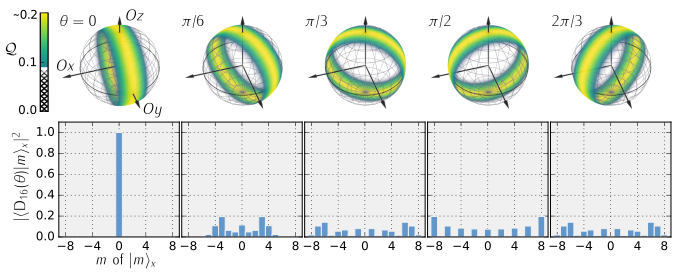
\includegraphics[scale=.65]{img/VD_evolution_of_dicke.pdf}
  \caption[Sequence of Dicke state evolution]{
  Sequence of the evolution of an unpolarized Dicke state of 16 qubits for $\theta=\{i\pi/6\}_{i=0}^4$.
  (sequence-above) Bloch spheres representing the Husimi quasi-probabilistic distribution $\mathcal{Q}$ of the state, see Appendix~\ref{app:husimi-representation} for details.
  (sequence-below) PDF of the $J_x$ positive-operator valued measure (POVM) for each step of the sequence.}
  \label{fig:vd-secuence-evo}
\end{figure}

In certain situations, it is better to use Eq.~\eqref{eq:bg-error-propagation-formula} rather than Eq.~\eqref{eq:bg-quantum-cr-bound} for calculating the achievable precision, since it gives the precision for a particular operator to be measured in an experimental setup.
This is reasonable, since in a typical experiment, only a restricted set of operators can be measured.
In this work, we will consider many-particle systems in which the particles cannot be accessed individually, and only collective quantities can be measured.
As we said, measuring the second moment of $J_x$ is a valid choice to estimate the rotation angle.
In the following equation, we show the error propagation formula when measuring the second moment of the $J_x$ total angular momentum component,
\be
  \varinv{\theta} = \frac{|\partial_{\theta} \expect{J_x}|^2}{\varian{J_x^2}}.
  \label{eq:vd-error-propagation}
\ee

Since Eq.~\eqref{eq:vd-error-propagation} is always smaller than $\qfi$, and as a consequence of Eq.~\eqref{eq:bg-entanglement-criterion-qfi}, if
\be
  \frac{|\partial_{\theta} \expect{J_x}|^2}{\varian{J_x^2}}\geqslant N
\ee
holds, then the system is entangled.
Hence again, entanglement is required for a large metrological precision.
Based on Eq.~\eqref{eq:bg-entanglement-depth-for-qfi}, we can bound the entanglement depth from below of the systems as follows.
Similarly to the previous paragraph, if for a quantum state
\be
  \frac{|\partial_{\theta} \expect{J_x}|^2}{\varian{J_x^2}}\geqslant kN
\ee
holds, then it is at least $(k+1)$-entangled.

\subsection{Precision based on the error propagation formula when $M=J_x^2$}
\label{sec:vd-evolution-of-the-expectation-values}
With the aim of obtaining the precision, Eq.~\eqref{eq:vd-error-propagation}, we will compute the dependence on $\theta$ of the expectation value of the operator $J_x$ and higher order moments.
We will use the Heisenberg picture, where the operators evolve in time while the state remains the same.
The operator $J_x$ can be written as a function of $\theta$ in the following way,
\be
  J_x(\theta) = e^{i \theta J_z} J_x(0) e^{-i \theta J_z} = J_x(0) \text{c}_\theta - J_y(0) \text{s}_{\theta},
\ee
where $J_l(0)$ for $l=x,y,z$ are the collective angular momentum operators at time equal zero.
We will denote them by $J_l$ from now on.
The notation for the trigonometric functions $\text{c}_\theta$ and $\text{s}_\theta$ was introduced in Section~\ref{sec:bg-metrology-with-almost-polarized}.

We need to compute the second and the fourth moments of $J_x$ as it is required by the Eq.~\eqref{eq:vd-error-propagation}.
But before any calculation we will make a simplifying assumption which turns out to be true in the most common situations.
The assumption is that both expectation values are even functions of $\theta$, so
\be
  \begin{split}
    \expect{J_x^2(\theta)} &=\expect{J_x^2(-\theta)}, \\
    \expect{J_x^4(\theta)} &=\expect{J_x^4(-\theta)}
  \end{split}
  \label{eq:vd-even-f-constraint}
\ee
holds.
This way we can omit the terms that are odd in $\theta$.
In Section~\ref{sec:vd-testing-with-experimental-data}, we will see that unitary dynamics of some experimentally prepared states have this property.
The assumption Eq.~\eqref{eq:vd-even-f-constraint} is needed to obtain a closed formula for the precision of the phase estimation.

The square of $J_x$ in the Heisenberg picture is written as
\be
  J_x^2(\theta)= J_x^2 \text{c}_\theta^2 + J_y^2 \text{s}_\theta^2
  - (J_xJ_y + J_yJ_x) \text{c}_\theta\text{s}_\theta.
  \label{eq:vd-evolution-of-jx2}
\ee
Hence, due to the first constraint of Eq.~\eqref{eq:vd-even-f-constraint} and Eq.~\eqref{eq:vd-evolution-of-jx2}, we require that
\be
  \expect{\{J_x,J_y\}} = 0.
  \label{eq:vd-init-2nd-constraint}
\ee
Eq.~\eqref{eq:vd-init-2nd-constraint} is based on expectation values of the initial state state.
The condition Eq.~\eqref{eq:vd-init-2nd-constraint} is fulfilled in a typical experiment.

As we have done with the expectation value of the square of $J_x$, now we  do the same for $J_x^4$.
This way one will be able to distinguish which other expectation value of combination of operators must vanish in order to have Eq.~\eqref{eq:vd-even-f-constraint} guarantied.
The fourth power of $J_x$ can be written in the Heisenberg picture as
\begin{multline}
  J_x^4(\theta)= J_x^4 \text{c}_\theta^4 + J_y^4 \text{s}_\theta^4
  + (J_x^2J_y^2 + J_xJ_yJ_xJ_y + J_xJ_y^2J_x + J_yJ_xJ_yJ_x + J_yJ_x^2J_y + J_y^2J_x^2) \text{c}_\theta^2\text{s}_\theta^2 \\
  -(J_x^3J_y+J_x^2J_yJ_x+J_xJ_yJ_x^2+J_yJ_x^3)\text{c}_\theta^3\text{s}_\theta
  -(J_xJ_y^3+J_yJ_xJ_y^2+J_y^2J_xJ_y+J_y^3J_x)\text{c}_\theta\text{s}_\theta^3.
\end{multline}
And again assuming that the expectation value of $J_x^4(\theta)$ must be an even function of $\theta$, we see that the terms multiplied by $\coss{\theta}^3\sins{\theta}$ and $\coss{\theta}\sins{\theta}^3$, respectively, must be zero.
So, the expectation value of $(J_x^3J_y+J_x^2J_yJ_x+J_xJ_yJ_x^2+J_yJ_x^3)$ and $(J_xJ_y^3+J_yJ_xJ_y^2+J_y^2J_xJ_y+J_y^3J_x)$ must vanish.
Hence, the second constraint of the Eq.~\eqref{eq:vd-even-f-constraint} can be fulfilled if
\be
  \begin{split}
    \expect{\big\{J_x^2 , \{ J_x,J_y\}\big\}}=0,\\
    \expect{\big\{J_y^2 , \{ J_x,J_y\}\big\}}=0.
  \end{split}
\ee

Finally, we can write the evolution of second and fourth moments of the $J_x$ operator as
\begin{align}
  \expect{J_x^2(\theta)}=\; &\expect{J_x^2} \text{c}_\theta^2 + \expect{J_y^2} \text{s}_\theta^2
  \label{eq:vd-evo-2nd-moment}\\
  \begin{split}
    \expect{J_x^4(\theta)}=\; &
    \expect{J_x^4}\text{c}_\theta^4 + \expect{J_y^4} \text{s}_\theta^4 \\
    & + \expect{\{J_x^2,J_y^2\}+\{J_x,J_y\}^2} \text{c}_\theta^2\text{s}_\theta^2.
  \end{split}
\end{align}
From here, we are able to write the evolution of the variance of the second moment when Eq.~\eqref{eq:vd-even-f-constraint} is fulfilled.
We obtain
\be
  \begin{split}
    \varian{J_x^2(\theta)} &= \expect{J_x^4(\theta)} -\expect{J_x^2(\theta)}^2 \\
    &= \expect{J_x^4}\text{c}_\theta^4 + \expect{J_y^4} \text{s}_\theta^4
    + \expect{\{J_x^2,J_y^2\}+\{J_x,J_y\}^2} \text{c}_\theta^2\text{s}_\theta^2
    - \big(\expect{J_x^2} \text{c}_\theta^2 + \expect{J_y^2} \text{s}_\theta^2\big)^2\\
    &= \big(\expect{J_x^4}-\expect{J_x^2}^2\big)\text{c}_\theta^4
    + \big(\expect{J_y^4}-  \expect{J_y^2}^2\big)\text{s}_\theta^4
    + \big(\expect{\{J_x^2,J_y^2\}+\{J_x,J_y\}^2} - 2 \expect{J_x^2}\expect{J_y^2}\big)
    \text{c}_\theta^2\text{s}_\theta^2\\
    &=\varian{J_x^2}\text{c}_\theta^4 + \varian{J_y^2} \text{s}_\theta^4+ \big(\expect{\{J_x^2,J_y^2\}+\{J_x,J_y\}^2} - 2 \expect{J_x^2}\expect{J_y^2}\big)\text{c}_\theta^2\text{s}_\theta^2.
  \end{split}
\ee

In order to compute the Eq.~\eqref{eq:vd-error-propagation}, we also need the modulus square of the derivative of the second moment of the $J_x$ operator.
Using Eq.~\eqref{eq:vd-evo-2nd-moment} for the expression of the evolution of the second moment, the numerator of Eq.~\eqref{eq:vd-error-propagation} follows
\be
  \begin{split}
    |\partial_\theta \expect{J_x^2(\theta)}|^2 & = |-2\expect{J_x^2}\text{c}_\theta\text{s}_\theta+2\expect{J_y^2}\text{c}_\theta\text{s}_\theta|^2\\
    & = 4\expect{J_y^2-J_x^2}^2\text{c}_\theta^2\text{s}_\theta^2.
  \end{split}
\ee

From the equations above directly follows expression for the precision of $\theta$,
\be
\begin{split}
  \varian{\theta} & = \frac{\varian{J_x^2}\text{c}_\theta^4 + \varian{J_y^2} \text{s}_\theta^4+ \big(\expect{\{J_x^2,J_y^2\}+\{J_x,J_y\}^2} - 2 \expect{J_x^2}\expect{J_y^2}\big)\text{c}_\theta^2\text{s}_\theta^2}
  {4\expect{J_y^2-J_x^2}^2\text{c}_\theta^2\text{s}_\theta^2}\\
  & = \frac{\varian{J_x^2}\text{t}_\theta^{-2} + \varian{J_y^2} \text{t}_\theta^2+ \expect{\{J_x^2,J_y^2\}+\{J_x,J_y\}^2} - 2 \expect{J_x^2}\expect{J_y^2}}
  {4\expect{J_y^2-J_x^2}^2}.
\end{split}
\label{eq:vd-result-before-simp}
\ee
To this calculations further computations follows mainly regarding to the following expectation value $\expect{\{J_x^2,J_y^2\}+\{J_x,J_y\}^2}$.
This calculus is left for the Appendix~\ref{app:simplification-of-4th-moments}.
Finally, the expression Eq.~\eqref{eq:vd-result-before-simp} can be written as
\be
  \varian{\theta} = \frac{\varian{J_x^2}\text{t}_\theta^{-2} + \varian{J_y^2} \text{t}_\theta^2 + 4\expect{J_y^2} - 3 \expect{J_z^2} - 2\expect{J_x^2}(1+\expect{J_y^2}) + 6\expect{J_xJ_y^2J_x}}
  {4\expect{J_y^2-J_x^2}^2}.
  \label{eq:vd-precision-as-theta}
\ee

We have verified the correctness of our analytic formula Eq.~\eqref{eq:vd-precision-as-theta} comparing it with a numerical simulation of the Eq.~\eqref{eq:vd-error-propagation} for the ground-state of $H=J_x^2+J_y$ for 6 qubits, $|\text{GS}\rangle$.
We computed the evolution of the expectation values of the second and the fourth moments of the operator $J_x$ for $\theta \in [0,\pi]$, for thousand of equidistant points, from which we obtained the bound, see Figure~\ref{fig:vd-evolution-of-precision}-(a).
Finally, we have also checked that the constraints assumed at the beginning of this section are fulfilled.
For that, we considered the range $\theta \in [-\pi,\pi]$ and we have computed the expectation values, see Figure~\ref{fig:vd-evolution-of-precision}-(b).
We can conclude saying that our formula Eq.~\eqref{eq:vd-precision-as-theta} reproduces exactly the evolution of the error propagation formula, Eq.~\eqref{eq:vd-error-propagation}.
\begin{figure}[htp]
  \centering
  \igwithlabel{(a)}{scale=.65}{img/VD_simulation.pdf}
  \igwithlabel{(b)}{scale=.65}{img/VD_parity_simulation.pdf}
  \caption[(a) Evolution of $\varinv{\theta}/N$. (b) Evolution of the expectation values]{
  (a) Evolution of the precision $\varinv{\theta}/N$ for 6 qubits based on the simulation of the system $\ket{\text{GS}}$ and its expectation values.
  The agreement with the Eq.~\eqref{eq:vd-precision-as-theta} is shown in the inset plot where the square of the difference between two approaches are plotted, the analytically obtained result and the simulation.
  The difference is more or less two orders of magnitude below the actual value for the relevant points, which is mainly because of computing the derivative near the points at which the expectation value $\expect{J_x^2}$ and the $\varian{J_x^2}$ are both close to zero.
  (b) With the system at hand, we verified the parity with respect to $\theta$ of the expectation values of the second and the fourth moment, so to fulfill the constraint Eq.~\eqref{eq:vd-even-f-constraint}.}
  \label{fig:vd-evolution-of-precision}
\end{figure}

\subsubsection{The optimal precision}
First of all, note that all the dependence on the phase shift $\theta$ is in the first two terms of the numerator of Eq.~\eqref{eq:vd-precision-as-theta}.
Hence, one can minimize the sum on the first two terms in order to find where the precision is best.
So it follows that for the optimal angle
\be
  \label{eq:vd-optimal-phase}
  \tan^2(\theta_{\text{opt}}) = \sqrt{\frac{\varian{J_x^2}}{\varian{J_y^2}}}
\ee
holds.
By substituting Eq.~\eqref{eq:vd-optimal-phase} into Eq.~\eqref{eq:vd-precision-as-theta}, we obtain the optimal bound as
\be
  \varian{\theta}_{\text{opt}} = \frac{\sqrt{\varian{J_x^2} \varian{J_y^2} } + 4 \expect{J_y^2} - 3 \expect{J_z^2} - 2\expect{J_x^2}(1+\expect{J_y^2}) + 6\expect{J_xJ_y^2J_x}}
  {4\expect{J_y^2-J_x^2}^2}.
  \label{eq:vd-precision}
\ee.

We conclude this section checking our bound for pure unpolarized Dicke state aligned with the $x$-axis, $\ket{\dicke{N}}_x$, whose precision bound is well known using the QFI for pure states Eq.~\eqref{eq:bg-qfi-for-pure-states},
\be
  \qfif{\ket{\dicke{N}}_x, J_z} = 4\varian{J_z}_{\ket{\dicke{N}}_x}=\frac{N(N+2)}{2}.
  \label{eq:vd-qfi-for-pure-dicke}
\ee
With this aim we compute all the expectation values needed for the Eq.~\eqref{eq:vd-precision} which almost all of them are trivial, $\expect{J_xJ_y^2J_x}=\expect{J_x^4}=\expect{J_x^2}=0$ since the state is an eigenstate of $J_x$ with an eigenvalue zero.
The last expectation value is obtained as
\be
  \expect{J_y^2} = \expect{J_z^2} = \frac{N (N+2)}{8}.
  \label{eq:vd-2moment-pure-dicke}
\ee
Note that for the Eq.~\eqref{eq:vd-2moment-pure-dicke} we use that the state is invariant under rotations over the $x$-axis, the sum of all the second moments must give $\expect{\bs{J}^2} = \frac{N (N+2)}{4}$, and $\expect{J_x^2}=0$.
Hence, the Eq.~\eqref{eq:vd-2moment-pure-dicke} holds.

From the Eq.~\eqref{eq:vd-2moment-pure-dicke} using the expression for the optimal precision Eq.~\eqref{eq:vd-precision} and substituting all the terms that are zero, one arrives at the following formula for the precision of the phase shift for a pure unpolarized Dicke state,
\be
  \varian{\theta}_{\text{opt}} = \frac{2}{N(N+2)},
\ee
which coincides exactly with the inverse of the quantum Fisher information for such state Eq.~\eqref{eq:vd-qfi-for-pure-dicke} \cite{Luecke2011}.
Hence for the ideal Dicke state, the Cramér-Rao bound Eq.~\eqref{eq:bg-quantum-cr-bound} is saturated, which means that estimating the phase shift $\theta$ using the measurement of $\expect{J_x^2}$ is optimal.
Based on Eq.~\eqref{eq:vd-optimal-phase}, we add that the optimal angle for the ideal Dicke state is $\theta_{\text{opt}}=0$.

\subsection{Testing the formula against some known states}
\label{sec:vd-comparison-with-qfi}

In this section, we will compare our criteria based on few expectation values against the corresponding quantum Fisher information obtained for some known states.
We find that our formula gives a good lower bound on the quantum Fisher information, which is the best achievable precision when any measurement is allowed.
However note that the Cramér-Rao bound might be impractical.

Let us consider first the spin-squeezed states.
Those states will be defined as the ground states $\ket{\text{GS}}_\lambda$ of the following Hamiltonian, called the spin-squeezing Hamiltonian
\be
  H_\lambda = J_x^2 - \lambda J_y,
  \label{eq:vd-ss-hamiltonian}
\ee
see Appendix~\ref{app:spin-squeezing-hamiltonian}.
For $\lambda>0$, the ground state is unique, and it is in the symmetric subspace.
Hence, we can restrict our attention to this subspace for our computations, and hence we can model larger systems.
For $\lambda\rightarrow\infty$, the ground state is the totally polarized state in the $y$-direction Eq.~\eqref{eq:bg-totally-polarized}.
And for $\lambda\rightarrow 0^{+}$, it is the Dicke state Eq.~\eqref{eq:vd-unpolarized-dicke}.
Note that for $\lambda=0$ the eigenvalue is degenerate, so there are more than one ground states.
On the other hand, we still can use limit in which $\lambda$ tends to zero from the positive axis to arrive at the Dicke state.
Figure~\ref{fig:vd-comparing-the-bounds}-(a) shows the sensitivity we obtained together with the QFI for the same states.
Our bound is close to the QFI when the state is well polarized.
It also coincides with the bound in the $\lambda\rightarrow 0^{+}$ limit, when the ground state is close to the unpolarized Dicke state.
\begin{figure}[htp]
  \centering
  \igwithlabel{(a)}{scale=.65}{img/VD_against_spsq.pdf}
  \igwithlabel{(b)}{scale=.65}{img/VD_against_therm.pdf}
  \caption[Comparing our bound and known QFIs.]{
  Comparison between our formula for the precision and the QFI for different states. (a) Comparison with ground states of $H_\lambda$. (b) Comparison with thermal mixture of Dicke states.}
  \label{fig:vd-comparing-the-bounds}
\end{figure}

The second family of states we use to test our formula are the Gaussian mixture of Dicke states around the unpolarized Dicke state,
which have the following form as function of $T$ as
\be
  \rho_{T} \propto \sum_{n=0}^{N} e^{- \frac{(n+N/2)^2}{T}} \ket{\dicke{N,n}}_x\bra{\dicke{N,n}}_x
\ee
for even $N$, where $\ket{\dicke{N,n}}$ is defined in Eq.~\eqref{eq:app-definition-of-dicke-states}.
It can be used to model a noisy or thermal unpolarized Dicke state.
For $T=0$, we obtain the pure unpolarized Dicke state.
For $T>0$, other symmetric Dicke states in the vicinity of the unpolarized one are also populated.
The result can be seen in Figure~\ref{fig:vd-comparing-the-bounds}-(b).
Again, our bound seems to be quite close to the corresponding QFI.

Note also that in Figure~\ref{fig:vd-comparing-the-bounds}, based on Eq.~\eqref{eq:bg-entanglement-depth-for-qfi}, if the bound turns to be greater than $k$ integer, then a metrologically useful $(k+1)$-particle entanglement is detected in the system.
Note that this is true whenever $k$ is a divisor of $N$, or $k\ll N$.

Although showing how the optimal precision formula behaves compared with the quantum Fisher information for those two families of states, we will now prove that they indeed they fulfill the constraints appearing in Eq.~\eqref{eq:vd-even-f-constraint}.
Hence, we compute the Eq.~\eqref{eq:vd-even-f-constraint} for the spin-squeezed states $\ket{\text{GS}}_{\lambda}$.
For that it is enough to know that since those states are non-degenerate eigenvalue must preserve the symmetries of the Hamiltonian.
In this case, the Hamiltonian Eq.~\eqref{eq:vd-ss-hamiltonian} is invariant under $x\leftrightarrow -x$ and $z\leftrightarrow -z$, thus it must be invariant under $r\pi$ angle rotations under the $y$-axis for $r$ integer, for more references about symmetries in quantum mechanics see Refs. \cite{Sakurai2010, Cohen-Tannoudji1977}.
Hence, we can write for the evolution of the expectation value of any power $m$ of $J_x$ such that
\be
  \tr(e^{+i\theta J_z}J_x^m e^{-i\theta J_z} \rho_{\lambda}) = \tr(e^{+i\theta J_z}J_x^m e^{-i\theta J_z} e^{-i r\pi J_y}\rho_{\lambda}e^{+i r\pi J_y}),
\ee
where $\rho_{\lambda}=\ketbra{\text{GS}}{\text{GS}}_{\lambda}$.
Then for the case $r=1$, we can use the cyclic property of the trace to arrive at
\be
\begin{split}
  \tr(e^{+i\pi J_y}e^{+i\theta J_z}J_x^m e^{-i\theta J_z} e^{-i\pi J_y}\rho_{\lambda}) & =
  \tr(e^{+i \theta (-1)J_z}(-1)^m J_x^m e^{-i\theta (-1) J_z}\rho_{\lambda})\\
  & = \tr(e^{-i \theta J_z}(-1)^m J_x^m e^{+i\theta J_z}\rho_{\lambda}),
\end{split}
\ee
or equivalently
\be
  \expect{J_x^m(\theta)}_{\rho_\lambda}=\expect{(-1)^m J_x^m(-\theta)}_{\rho_\lambda},
\ee
which implies that for even $m$, and specially for $m=2,4$, the expectation values are an even function of $\theta$, and that for odd $m$ the expectation values are odd functions of $\theta$, which proves the Eq.~\eqref{eq:vd-even-f-constraint} for the present case.

On the other hand, the eigenstates of the thermal state $\rho_T$ are simultaneously eigenstates of $J_x$, and hence the state invariant under rotations around the $x$-axis.
Which still holds for the entire state, since it is a statistical mixture of states invariant under rotations around the $x$-axis.
Moreover, it is also invariant for the case in which the state is rotated around the $x$-axis by $\pi$ angle.
Hence, we have for the evolution of the expectation values of $J_x^m$ that
\be
  \tr(e^{+i\theta J_z}J_x^m e^{-i\theta J_z}\rho_T) = \tr(e^{+i\theta J_z}J_x^m e^{-i\theta J_z} e^{-i \pi J_x} \rho_T e^{+i \pi J_x})
\ee
for any $m$.
Finally, using again the cyclic properties of the trace, we flip the signs of the of angular momentum components orthogonal to $J_x$, so in this case $J_y \rightarrow - J_x$ and $J_z \rightarrow -J_z$, and we arrive at
\be
  \tr(e^{+i \pi J_x} e^{+i\theta J_z}J_x^m e^{-i\theta J_z} e^{-i \pi J_x} \rho_T) =  \tr(e^{-i\theta J_z}J_x^m e^{+i\theta J_z} \rho_T).
\ee
We conclude that for the thermal state this case all the moments of the $J_x$ operator are even functions of $\theta$ for the thermal state, i.e., $\expect{J_x^m(\theta)}_{\rho_{T}}=\expect{J_x^m(-\theta)}_{\rho_{T}}$, which proves that the Eq.~\eqref{eq:vd-even-f-constraint} holds for this case too.

\subsection{Using our method with real experimental data}
\label{sec:vd-testing-with-experimental-data}

In reference \cite{Luecke2014}, a state is produced in the laboratory with the proper characteristics of an unpolarized Dicke state, small variance in one direction, say $x$, and a very large variance in the perpendicular directions to the $x$-axis.
In the cited experiment with $N$ qubits, it is possible to determine the operator $J_x$ as the population imbalance of the two levels as
\be
  J_x = \frac{1}{2}(N_{1,x}-N_{0,x}),
\ee
where $N_{m,x}$ is the number of particles in the state $\ket{m}_x$.
Hence, measuring the population imbalance and collecting the statistics of the measurements, the expectation values of all moments of $J_x$ can be obtained.
In practice, it is possible to measure the lower order moments like $\expect{J_x^2}$ and $\expect{J_x^4}$, while higher order moments need too many repetitions of the experiment to collect enough statistics.

The other two global operators $J_y$ and $J_z$ are obtained by rotating the system using a $\frac{\pi}{2}$ microwave coupling pulse before the measurement of the population imbalance.
Whether $J_y$ or $J_z$ is obtained depends on the relation between the microwave phase and the phase of the initial BEC.
The condensate phase represents the only possible phase reference in analogy to the local oscillator in optics.
Intrinsically, it has no relation to the microwave phase, such that it homogeneously average over all possible phase relations.
From another point of view, one can also say that the fluctuation of the magnetic field results in a random rotation of the spin around the $z$-axis.
Hence, what is obtained in this case is
\be
  J_\alpha = \sin(\alpha) J_y + \cos(\alpha) J_z,
\ee
where $\alpha$ is an angle, and we need to consider the average over all possible angles.
Effectively, the state has the following form
\be
  \rho = \frac{1}{2\pi}\int e^{-i\alpha J_x} \rho_0 e^{i\alpha J_x}\, \text{d}\alpha,
  \label{eq:vd-rotational-invariant-state}
\ee
where $\rho_0$ is what we would obtain if we would have access to the phase reference.
Note that the integration over the rotation angle $\alpha$ does not create entanglement.
If the state $\rho$ is entangled then $\rho_0$ has to be also entangled.

Let us see the consequences of our state having the form  Eq.~\eqref{eq:vd-rotational-invariant-state}.
For the density matrix $\rho$, since it is invariant under rotations around the $x$-axis, we have
\be
  \expect{J_\alpha^m}=\expect{J_y^m}=\expect{J_z^m}
\ee
for all $m$.
Hence the expectation values of $\expect{J_y^m}$ and $\expect{J_z^m}$ can be obtained from the statistics of measuring $J_\alpha$.
Moreover, for states of the form Eq.~\eqref{eq:vd-rotational-invariant-state} the unitary dynamics will fulfill the condition Eq.~\eqref{eq:vd-even-f-constraint}.

There is a single remaining term in the expression for the achievable precision Eq.~\eqref{eq:vd-precision}, the expectation value for $\expect{J_xJ_y^2J_x}$, which can be bounded as
\be
\begin{split}
  \expect{J_xJ_y^2J_x} &= \frac{\expect{J_x (J_y^2 + J_z^2)J_x}}{2}
  =\frac{\expect{J_x (J_x^2 + J_y^2 + J_z^2 )J_x} - \expect{J_x^4}}{2} \\
  & \leqslant \frac{N(N+2)}{8} \expect{J_x^2} - \frac{\expect{J_x^4}}{2},
\end{split}
\label{eq:vd-simplification-of-last-4th-moment}
\ee
where the last inequality is due to that for all states $\expect{\bs{J}^2}\leqslant \mathcal{J}_{N/2}$, see Eq.~\eqref{eq:app-maximum-total-angular-momentum}, while symmetric states saturate the inequality in Eq.~\eqref{eq:vd-simplification-of-last-4th-moment}.
Note that obtaining $\expect{J_xJ_z^2J_x}$ can be hard experimentally.
In any case, this simplification can only make our estimation of the precision worse while for symmetric states the equality holds.
Hence, the lower bound for the achievable precision can be written as
\be
  \varian{\theta}_{\text{opt}} \leqslant \frac{\sqrt{\varian{J_x^2} \varian{J_y^2} } + \expect{J_y^2} + \frac{3N(N+2)-8}{4} \expect{J_x^2} - 2\expect{J_x^2}\expect{J_y^2} - 3\expect{J_x^4}}
  {4\expect{J_y^2-J_x^2}^2},
\ee
where some terms were reordered and further simplified.

It is worth to study the case appearing in Ref.~\cite{Krischek2011} and apply our methods such that we obtain conclusions about the metrological usefulness of the state.
The system under consideration has around $N=7900$.
Note that using the expectation value of the particle number, in our case $\expect{N}=7900$, cannot overestimate any lower bound on the precision.
For a discussion about entanglement criteria in systems with particle number fluctuations see Ref.~\cite{Hyllus2012a}.
The measured data for the system yields
\be
\begin{aligned}
  \expect{J_x^2} & = 112 \pm 31, \\
  \expect{J_x^4} & = 40 \times 10^3 \pm 22 \times 10^3,
\end{aligned}
\quad
\begin{aligned}
  \expect{J_y^2} & = 6 \times 10^6 \pm 0.6 \times 10^6, \\
  \expect{J_y^4} & = 6.2 \times 10^{13} \pm 0.8 \times 10^{13}.
\end{aligned}
\label{eq:vd-experimental-values}
\ee
Hence, we obtain the maximum precision as
\be
  \frac{(\Delta \theta)^{-2}_{\text{opt}}}{N} \geqslant 3.7 \pm 1.5.
  \label{eq:vd-precision-for-experiment}
\ee
The statistical uncertainties of Eqs.~\eqref{eq:vd-experimental-values} and \eqref{eq:vd-precision-for-experiment} have been obtained through bootstraping, while the direct substitutions of expectation values would yield to 3.3 of gain over the shot-noise limit $\varinv{\theta}=N$.
Based on Eq.~\eqref{eq:bg-entanglement-criterion-qfi}, this proves the presence of metrologically useful entanglement \cite{Pezze2009}.
Based on Eq.~\eqref{eq:bg-entanglement-depth-for-qfi}, it even demonstrated that the quantum state had metrologically useful 4-particle entanglement.
Assuming an error of a standard deviation, Eq.~\eqref{eq:vd-precision-for-experiment} still proves 3-particle entanglement.

Next we plot the value for the precision substituting directly the experimental data into Eq.~\eqref{eq:vd-precision-as-theta}, see Figure~\ref{fig:vd-precision-theta-experiment}.
Since we cannot obtain the expectation value $\expect{J_xJ_y^2J_x}$ we approximate it with the right-hand side of Eq.~\eqref{eq:vd-simplification-of-last-4th-moment}.
With that we underestimate $\varinv{\theta}$.
\begin{figure}[htp]
  \centering
  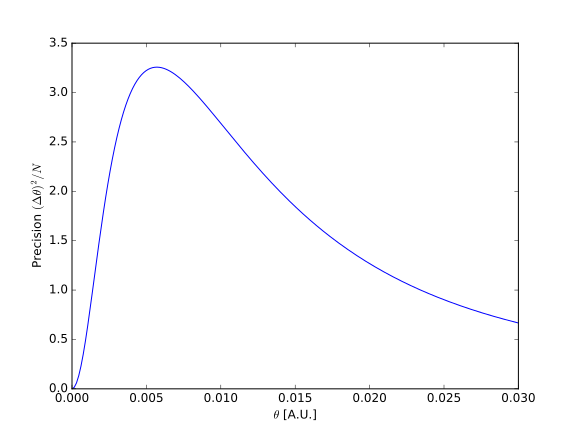
\includegraphics[scale=.65]{img/VD_precision_theta.pdf}
  \caption[Evolution in $\theta$ of the precision.]{
  (solid) The precision as a function of the parameter $\theta$ given by Eq.~\eqref{eq:vd-precision-as-theta} varies through the evolution.
  Note that for the initial moment the precision is zero.
  (dashed) We highlight where the precision reaches its maximum at $\theta \approx 0.0057$.
  (gray-area) It represent the region where the precision is below the shot-noise limit.}
  \label{fig:vd-precision-theta-experiment}
\end{figure}

Thus, we could detect metrological usefulness by measuring the second and fourth moments of the collective angular momentum components.
For future applications of our scheme, it is important to reduce further the number of quantities we need to obtain a lower bound for the precision.
In practice, one can easily avoid the need for determining $\expect{J_y^4}$.
Note that if we measure $J_y$ then the distribution of the values obtained is strongly non-Gaussian.
The values $\pm N/2$ appear most frequently, and the value 0 appears least frequently \cite{Luecke2011}.
See also the distribution of a pure Dicke state when $\theta=\pi/2$ in the Figure~\ref{fig:vd-secuence-evo}.
The state has more overlap with the eigenstates of the edges than in the middle.
Based on $\expect{AB}\leqslant\lambda_{\max}(A)\expect{B}$, where $\lambda_{\max}(A)$ is the largest eigenvalue of $A$, for two commuting positive-semidefinite observables,
\be
  \expect{J_y^4}\leqslant\frac{N^2}{4}\expect{J_x^2}.
\ee
Since even for a noisy Dicke state $\expect{J_y^2}$ is very large, the above equation is a very good upper bound.
Substituting it into the Eq.~\eqref{eq:vd-precision}, we will underestimate $\varinv{\theta}$.

It is also possible to approximate $\expect{J_x^4}$ with $\expect{J_x^2}$ in the sense that it is small and that mainly its value comes from technical noise,
\be
  \expect{J_x^4} \approx \beta \expect{J_x^2}^2.
\ee
This approximation, even if it is not a strict bound on the precision, can be very useful in order to characterize the metrological usefulness of the state based only on second statistical moments of only two angular momentum components, namely $\expect{J_y^2}$ and $\expect{J_x^2}$.
Those two expectation values are related with how  thin is the state in one direction and how wide in the perpendicular ones.
So in this case we use $\beta=3$ assuming that the distribution function has a Gaussian shape.

From these considerations we are able to write a second bound with fewer expectation values for the optimal precision such that
\be
  \varian{\theta}_{\text{opt}} \leqslant \frac{\expect{J_y^2} + \frac{3N(N+2)-8}{4} \expect{J_x^2} + \Big(\sqrt{\frac{N^2}{2\expect{J_y^2}}-2} - 2 \Big) \expect{J_y^2}\expect{J_x^2} - 9\expect{J_x^2}^2}
  {4\expect{J_y^2-J_x^2}^2}.
  \label{eq:vd-precision-bound-for-second-moments}
\ee
We have used this formula to compute the bound for the optimal precision with the measured data shown on Eq.~\eqref{eq:vd-experimental-values}, $(\Delta \theta)^{-2}_{\text{opt}} \geqslant 2.9N$, see Figure~\ref{fig:vd-experimental}.
It turns out that even this way, 3-particle metrologically useful entanglement is detected.
\begin{figure}[htp]
  \centering
  \igwithlabel{(a)}{scale=.65}{img/VD_exper_contour.pdf}
  \igwithlabel{(b)}{scale=.65}{img/VD_exper_slice.pdf}
  \caption[(a) Precision bound for $\expect{J_y^2}$ and $\expect{J_x^2}$. (b) Slice in constant $\expect{J_y^2}$.]{
  (a) Precision bound as a function of $\expect{J_y^2}$ and $\expect{J_x^2}$.
  The expectation value $\expect{J_y^2}$ is normalized with $\mathcal{J}_{N/2}$.
  (solid) Different boundaries for metrologically useful entanglement depths.
  (cross) Experimental data.
  (blue-ellipse) Region with one $\sigma$ confidence from the experimental data.
  (vertical-dashed) Constant $\expect{J_y^2}$ cross section plotted in (b).
  (b) Constant $\expect{J_y^2}$ cross section for the precision bound.
  (solid) Precision bound based on the Eq.~\eqref{eq:vd-precision-bound-for-second-moments}.
  One can see that decreasing further the uncertainty in $\expect{J_x^2}$ can improve the bound significantly.
  (white-point) Experimental data with the corresponding errors bars.
  (gray-area) Shot-noise limit.
  The point is slightly below the 4-particle entanglement level.}
  \label{fig:vd-experimental}
\end{figure}

In Figure~\ref{fig:vd-experimental}-(a), we show the two-dimensional plot which is obtained based on these considerations.
The regions with various levels of multipartite entanglement ca clearly be identified.
The ideal Dicke state corresponds to the bottom-right corner, where $\expect{J_x^2}=0$ and $\expect{J_y^2}$ is largest.
In Figure~\ref{fig:vd-experimental}-(b), the cross section of the two-dimensional plot is shown.

Summarizing, we have shown that characterizing the metrological usefulness of noisy Dicke states can be done using few experimental data.
Furthermore, the precision bound is computed with the expectation values of the second and fourth moments of the angular momentum in the directions perpendicular to the magnetic field.
We have shown some simplifying techniques which reduce the experimental efforts needed to characterize the state. 

\section[Witnessing metrologically useful entanglement]
{Witnessing metrologically useful {\color{grey} X} entanglement}
\thiswatermark{\put(1,-282){\color{l-grey}\rule{84pt}{88pt}}
\put(84,-282){\color{grey}\rule{410pt}{88pt}}}


\lettrine[lines=2, findent=3pt,nindent=0pt]{T}{ypically}, one has not access to the density matrix of the system been used for metrology or for other quantum process.
Moreover, for systems on which the particle number is very large, this is the case when one wants to do metrology with quantum states, the details of the density matrix are forbidden by practical reasons.
Since the quantum Fisher information is based on the complete knowledge of the density matrix, shortcuts to avoid the complete tomography must be developed as we have had shown one practical case on the previous chapter.
In this chapter, we obtain a general procedure to get an optimal bound for the quantum Fisher information based on as many expectation values of the initial state as one is ready to measure.
Two main features are worth to mention again.
First, in general this method gives us an optimal tight bound.
Last but not least, the bound is based on the expectation values of the initial state only, so it is not necessary to perform an evolution of the state to estimate how well will it behave.
This is in contrast to other approaches one can find in the literature, an it is a time saving concept.

The figure of merit of bounds from below for the quantum Fisher information based on expectation values of the initial state is the following,
\be
  \qfi [\rho,J_z] \geq \frac{\expect{J_x}^2}{\varian{J_y}}.
\ee
where the state is polarized along the $x$-axis and the variance of the $J_y$ operator is smaller than the standard.
On the previous chapter we also have shown one of these bound specifically designed for unpolarized Dicke states.

Homogeneous magnetometry, $\bs{B} = B\bs{k}$ where $B$ is constant in time.

Section~[REF], see magnetometry, generator $J_z$.

Quantum Fisher information $\qfi [\rho, J_z]$.

\subsection{Minimum of a convex function of the state given some expectation values}

Convex function of state, $g(\rho)$.

Which is the lowest possible value of $g(\rho)$ for a state where some expectation values of $\{W_{i}\}_{i=1}^M$ operators, $w_i = \tr(\rho {W}_i)$ are known?

Such bound is defined in a way to fulfill the following inequality,
\be
  g(\rho) \geq \mathcal{B}_{g}(w_1,w_2,...) := \big\{\min_{\rho}g(\rho) \,|\,  \{w_i = \tr(\rho {W}_i)\}_{i=1}^M\big\}.
\ee
When computing this bound we will require to this to be as tight as possible.

For this purpose we simplify our discourse to one expectation value and therefore one observable, $w = \tr(\rho W)$.
Later we will extend our results to the multi-parameter case.

Notice that the tightest bound from below on of such a function $g(\rho)$ is convex too on the expectation values\ie $\mathcal{B}_g(w)$ is convex if $g(\rho)$ is convex.
This is shown in the following way,

Therefore, theory tells us that we can use the Legendre transform to get rid of the state preserving all the necessary information to reconstruct the $\mathcal{B}_{g}$ bound from the expectation values, this can be found on the work of Prof.~G\"uhne and Prof.~Werner Reference~\citep{XXX} and for a brief description of the properties of the Legendre transform see Appendix~\ref{ap:}.
In this case the Legendre transform can be written in the following way,
\be
  \hat{g}(rW) = \sup_{\rho}\{ r\expect{W}_{\rho}-g(\rho)\}.
\ee

Now we have the Legendre transform, we recover the bound from below of $g(\rho)$ as
\be
  \label{eq:lt-generic-bound-for-convex-func}
  \mathcal{B}_g (w) = \sup_{r}\big\{rw-\sup_{\rho}\{r\expect{W}_{\rho}-g(\rho)\}\big\}.
\ee
To clarify, notice that the $\rho$ appearing on the inner maximization is not related with the one appearing on $g(\rho)$ that is bounded by $\mathcal{B}_g$ but a variable state for the maximization.

The Equation~(\ref{eq:lt-generic-bound-for-convex-func}) has been applied on entanglement measures, when $g(\rho)$ is defined using the convex roof construction\ie the function $g(\rho)$ is extended from the well defined region, namely the region of pure states, to the mixed states using the convex roof construction.
For illustrative purposes the convex roof of a function defined for pure states is the following,
\be
  g(\rho) = \inf_{\{p_k,\ket{\phi_k}\}}\big\{\sum_{k}p_k g(\ket{\phi_k})\big\}
\ee
for any decomposition $\rho=\sum_k p_k \ketbra{\phi_k}{\phi_k}$
In this case the Equation~(\ref{eq:lt-generic-bound-for-convex-func}) can be further simplified.
Let us focus by now on the inner maximization,
\be
\begin{split}
  \hat{g}(rW) & = \sup_{\rho}\{r\expect{W}_\rho - g(\rho)\} \\
  &=\sup_{\rho}\Big\{r\expect{W}_\rho - \inf_{\{p_k,\ket{\phi_k}\}}\big\{\sum_{k} p_k g(\ket{\phi_k})\big\} \Big\} \\
  &=\sup_{\{p_k, \ket{\phi_k}\}} \Big\{ \sum_k p_k r\expect{W}_{\ket{\phi_k}} - \inf_{\{p_k, \ket{\phi_k}\}} \big\{\sum_k p_k g(\ket{\phi_k}) \big\}  \Big\} \\
  &=\sup_{\{p_k, \ket{\phi_k}\}} \Big\{ \sum_k p_k \big\{ r\expect{W}_{\ket{\phi_k}} - g(\ket{\phi_k}) \big\} \Big\} \\
  &=\sup_{\ket{\psi}} \big\{ r\expect{W}_{\ket{\psi}} - g(\ket{\psi}) \big\}.
\end{split}
\ee
So now we have restricted the maximization to only pure states as it is shown on Reference~\citep{XXX}.

One the other hand, one can find different definitions of the QFI in the literature.
Among those definitions, there is one that defines the QFI as the convex roof of four times the variance of the generator of the unitary phase shift that suffers the state \citep{XXX}.
This can be written in the following way,
\be
  \qfi[\rho, G] = \inf_{\{p_k, \ket{\phi_k}\}}4\sum_k p_k (\Delta G)_{\ket{\phi_k}}^2
\ee

Even further simplification can be achieved for quantum Fisher information,
\be
\begin{split}
  \hat{\qfi}(rW) &= \sup_{\ket{\psi}}\big\{r\expect{W}_{\ket{\psi}}-4\varian{J_z}_{\ket{\psi}}\big\} \\
  &= \sup_{\ket{\psi}} \big\{ r\expect{W}_{\ket{\psi}}-4\expect{J_z^2}_{\ket{\psi}} + 4\expect{J_z}^2_{\ket{\psi}} \big\} \\
  &= \sup_{\ket{\psi}} \{\expect{rW-4J_z^2}_{\ket{\psi}} +
  \expect{2J_z}^2_{\ket{\psi}}\},
\end{split}
\label{eq:lt-legendre-of-qfi}
\ee
which is clearly a second order maximization over pure states.

With that at hand we are able to prove the following observation: the Legendre transform of the highest lower bound of the quantum Fisher information when the expectation value of some operator $W$ is known, can be written as the maximization over some parameter $\mu$ of the highest eigenvalue  $\lambda_{\max}(rW-4(J_z-\mu)^2)$.
This can  be expressed as follows,
\be
  \hat{\qfi}(rW) = \sup_\mu \{\lambda_{\max} (rW-4(J_z-\mu)^2)\},
\ee
where at the maximum the derivative with respect to $\mu$ must be zero for this quadratic function on the state.
Hence, the value of $\mu$ will coincide with the expectation value on the optimal state $\expect{J_z}_{\psi}$
Therefore, the finding of the optimal parameter $\mu$ is delimited to the range defined by $[\expect{J_z}_{\min},\expect{J_z}_{\max}]$.
For qubits this means that we have to perform a search for $\mu_{\text{opt}}$ in between $-N/2\leq \mu \leq N/2$.

Another way of getting the result of the maximization for the second order equation is parameterizing the eigenstate with the maximum eigenvalue of the operator $rW-4(J_z-\mu)^2$, so we get $\ket{\phi_{\max}(\mu)}$, and finally computing the expectation values of Equation~(\ref{eq:lt-legendre-of-qfi}) and maximizing it.

With this a tight bound from below for the quantum Fisher information can be found when the expectation value of an observable, say $W$, is known as follows,
\be
  \mathcal{B}_{\mathcal{F}}(w) = \sup_r \big\{ rw - \sup_{\ket{\psi}} \{\expect{rW-4J_z^2} + \expect{2J_z}^2\}\big\}.
\ee
One may notice that the inner maximization is a second order maximization.

This can be extended for several observables as follows
\be
  \mathcal{B}_{\mathcal{F}}(w_1,w_2,...) = \sup_{\bs{r}} \big\{ \bs{rw} - \sup_{\ket{\psi}} \{\expect{\bs{rW}-4J_z^2} + \expect{2J_z}^2\}\big\},
\ee
where $\bs{r}=(r_1,\dots,r_m)$ is the vector form and the same applies to $\bs{w}$ and the operators set $\bs{W}$.
The contraction of two of those vectors must be seen as a scalar product\ie $\bs{rW}=\sum r_iW_i$ where $W_i$ is the corresponding $i^{\text{th}}$ operator of $\bs{W}$.

\begin{figure}
  \centering
  \igwithlabel{(a)}{scale=.65}{img/plots/LT_fidGHZ.pdf}
  \igwithlabel{(b)}{scale=.65}{img/plots/LT_fidDicke.pdf}
  \caption{(a) Analytical solution of the bound $\mathcal{B}_{\mathcal{F}}$ for different values of the fidelity with respect to the GHZ state. (b) Numerical results for the minimum quantum Fisher information as a function of the fidelity with respect of unpolarise Dicke states perpendicular to the magnetic field, $|\text{D}_N^0\rangle$. (blue-line) For systems with 4 particles and (red-dashed) for system with 8 particles. One may notice that when the fidelity is at its maximum the bound approaches to 0.5 as it is the quantum Fisher information for large particle number.}
  \label{fig:vd-secuence-evo}
\end{figure}

\begin{figure}
  \centering
  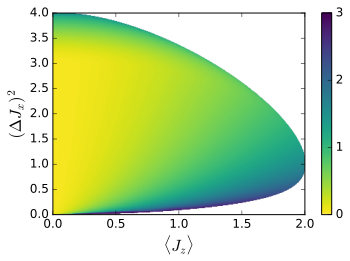
\includegraphics[scale=.65]{img/plots/LT_spsq2d_4.pdf}
  \caption{We show as a function of the expectation value, $\expect{J_y}$, and the variance in the perpendicular direction, $\varian{J_x}$, the minimum sensitivity for a 4-qubit system.
  (hatched) The physically forbidden region is indicated. (M,T,S,D) Those points indicate where the mixed state (), the totally polarized state (), the single state and the unpolarized Dicke state would be located. (W) on this line sit any of the states which is a mixture between the completely mixed state of the symmetric subspace and the singlet state among others, for instance the completely mixed state of the whole Hilbert space. (dashed) It indicates the shot-noise threshold where below it non-classical sensitivities can be achieved.}
  \label{fig:lt-spsq2d-4}
\end{figure}

\begin{figure}
  \centering
  \includegraphics[scale=.65]{img/plots/LT_edge_diff.pdf}
  \caption{Difference between the bound of Pezze-Smerzi and the optimal bound for the quantum Fisher information normalized by the value of the optimal bound itself for the bosonic ground states of $H=J_x^2-\lambda J_y$ for $\forall \lambda \in [0,\infty)$.
  From dark to lighter colors (line, point, dash-point, dashed, pointed, line), results for different particle numbers, $N=4,6,10,20,1000$ respectively.
  Heuristically speaking, one can say that for large particle number the difference is biggest when the polarisation is around two thirds of the maximal polarisation and that this difference is about $2.6\%$.}
  \label{fig:lt-edge-diff}
\end{figure}

\begin{figure}
  \centering
  \igwithlabel{(a)}{scale=.65}{img/plots/LT_spsq_scaling_1.pdf}
  \igwithlabel{(b)}{scale=.65}{img/plots/LT_spsq_scaling_2.pdf}
  \caption{}
  \label{fig:lt-spsq-scaling}
\end{figure}

\begin{figure}
  \centering
  \includegraphics[scale=.65]{img/plots/LT_dicke_edge.pdf}
  \caption{The numerics shows us a tiny region the symmetric system surpassing the shot-noise threshold.}
  \label{fig:vd-secuence-evo}
\end{figure}

\begin{figure}
  \centering
  \includegraphics[scale=.65]{img/plots/LT_dicke_7900_asymp.pdf}
  \caption{Secuence of the evolution of an unpolarized Dicke state of 16 qubits for $\Theta=\{i\pi/6\}_{i=0}^4$. Bloch spheres representing the Hirusi distribution of the state, and below PDF of the $J_x$ POVM for each step of the secuence}
  \label{fig:vd-secuence-evo}
\end{figure}

\lettrine[lines=2, findent=3pt, nindent=0pt]{I}{n} this chapter, one of the most fundamental two-parameter estimation tasks in magnetometry is considered, namely gradient magnetometry.
We will add the gradient of the magnetic field as the second parameter beside the constant (homogeneous) part of the field.
While most works in magnetometry with a single ensemble focus only on the determination of the strength and direction of magnetic field, certain measurement schemes for the gradient have already been proposed and tested experimentally.
Some schemes use an imaging of the ensemble with a high spatial resolution, however, they do not count as single-ensemble methods in the sense we use this expression in our paper, since in this case not only collective observables are measured  \cite{Vengalattore2007,Zhou2010,Koschorreck2011}.
There is a method based on collective measurements of the spin length of a fully polarised ensemble \cite{Behbood2013}.
Finally, there is a scheme  based on many-body singlet states described in Ref.~\cite{UH13}.
Our paper provides precision bounds for that scheme, while expanding the quantum states considered to several interesting quantum states, including those that are not invariant under homogeneous fields.

We can write the field at the atoms, situated along 1-dimensional $y=z=0$
degree of freedom, as
\begin{equation}
\bs{B}(x,0,0)=\bs{B}_0 +x \bs{B}_1 + O(x^2),
\end{equation}
where we will neglect the terms of order two or higher.
We will consider the magnetic field pointing along the $z$ direction,
$\bs{B}_0=B_0 \cdot (0,0,1)$ and
$\bs{B}_1=B_1 \cdot (0,0,1)$.
For this configuration, due to the Maxwell equations, with no currents or changing electric fields, we have
\begin{eqnarray}
{\rm div} \; \mathbf{B}&=&0, \nonumber \\
{\rm curl} \; \mathbf{B}&=&\mathbf{0}.
\end{eqnarray}
This implies $\sum_{l=x,y,z} \partial B_l /\partial l=0$ and $ \partial B_l /\partial m- \partial B_m /\partial l=0$ for $l\ne m.$
Thus, the spatial derivatives of the field components are not independent of each other.
However, in the case of a linear chain  only the derivative along the chain has an influence on the quantum
dynamics of the atoms. A similar statement holds for a quasi one-dimensonal atomic ensemble, which is typically the case if we consider an elongated trap.

% THIS IS NOT SO SIMPLE. CORRECT!
%The states of the ensembles are assumed to be permutationally invariant (PI),
%since the particles cannot be addressed individually.% anyway.

We will determine the precision bounds for estimation of
the magnetic field gradient $B_1$ based on the
quantum Fisher information (QFI) \cite{PA09,BC94,H82,H76,P02,P08}.
We will show that for states insensitive to the homogeneous magnetic field,
one can
reduce the problem to a one-parameter estimation scenario.  Such states can %only
arise in a single-ensemble scheme, however, it will be shown
that the Heisenberg limit cannot be reached in this case.
Nevertheless, single-ensemble measurements have certain advantages since
 the spatial resolution can be higher and the experimental requirements are
smaller since only a single ensemble must be prepared.

On the other hand, for states sensitive to the homogeneous field, the classical
limit can be overcome only if the particle positions are highly
correlated with each other.
Our calculations are generally valid for any measurement, thus they are
relevant to many recent experiments \cite{Wasilewski2010,
Eckert2006,Wildermuth2006, Wolfgramm2010,Koschorreckt2011,Vengalattore2007,Zhou2010,Behbood2013}.
We note that in the case of the singlet, our precision bounds are saturated
by the metrological scheme presented in Ref.~\cite{UH13}.

We can also connect our results to entanglement theory \cite{entanglement1,entanglement2,entanglement3}.
We find that the shot-noise scaling cannot be surpassed with separable
states, while the Heisenberg scaling can be reached with entangled states.
However, the shot-noise scaling can be surpassed only if
the particle positions are correlated, which is the case
if the particles attract each other.
Moreover, the case of two atomic ensembles, if the spin states of the ensembles are uncorrelated,
can also be mapped to our model.
This evidently shows how shot-noise scaling can be surpassed
with the two-ensemble scenario.

Next, we will present characteristics of our setup.
For simplicity, as well as following  recent experiments (e.g., Ref.~\cite{Koschorreckt2011}),
we will consider an ensemble of spin-$j$ particles
placed in a
one-dimensional setup, $x$ being the spatial coordinate.
Furthermore, we assume that we have that we have particles
that behave classically with respect to their spatial state.
That is, they cannot be in a superposition of being in two different positions.
On the other hand, they have internal degrees of freedom, their spin,
that is quantum. This is a very good description to many of the cold gas experiments.

Based on these considerations, we assume that the state is factorizable into
a spatial and a spin part as
\be
\label{eq:separated state internal and external}
\rho=\rho_{{\rm x}}\otimes\rho_{{\rm s}},
\ee
and that the spatial part can be characterized as an incoherent mixture of point-like particles that can be written as
\be
\label{eq:colssssectionc ensemble state}
\rho_{\rm x}=\int d^N\bs{x}\, P_N(\bs{x}) \ket{\bs{x}}\bra{\bs{x}}.
\ee
Note that the spatial part is diagonal on the position eigenbasis, where the entry $x_n$ of $\bs{x} =(x_1,\dots,x_N)$ is the coordinate of the $n^{\rm th}$ particle, and $P_N(\bs{x})$ is
the spatial probability distribution function of the atoms.
This model can be seen as that the density matrix of the spatial part of the state is diagonal on the position eigenbasis and it simplifies much the problem.
During the evolution of the state, correlations might arise
between the two inner and spatial parts and the product form
\eqref{eq:separated state internal and external}
might be not valid to describe the evolution of the system.

We note that our method could be easily extended to the case of Bose-Einstein condensates,
not considered in this paper. In that case, the spatial state
of the particles would be a pure state, and we would have
$\rho_{\rm x}=(\vert\Psi\rangle\langle\Psi\vert )^{\otimes N},$
where $\ket{\Psi}$ is a spatial single-particle state.

Although in our case the parameter to be estimated is $B_1$,
the time-evolution of the state is usually also affected by the second unknown
parameter, the homogeneous field $B_0$, which means that we generally have to
consider a two-parameter estimation problem.
The angular momentum of an individual atom is
coupled to the magnetic field, yielding the following
interaction term
\be
h^{(n)}=\gamma B_z^{(n)} \otimes j_z^{(n)},
\ee
where the operator $B_z^{(n)}=B_0+B_1x^{(n)}$ acts on
the spatial part of the Hilbert space.
%The
%individual atoms will interact with the magnetic field through
%a coupling with their angular
%momentum in the following way,
%\be
%h^{(n)}=\gamma B_z^{(n)} (x^{(n)}) \otimes j_z^{(n)},
%\ee
%where the magnetic field acts also as an operator because it depends on the
%position of each particle and it is no longer a constant, $B_z^{(n)}(x^{n})=B_0+B_1
%x^{(n)}$.
The sum  of all one particle interactions provide the total Hamiltonian
\be
\label{eq:Htot}
H = \gamma \sum_{n=1}^N B_z^{(n)} \otimes j_z^{(n)},
\ee
which will generate the time evolution of the atomic ensemble.

%Hamiltonians should evolve the system
%in time,
%\be
%\label{eq:Htot}
%H = \gamma \sum_{n=1}^N B_z^{(n)} \otimes j_z^{(n)},
%\ee
%Hence Eq.~\eqref{eq:Htot} is the total Hamiltonian of the system.

We will estimate the precision of $B_1$ based on a measurement
on the state after it passed through the dynamics
expressed by the unitary evolution operator $U=\exp(-i\frac{H}{\hbar}t)$,
where $t$ is the time spent by the system under the influence of the magnetic field.
Those type of unitary phase shift are the most easy ones to study with the quantum Fisher information, and this is the reason while we choose them to make the jump to the multi-parametric estimation problem.
The unitary operator can be rewritten in the following way
\be
\label{eq:unitary evolution with time and gamma encoded in b_0 and b_1}
U=e^{-i \lpar b_0 H_0 + b_1 H_1 \rpar},
\ee
where the $b_i=\gamma B_i t/\hbar$.
Here, the generator describing the effect of the homogeneous field is  given as
%the \emph{homogeneous phase shift} generator
%Hence, the two
%generators can be expressed as the
\be
\label{eq:homogeneous-generator}
H_0=\sum_{n=1}^N j_z^{(n)} = J_z,
\ee
%and the \emph{gradient phase shift} generator
 while the generator describing the effect of the gradient is
 %the \emph{gradient phase shift} generator
\be
\label{eq:gradient shift generator}
H_1=\sum_{n=1}^N x^{(n)}j_z^{(n)}.
\ee
As in Eq.~(\ref{eq:gradient shift generator}), we will usually omit %writing
$\otimes$ for simplicity,
%since it is clear that both operators $x^{(n)}$ and $j_z^{(n)}$
%belong to different tensor components of the physical Hilbert space;
and will use it only  if it is necessary to make our explanation clearer.

Note that the operators $H_{0}$ and $H_{1}$ commute with each other.
These two commuting dynamics are the two simplest in an atomic ensemble as
they are based on collective operators not requiring an individual access to
the particles.
%The Hamiltonian $H_{0}$ describes a rotation by a homogeneous
%magnetic field, while $H_{1}$ describes the action of a field gradient.

Note also that it is not necessarily
true that the operators we have to measure to estimate $b_0$ and $b_1$
commute with each other, which problem we will consider case by case.
The reason for that is that both operators to be measured
act on the same single atomic ensemble.
On the other hand, in schemes in which the gradient is calculated
based on measurements in two separate atomic ensembles or
different atoms in a chain, the measuring operators can always commute
with each other \cite{Wasilewski2010,Eckert2006,ZW14}.

The paper is organized as follows. In Sec.~\ref{sec:cramer-rao bounds}, the
basic concepts used in the paper are presented.
In Sec. III, we restrict our calculations to single PI atomic ensembles and we
develop some particular cases, such as the singlet spin state
or the totally polarised state. In Sec. IV, we discuss our results.

%%%%%%%%%%%%%%%%%%%%%%%%%%%%%
\subsection{Cram\'er-Rao precision bounds}
\label{sec:cramer-rao bounds}
%%%%%%%%%%%%%%%%%%%%%%%%%%%%%

%After explaining the basic concepts about the magnetic field and its
%interaction with the system,
In this section, we show how the Cram\'er-Rao bound and the QFI help us to obtain the precision bound that is valid for any measurement scenario.
We will discuss gradient magnetometry using quantum states that are insensitive to homogeneous fields, which is a single-parameter estimation task.
Then, we discuss the case of quantum states sensitive to homogeneous fields.
We show that the precision bound obtained does not change under spatial translation.
Since this is a two-parameter estimation task, we will introduce the two-parameter Cram\'er-Rao bound and the corresponding two-parameter QFI matrix, and we adapt those expressions to our problem.

For clarity we present our main tools inf subsequent paragraphs before going onto details for states that are not sensitive to the homogeneous field and states that they are.
The expression for quantum Fisher information that we use along this paper will be suitable for the transition to the multi-parameter problem\ie it is equivalent for the single parameter estimation problem still giving the chance to switch to the multi-parameter case.
For two arbitrary operators $A$ and $B$, it is written as follows
\be
  \label{eq:FAB}
  \qfi[\rho,A,B]:=2\sum_{k, k'}
  \frac{(\lambda_k-\lambda_{k'})^2}{\lambda_k+\lambda_{k'}}
  {A}_{k,k'}{B}_{k',k},
\ee
where the subscript for $A$ and $B$ stand for the matrix element on the eigenbasis of the initial state $\rho = \sum_k\lambda_k\ket{k}\bra{k}$.
If the two operators are the same, the usual form of the QFI on the literature can be recovered with only two arguments [XXX],
\be
  \qfi[\rho,A,A]:=\qfi[\rho,A]=2\sum_{k, k'}
  \frac{(\lambda_k-\lambda_{k'})^2}{\lambda_k+\lambda_{k'}}
  |{A}_{k,k'}|^2.
\ee
We mention that in our case the operators $A$ and $B$ will commute on all cases making the some computations easier.
We also make use of the fact that the QFI as written as in Eq.~(\ref{eq:FAB}) is linear on the second and last arguments,
\be
  \label{eq:qfi-linear-in-arguments}
  \qfi[rho, A, \sum_i b_i] = \sum_i \qfi[\rho,A,b_i]
\ee
together with $\qfi[\rho, A, B] = \qfi[\rho, B,A]$ so the statement holds.

Some more useful properties of the Eq.~(\ref{eq:FAB}).
It can be rewritten as follows,
\be
  \label{eq:QFI for two operators rewrited}
  \qfi[\rho, A, B] = 4 \expect{AB}
  - 8\sum_{k,k'}
  \tfrac{\lambda_k\lambda_{k'}}{\lambda_k+\lambda_{k'}}
  {A}_{k,k'}{B}_{k',k}.
\ee
This form leads to simple arguments on our derivations on following sections.
For pure states it simplifies to,
\be
  \label{eq:QFI_pure}
  \qfi[\ket{\psi},A,B]=4\l(\expect{AB}_{\psi}-\expect{A}_{\psi}\expect{B}_{\psi}\r).
\ee
Notice that we recover $\qfi[\rho,A]=4(\Delta A)^2$ as can be found in the literature for single parameter estimation with pure states [XXX].
Another important feature of the qFI in Eq.~(\ref{eq:FAB}) is that it is convex on the space of the states.
This property takes the following form,
\be
  \qfi[q\rho_1{+}(1{-}p)\rho_2]\leq
  p\qfi[\rho_1]{+}(1{-}p)\qfi[\rho_2],
\ee
where we omit in writing the arguments for the operators of the qFI for simplicity.

In the following subsections we show the general form for the precision bounds for states insensitive to the homogeneous fields and for states sensitive to them. We also show that both bounds are invariant under spatial translation of the system which makes the computing for particular cases much easier.

%%%%%%%%%%%%%%%%%%%%%%%%%%%%%
\subsubsection{Precision bound  for states insensitive to homogeneous fields:
Single-parameter dependence}
%%%%%%%%%%%%%%%%%%%%%%%%%%%%%

Let us consider quantum states that are  insensitive to the homogeneous field.
For these states,  $[\rho, H_0]=0$ and hence the evolved state is a function of a single unknown parameter, $b_1$.

For the unitary dynamics we consider, the QFI for single-parameter dependence can be expressed in terms of the eigendecomposition of the density matrix,
$\rho=\sum_{k} \lambda_k \ket{k}\bra{k}$, in the following way  \cite{PA09,BC94,H82,H76,P02,P08},
\be
  \label{eq:general one parameter quantum fisher information}
  \qfi[\rho,H_1]=2\sum_{k, k'}
  \frac{(\lambda_k-\lambda_{k'})^2}{\lambda_k+\lambda_{k'}}
  |({H_1})_{k,k'}|^2.
  \ee
  And due to the Cram\'er-Rao formula gives us an upper
  bound for the precision
  \be
  \label{eq:one parameter precision bound}
  (\Delta b_1)^{-2}|_{\max} = \qfi[\rho,H_1].
\ee
Note that it is always possible to find a measurement that saturates the above precision bound.
Here, $\qfi[\rho,H_1]$ denotes the QFI that depends, in the case of unitary transformation of the form Eq.~\eqref{eq:unitary evolution with time and gamma encoded in b_0 and b_1}, on the state $\rho$ and on the generator of the evolution, $H_1$.

For the particular case on which the states has the form of Eqs.~(\ref{eq:separated state
internal and external}) and (\ref{eq:cold atomic ensemble state}) the Equation~(\ref{eq:general one parameter quantum fisher information}) can be simplified in the following way, see that we have to compute the matrix elements of $H_1$ but it is already diagonal on the spatial subspace.
Therefore the following holds for the matrix elements,
\be
  \begin{split}
    (H_1)_{\bs{x},k,\bs{y},k'}
    &=\bra{\bs{x},k}{H_1}\ket{\bs{y},k'}\\
    &=\bra{\bs{x},k}{\sum_{n=1}^N x^{(n)}j^{(n)}}\ket{\bs{y},k'}\\
    &=\delta(\bs{x}-\bs{y})\sum_{n=1}^N x_n\bra{k}{j^{(n)}}\ket{k'}.
  \end{split}
\ee
We will use the Dirac delta function to further simplify the Equation~(\ref{eq:general one parameter quantum fisher information}), for details of the simplification see the Appendix~\ref{ap:long-calc}.

For the last part of the proof on which we have to show how translated systems have unchanged the sensitivity over the gradient estimation, we use the Heisenberg picture on which the operators must be reversely transformed instead of the states.
Thus, we compute the transformation of $H_1$ in the following way,
\be
\begin{split}
\label{eq:shifted h1 generator}
U_d:H_1 \rightarrow H_1(d)
&=  U_d^{\dagger}H_1U^{\phantom\dagger}_d\\
&=\sum_{n=1}^N U_d^{\dagger}x^{(n)}U^{\phantom\dagger}_d  \otimes j_z^{(n)}\\
&=\sum_{n=1}^N (x^{(n)}-d)j_z^{(n)}\\
&=H_1-dH_0.
\end{split}
\ee
Hence, the new unitary evolution operator instead of Equation~(\ref{eq:unitary evolution with time and gamma encoded in b_0 and b_1}) will be
\be
%U=e^{-ib_1H_1}\,\rightarrow\,
U=e^{-i(b_0H_0+b_1 H_1(d))}=e^{-i((b_0-b_1d)H_0+b_1H_1)},
\ee
which for states insensitive to the homogeneous field, $[\rho, H_0]=0$, makes the transformation irrelevant.

With this, for states of the form Equations~(\ref{eq:separated state internal and external},\ref{eq:cold atomic ensemble state}) the following bound for the precision of the estimation of the gradient parameter $b_1$ holds,
\be
  \label{eq:bound-for-insensitive-and-thermal-state}
  (\Delta b_1)^{-2}|_{\max} = \sum_{n,m}^N \int d^N\bs{x}P_N(\bs{x})x_n x_m \qfi[\rho_{\rm s}, j_z^{(n)}, j_z^{(m)}],
\ee
where the integral results onto a two-point correlation function of the spatial state.
Moreover, such bound is translationally invariant\ie it remains the same after an arbitrary phase-shift of the form of $U_d=\exp(-i \bs{d} \cdot \bs{p}_{\rm x})$, where $\cdot$ denotes scalar product, $\bs{d}$ is a $n$-length vector of all elements equal to the phase-shift $d$ and $\bs{p}_{\rm x}$ is the vector that collects all the single particle linear momentum operators, $p_{\rm x}^{(n)}$.

%%%%%%%%%%%%%%%%%%%%%%%%%%%%
\subsubsection{Precision bound for states sensitive to homogeneous fields:
Two-parameter dependence}
%%%%%%%%%%%%%%%%%%%%%%%%%%%%

In order to obtain the precision bound for states sensitive to the
homogeneous field, one has to consider the effect on the state of a second
unknown parameter, in this case $b_0$.
The homogeneous field will rotate all the spins in the same way,
while the field gradient rotates the spins
differently depending on the position of the particles.
Now, instead to the Cram\'er-Rao bound  \eqref{eq:one parameter precision bound},
we have a matrix inequality [XXX].
%The Cram\'er-Rao bound turns into a matrix inequality of a similar form as Eq.
%\eqref{eq:one parameter precision bound}, namely
% \be
% \label{eq:matrix cramer-rao equation}
% \textbf{Cov}[b_0,b_1]\geq \bs{\mathcal{F}}_{\text{Q}}^{-1},
% \ee
% where the covariance matrix elements are defined as
% $\textbf{\cov}_{ij}[b_0,b_1]=\expect{b_ib_j}-\expect{b_i}\expect{b_j}.$
We have the QFI matrix $\bs{\mathcal{F}}_{\text{Q}}$ on one hand, which depends on $\rho$ and the two generators $H_0$ and $H_1$, and the covariance matrix from we are only interested on the variance of the gradient parameter, $(\Delta b_1)^2$ \cite{PA09}.
Just to record, $H_0$ and $H_1$ are Hermitian operators and commute with each other and thus the QFI matrix elements are computed as $F_{ij}\equiv \qfi[\rho, H_i, H_j],$ following the definition \eqref{eq:FAB}.

In the two-parameter estimation problem, $\bs{\mathcal{F}}_{\text{Q}}$ is a $2 \times 2$ matrix and the precision bound for the estimation of the gradient is the following,
\be
\label{eq:precision bound for b1 in terms of QFI matrix elements}
(\Delta b_1)^{-2}\leq F_{11}-\frac{F_{01}F_{10}}{F_{00}},
\ee
where $F_{ij}$ denotes the QFI matrix elements.
One must estimate both parameters in most cases since the precision of one depends on the other.
The bound is interpreted slightly different from the one-parameter Cram\'er-Rao bound.
In order to be able to saturate the bound the measurements for estimating the two parameters must compatible [XXX].


To compute the bound (\ref{eq:bound-for-insensitive-and-thermal-state}) we need to consider the matrix elements of QFI one by one.
First of all, we compute $F_{11}$ that without assuming anything else has the same form as Equation~(\ref{eq:bound-for-insensitive-and-thermal-state})
\be
  F_{11}=\sum_{n,m}^N \int d^N\bs{x}P_N(\bs{x})x_n x_m \qfi[\rho_{\rm s}, j_z^{(n)}, j_z^{(m)}].
\ee
Second, the most trivial matrix element is $F_{00}$ which is a function of the internal state $\rho_{\rm s}$.
To compute it one must notice that
\be
\begin{split}
  (H_0)_{\bs{x},k,\bs{y},k'}
  &=\bra{\bs{x},k}{H_0}\ket{\bs{y},k'}\\
  &=\bra{\bs{x},k}{J_z}\ket{\bs{y},k'}\\
  &=\delta(\bs{x}-\bs{y})(H_0)_{k,k'}.
\end{split}
\ee
And with this it is straightforward to obtain
\be
  F_{00} = \qfi[\rho_{\rm s}, J_z].
\ee
Note that this is not a function of the whole state but only of the internal $\rho_{\rm s}$ state.
Finally, we compute both $F_{01}$ and $F_{10}$.
To compute this, one may notice first that both matrix elements are equal, $F_{01}=F_{01}$.
Therefore we have to compute only one of them.
The computation follows,
\be
  F_{01} = \sum_{n=1}^N \int d^N\bs{x}P_N(\bs{x})x_n\qfi[\rho_{\rm s}, j_z^{(n)},J_z].
\ee
With those results the Equation~(\ref{eq:bound-for-sensitive-and-thermal-state}) follows.
For further details see Appendix~\ref{ap:long-calc}.

For the last part of the proof, we need to show that his bound is invariant under translations as it is the Equation~(\ref{eq:bound-for-insensitive-and-thermal-state}).
With this aim, using the linearity of the last two arguments of $\qfi[\rho, A, B]$, Eq.~(\ref{eq:qfi-linear-in-arguments}), the fact that $H_0$ remains unchanged on the Heisenberg picture and using the shifted $H_1$ operator, Eq.~(\ref{eq:shifted h1 generator}), we have that
\begin{align}
  F_{00}(d)&=\qfi[\rho, H_0(d)] = \qfi[\rho, H_0],\\
  F_{01}(d)&=\qfi[\rho, H_0(d), H_1(d)]\nonumber\\
        &= \qfi[\rho, H_0,H_1-dH_0] = F_{01}-dF_{00},\\
  F_{11}(d)&=\qfi[\rho, H_1(d), H_1(d)]\nonumber\\
        &=\qfi[\rho, H_1-dH_0,H_1-dH_0]\nonumber\\
        &=F_{11}-2dF_{01}+d^2F_{00}.
\end{align}
Simple algebra shows that the bound for a displaced system is the same bound as is it would not be displaced,
\be
\begin{split}
  (\Delta b_1)^{-2}\leq\,&F_{11}(d)-\frac{(F_{01}(d))^2}{F_{00}}\\
  =\,& F_{11}-2dF_{01}+d^2F_{00}\\
  &-\frac{F_{01}^2-2d F_{01}F_{00}+d^2F_{00}^2}{F_{00}}\\
  =\,& F_{11}-\frac{F_{01}^2}{F_{00}}.
\end{split}
\ee
Hence, the Observation~XXX holds.

For states of the form Equations~(\ref{eq:separated state internal and external},~\ref{eq:cold atomic ensemble state}), the expression to compute the precision precision bound takes the following form,
\be
\label{eq:bound-for-sensitive-and-thermal-state}
\begin{split}
  (\Delta b_1)^{-2}\leq& \sum_{n,m}^N \int d^N\bs{x}P_n(\bs{x})x_nx_m \qfi[\rho_{\rm s}, j_z^{(n)}, j_z^{(m)}]\\
  &- \frac{\l(\sum_{n=1}^N\int d^N\bs{x}P_n(\bs{x})x_n \qfi[\rho_{\rm s}, j_z^{(n)},J_z]\r)^2}{\qfi[\rho_{\rm s}, J_z]}.
\end{split}
\ee
Despite it seems to be complicated, this equation is easily computed for the most common cases such as trapped-ions, cold atomic ensembles the like.
This bound as well as Equation~(\ref{eq:bound-for-insensitive-and-thermal-state}) is invariant under spatial translations of the system.

This observations make the computation of the next sections easier since the now we can place the system arbitrarily wherever we choose.
It also allows us to place the origin of our coordinate system where the magnetic field is null.
So, the linear magnetic field can be written as $\bs{B}(x)= xB_1\bs{k}$ where $\bs{k}$ is the unitary vector pointing on the $OZ$ direction perpendicular to $OX$ and $OY$, making the estimation of the homogenous field irrelevant to compute the precision of the gradient parameter $b_1$.
Despite the redundant arguments used before, the discourse we have had on the preceding section has a vital importance to understand properly the gradient metrology on this context.


%%%%%%%%%%%%%%%%%%%%%%%
\subsection{Ion chains and two separated ensembles for magnetometry}
\label{sec:twin cloud systems}
%%%%%%%%%%%%%%%%%%%%%%%

Despite the powerfulness of our tools it is always nice to start with simple but concise examples to see how the results developed on the previous chapter behave.
For this goal we choose two state-of-the-art systems for the external states which a priori we know that behave well under the gradient interferometry.

\begin{figure}[htp]
\begin{center}
\includegraphics[width=244pt]{img/tp-density.pdf}
\caption{A one-dimensional chain of spin-$j$ atoms (blue
circles) confined in a potential (grey area).
(a) The ensemble is initially totally polarised along a
perpendicular direction of the magnetic field $B_z$ and the direction of the chain $OX$.
The internal state can be written as $\ket{j}_{y}^{\otimes N}$, the number represents $m_y$ the eigenvalue of the one particle operator $j_y^{(n)}$.
(b) One can see how the gradient field affects with a varying field strength the different spins when they are placed in different positions. }
\label{fig:ionchain-evolution}
\end{center}
\end{figure}

The first spatial state will be given by $N$ distinguishable ions all placed to a constant distance from the neighbor constituents on a single dimensional configuration\ie an ion-chain [Sanah's paper], see Figure~\ref{fig:ionchain-evolution}.
We have that for that matter the PDF describing the system is
\be
  P_N(\bs{x})=\prod_{n=1}^N \delta(x_n-na).
\ee

With this at hand we compute the single point averages and the two point averages corresponding to the ion-chain.
For the single point average we have that
\be
  \int d^N\bs{x}P_N(\bs{x}) x_n = na,
\ee
and for the two point average we have the following,
\be
  \int d^N\bs{x}P_N(\bs{x}) x_nx_m = nma^2.
\ee


We are going to compute  the precision bound when the internal state is a product state of all particles pointing onto $OY$ direction, $\ket{j}_y^{\otimes N}$, which is a state sensitive to the homogeneous field, so we have
\be
\label{eq:result-for-chain-without-sigma}
\begin{split}
  (\Delta b_1)^{-2}\leq \,&\sum_{n,m}^Nnma^2\qfi[\ket{j}_y^{\otimes N}, j_z^{(n)},j_z^{(m)}]\\
  &-\frac{\l(\sum_{n=1}^N a n \qfi[\ket{j}_y^{\otimes N}, j_z^{(n)},J_z]\r)^2}{\qfi[\ket{j}_y^{\otimes N}, J_z,J_z]}\\
  =\,& a^2 \l\{ \sum_{n=1}^N 2jn^2 - \frac{(\sum_{n=1}^N 2jn)^2}{2jN}\r\}\\
  =\,& 2a^2j N \frac{N^2 -1}{12},
\end{split}
\ee
where we have used the $\qfi[\ket{\psi},A,B]=4(\expect{AB}-\expect{A}\expect{B})$ identity to compute the calculations.

Despite that Equation~(\ref{eq:result-for-chain-without-sigma}) is a third order function of the particle number $N$ and that it seems to overcome the ultimate limit HL, on should notice that the length of the chain increases as we introduce more particles into the system.
This result, without normalisation, has the potential to confuse and cause false positives even with separable states [XXX: The paper with W state]!
To solve this one can normalize the distance between the atoms or simply use some measure of spatial width of the complete system.
In our case we decide to use on all results the standard deviation of the averaged particle position as the length measure.
It is computed as follows,
\begin{align}
  \label{eq:mean}
  \mu &= \int d^N\bs{x}P_N(\bs{x}) \frac{\sum_{n=1}^N x_n}{N} \\
  \label{eq:variance}
  \sigma^2 &= \int d^N\bs{x}P_N(\bs{x}) \frac{\sum_{n=1}^N x_n^2}{N} - \mu^2\\
  \label{eq:variance-chain}
  \sigma_{\text{ch}}^2 &= a^2\frac{N^2-1}{12}.
\end{align}
It turns out that this exactly coincides with a factor we have on Equation~(\ref{eq:result-for-chain-without-sigma}).
Substituting this onto the result the proof concludes.

For ion-chains where their constituents are separated by a constant distance and where the spin-state $\rho_{\rm s}$ is the totally polarised state along a perpendicular direction of both the field and the chain direction, in this case $OY$, the precision bound is given by the following formula,
\be
  (\Delta b_1)^{-2}\leq 2\sigma_{\text{ch}}^2jN,
\ee
where $\sigma_{\text{ch}}$ denotes the standard deviation of whole position spots on which the particles rest, $j$ is the spin-number of each particle and $N$ is the particle-number.

We continue this illustrative example with the state-of-the-art double-well spatial state.
We also will use an internal state that with the maximal QFI so the reader gets familiar with our approach and sees how the best state to measure the gradient parameter looks like on our framework.

The spatial part is described by the following PDF where half of the particles are in one-well and the rest in the other, placed both positions at a distance of $a$ from the origin,
\be
  \label{eq:double-well-spatial-pdf}
  P_N(\bs{x})=\prod_{n=1}^N \delta(x_n + (-1)^n a),
\ee
where the "odd" particles go to the "right" and the "even" particles to the "left".
With this we are able to compute the single-point and two-point correlation functions as,
\begin{align}
  \int d^N\bs{x}P_N(\bs{x})x_n &= (-1)^{n+1}a,\\
  \label{eq:two-point-function-double-well}
  \int d^N\bs{x}P_N(\bs{x})x_nx_m &= (-1)^{n+m}a^2.
\end{align}

The state $\ket{\psi}$ is insensitive to the homogeneous field so we have that
\be
\begin{split}
  (\Delta b_1)^{-2}|_{\max} &= \sum_{n,m}^N (-1)^{n+m} a^2 \qfi[\ket{\psi}, j_z^{(n)}, j_z^{(m)}]\\
  &= a^2\sum_{n,m}^N (-1)^{n+m} 4 (-1)^{n+m} j^2\\
  &= 4 a^2 j^2 N^2,
\end{split}
\ee
where we have used the definition for pure states of QFI, $4(\expect{j_z^{(n)}j_z^{(m)}}-\expect{j_z^{(n)}}\expect{j_z^{(m)}})$.

On the other hand if we compute now the standard deviation as we did before for the case of the chain, Eqs.~(\ref{eq:mean}-\ref{eq:variance-chain}), we have that in this case $\mu=0$ and the standard deviation
\be
  \sigma_{\text{dw}}^2 = \int d^N\bs{x}P_N(\bs{x})=a^2,
\ee
with which the proof follows.
Before concluding the proof we want to show another more usual approach to the same problem.

It is as follows, given that the QFI is convex on states and having already fixed the external spatial state to be Equation~(\ref{eq:double-well-spatial-pdf}), the inner state that maximises the QFI is the one that maximises $(\Delta H_1)^2$.
In this case, taking into account the particle locations and that we have zero magnetic field at the origin,
\be
  H_{1,\text{eff}} = b_1a(\mtxid_{\text{od}}\otimes J_{z,\text{ev}}-J_{z,\text{od}}\otimes \mtxid_{\text{ev}}),
\ee
where we write the effective Hamiltonian that the particles feel and "od" and "ev" stand for odd and even particle index respectively.
From here it is easy to show that the state maximising such variance is the following,
\be
  \ket{\psi} = \frac{1}{\sqrt{2}}(\ket{0\cdots 0}_{\text{od}}\otimes\ket{1\cdots 1}_{\text{ev}}+\ket{1\cdots 1}_{\text{od}}\otimes\ket{0\cdots 0}_{\text{ev}}),
\ee
which is equivalent to the state in Equation~(\ref{eq:best-state}).
This proofs that we have use the right state, and with this we can compute the QFI as in the literature as $\qfi[\ket{\psi}, H_1] = 4(\Delta H_1)^2 = 4a^2j^2N^2$.
With this we finally conclude the proof.

The maximally entangled internal state that maximized the QFI too is
\be
  \label{eq:best-state}
  \ket{\psi}=\tfrac{1}{\sqrt{2}}(\ket{0101\cdots01}+\ket{1010\cdots10}).
\ee
Notice that this is a coherent state of all particles on the left "up" and all on the right "down" plus all on the left "down" and all on the right "up".
We will choose without loosing of generality the particles to be spin-$j$ particles.
For this state insensitive to the homogeneous field and in the double-well spatial configuration, Eq.~(\ref{eq:double-well-spatial-pdf}), the maximal achievable precision is
\be
  (\Delta b_1)^{-2}|_{\max} = 4 \sigma_{\text{dw}}^2 j^2N^2
\ee

In this section we have shown to the reader how one should handle the spatial width of the system for classifying it for gradient metrology as well as a state-of-the-art system on which the Heisenberg limit is achieved. Moreover, we have sown how to use the tools developed on previous section to compute simple bounds. In the next section we will focus on single cold-atoms ensembles since the play an important role on todays quantum technology and experiments and many groups are trying to realize them whit great success but with few theoretical support from our point of view.

%%%%%%%%%%%%%%%%%%%%%%%%%%%%
\subsection{Magnetometry with an atomic ensemble}
\label{sec:single cloud systems}
%%%%%%%%%%%%%%%%%%%%%%%%%%%%

In this section, we discuss magnetometry with a single
atomic ensemble in a more deep way than in the previous section.
For that, we present precision bounds for
the estimation of the magnetic field gradient, for
states that are insensitive to the homogeneous field.
We also present precision bounds for states that are sensitive to the
the homogeneous field.
We consider a one-dimensional cloud of spin-$j$ atoms
placed in a one dimensional trap, which is elongated
in the  $x-$direction.
The magnetic field points in the  $z-$direction,
and has a constant gradient along the $x-$direction.
The setup is depicted
in Fig.~\ref{fig:single cloud particle density under the magnetic gradient field}.
In the last part of this section, we calculate precision bounds for the
gradient estimation for some important multi-particle quantum states,
for instance, Dicke states or
Greenberger-Horne-Zeilinger (GHZ) states \cite{GHZ}.
%In this section, we will consider Permutationally Invariant (PI) states for the
%single-cloud case.
Note that all these states are permutationally invariant (PI), since we
assume a PI procedure to prepare the states.

%%%%%%%%%%%%%%%%%%%%%%%%%%%
\subsubsection{Precision bound for an atomic ensemble}
%%%%%%%%%%%%%%%%%%%%%%%%%%%

An atomic ensemble is defined as a finite number of atoms where
they cannot be labeled individually.
Thus, the initial quantum state is assumed to be PI.
Hence apart from $\rho_{\rm s}$, the probability distribution function
$P_N(\bs{x})$, appearing in Eq.~(\ref{eq:cold atomic ensemble state}),
must also be PI.
The permutational invariance of $P_N(\bs{x})$ implies that
\be
\label{eq:pi-for-pdf}
P_N(\bs{x})=\tfrac{1}{N!}\sum_{k}\Pi_k [P_N(\bs{x})],
\ee
where the summation is over all the possible permutations
of the variables $x_n$ denoted by
$\Pi_k.$
%changes the order of the $N$ variables
%according to such permutation $s$, and the sum is extended to all the possible
%permutations in the set of all the possible permutations for $N$
%entities $\Sigma_N$.

As we have shown on Observations~XXX and XXX, the precision bound is invariant under translations on the spatial Hilbert space.
This allows us to place the "center of mass" of the system at the origin of the coordinates.
With this simplifying assumptions the single-point average of the whole ensemble is
\be
\label{eq:system-at-origin-single-ensemble}
\mu = \int d^N\bs{x}P_N(\bs{x})x_n=0,
\ee
where we used the PI nature of $P_n(\bs{x})$ to eliminate the sum and the $N$ from the Equation~(\ref{eq:mean}).
We will do the same with the second moments appearing on the variance, Eq.~(\ref{eq:variance}).
%, Obs.~\ref{obs:translationally invariance of one parameter cr bound} and
%\ref{obs:invariance under translation for SH states}.
Because of this, the size of the system can be related with the single variable, $x_n$, variance
\be
\label{eq:sigma definition for the pdf}
\sigma^2=\int P_N(\bs{x})x_n^2\,d^N\bs{x},
\ee
for any $n$, which is simplified due to the fact that the system is placed at the origin.
In the same way, and due again to the PI nature of $P_N(\bs{x})$ we write the covariance of two particle positions as
\be
\label{eq:eta definition for the pdf}
\eta=\int P_N(\bs{x})x_nx_m \, d^N\bs{x}
\ee
for any $n\neq m$.
With this we have characterised all two-points correlations that potentially will appear on our calculations.
An interesting property of the covariance of this type is that it is a value bounded from below and from above by the variance itself and the particle number $N$ in the following way,
\be
  \frac{-\sigma^2}{N-1}\leq \eta\leq \sigma^2.
\ee
So it cannot contribute for a better scaling on the precision than since it scales as much as $\sigma^2$ with the particle number.
Notice that the lower bound scales worse.

First of all we show an important property of states insensitive to the homogeneous field and we do so using the fact that the QFI for the homogeneous field generator\ie $J_z$, on those states is zero, $\qfi[\rho,J_z]=0$.
The identity follows,
\be
\begin{split}
  \label{eq:qfi-identity-insensitive}
  \qfi[\rho, J_z] & = 0\\
  \sum_{n,m}^N \qfi[\rho,j_z^{(n)},j_z^{(m)}] & = 0\\
  \sum_{n=1}^N \qfi[\rho, j_z^{(n)}] & = -\sum_{n\neq m}^N \qfi[\rho,j_z^{(n)},j_z^{(m)}]
\end{split}
\ee
where we use the linearity on the second and third arguments of $\qfi[\rho, \cdot, \cdot]$ to jump to the second line and subsequently the last line follows.

From the definition of the QFI for states insensitive to the homogeneous field, Eq.~(\ref{eq:bound-for-insensitive-and-thermal-state}), we compute the bound for single ensembles in the following way,
\be
\begin{split}
  (\Delta b_1)^{-2}|_{\max} &= \sum_{n,m}^N \int d^N\bs{x}P_N(\bs{x})x_n x_m \qfi[\rho_{\rm s}, j_z^{(n)}, j_z^{(m)}]\\
  &=\sum_{n=1}^N \sigma^2 \qfi[\rho,j_z^{(n)}] + \sum_{n\neq m}^N \eta \qfi[\rho,j_z^{(n)},j_z^{(m)}].
\end{split}
\ee
Together with Equation~(\ref{eq:qfi-identity-insensitive}) the Observation~\ref{obs:bound-insensitive-single-ensemble} follows.

The precision is bounded from below for a single atomic ensemble
insensitive to homogeneous field with the following quantity
\be
\label{eq:precision bound for single-cloud systems IH}
(\Delta b_1)^{-2}|_{\max} = (\sigma^2-\eta) \sum_{n=1}^{N} \qfi[\rho_{\rm
s},j_z^{(n)}].
\ee
The bound in Eq.~\eqref{eq:precision bound for single-cloud systems IH}
can be saturated by an optimal measurement.
Nevertheless, it is worth to notice that it cannot surpass the
shot-noise scaling, $\sim N$, because $\qfi[\rho_{\rm
s},j_z^{(n)}]$, the QFI for the single-particle operator $j_z^{(n)}$,
cannot be larger than $j^2$.

First of all, notice that the second term appearing on Equation~(\ref{eq:bound-for-sensitive-and-thermal-state}) is proportional to the single-point average $\int d^N\bs{x}P_N(\bs{x})x_n$ which by definition is the same for any $x_n$ and by decision is chosen to be zero, since we placed the system at the origin.
So, we only have to compute the first term of the Equation~(\ref{eq:bound-for-sensitive-and-thermal-state}),
\be
\begin{split}
  (\Delta b_1)^{-2}\leq& \sum_{n,m}^N \int d^N\bs{x}P_n(\bs{x})x_nx_m \qfi[\rho_{\rm s}, j_z^{(n)}, j_z^{(m)}]\\
  =& \sum_{n=1}^N \sigma^2 \qfi[\rho,j_z^{(n)}] + \sum_{n\neq m}^N \eta \qfi[\rho,j_z^{(n)},j_z^{(m)}]\\
  =&(\sigma^2- \eta)\sum_{n=1}^N  \qfi[\rho,j_z^{(n)}] + \eta\sum_{n, m}^N  \qfi[\rho,j_z^{(n)},j_z^{(m)}],
\end{split}
\ee
where we add to the last term $\eta\sum_{n=1}^N \qfi[\rho,j_z^{(n)}]$ and subtract it from the first term.
From this, using the fact that the QFI is linear on the second and third arguments again, the proof holds.
% First, we have that for states that are sensitive to homogeneous fields,
% we have to compute the QFI matrix elements,
% Eqs.~(\ref{eq:qfi matrix element 11 point like atoms}~--~\ref{eq:qfi
% matrix element 00 point like atoms}).
% Without loss of generality, let us assume again that the origin
% of the coordinate system is at the mean of the particle positions, leading to
% Eq.~\eqref{eq:exp0}.
%One can note that if the state is centered around the origin and is PI,
%then
% This assumption, based on Eq.~\eqref{eq:qfi matrix element 01 point like atoms}
% implies $F_{01} =0.$ Hence, the precision bound for
% $b_1$, Eq.~\eqref{eq:precision bound for b1 in terms of QFI matrix elements}, is
% written in the following way
% \bea
% \label{eq:precision bound for SH PI as fisher of H1 H1}
% &&{\hskip-0.5cm}(\Delta b_1)^{-2}\leq F_{11}=\nonumber\\
% &&=\sum_{n,m}^{N}\qfi[\rho_{\rm s},j_z^{(n)},j_z^{(m)}]
% \int d^N\bs{x}\, P_N(\bs{x})x_nx_m.
% \eea
% Note that the precision bound unveiled above is the same as in the case of the
% precision bound for states that are insensitive to homogeneous given in
% Eq.~\eqref{eq:one parameter precision bound}, but in this case
% $\qfi[\rho_{\rm s},J_z]$ is different from zero.
%
% Next, we will express the right-hand side of
% Eq.~\eqref{eq:precision bound for SH PI as fisher of H1 H1}
% in a form that contains the $\sigma^2$ and $\eta,$
% helping us to understand how the bound scales with $N.$
% For that we will use Eq.~(\ref{eq:qfi matrix
% element 11 point like atoms}).
% After separating the the terms in the double sum in Eq.~(\ref{eq:qfi matrix
% element 11 point like atoms}) to a sum for which the particle indexes are equal
% with each other and to a sum for which they are not equal,
% using the definitions
% Eq.~(\ref{eq:sigma definition for the pdf},
% \ref{eq:eta definition for the pdf}),
% we arrive at the following expression,
% \be
% \label{eq: gradient fisher information}
% F_{11}
% =\sigma^2
% \sum_{n=1}^N
% \qfi[\rho_{\rm s},j_z^{(n)}]
% + \eta
% \sum_{n \neq m}^N
% \qfi[\rho_{\rm s},j_z^{(n)},j_z^{(m)}].
% %=N (\sigma^2-\eta)\qfi[\rho_{\rm
% %s},j_z^{(1)},j_z^{(1)}]+\eta \qfi[\rho_{\rm s},J_z,J_z].
% \ee
% After using the facts that the following identity holds for any state,
% $\qfi[\rho_{\rm s}, J_z]=N\qfi[\rho_{\rm
% s},j_z^{(1)}]+N(N-1)\qfi[\rho_{\rm s},j_z^{(1)},j_z^{(2)}]$,
% and that the spin-state is PI we obtain the proof of the observation.

For states sensitive to homogeneous fields,
the precision of estimating the gradient is bounded from above as
\be
\label{eq:precision bound for single-cloud systems SH}
(\Delta b_1)^{-2}\leq (\sigma^2-\eta) \sum_{n=1}^N \qfi[\rho_{\rm
s},j_z^{(n)}]+\eta \qfi[\rho_{\rm s},J_z].
\ee
The second term on the right-hand side of
Eq.~(\ref{eq:precision bound for single-cloud systems SH})
is new in the sense that it did not appear on
the bound for states insensitive to
homogeneous fields.
Note that the bound in
Eq.~(\ref{eq:precision bound for single-cloud systems SH}) is not
necessarily saturable if the optimal measurements to estimate
the gradient parameter and the homogeneous
parameter do not commute with each other.
This question will be discussed in Appendix \ref{app: compatibility
of measurements}.
Note that even if the first term cannot overcome the SL, in the second term the covariance is multiplied by QFI for estimating the homogeneous field and therefore this concrete term can make the bound, for extremely correlated particle positions, to scale as HL.

% The covariance $\eta$ is
% bounded in the following way for any PI
% probability distribution function
% \be
% \frac{-\sigma^2}{N-1}\leq \eta\leq \sigma^2.
% \ee
% see Fig.~\ref{fig:covariance examples},
% so some fast conclusions can arise from here depending on the case.
% First of all, for states that are insensitive to homogeneous fields, it is
% clear that in order to improve the precision bound one should try with different
% probability distribution functions in order to  minimize the covariance,
% getting an improvement in the precision of the gradient parameter estimation,
% but without overcoming the shot-noise limit.
% On the other hand, for states sensitive to homogeneous fields, we have that
% the greatest bound is reached when the QFI for the homogeneous parameter,
% $\qfi[\rho_{\rm s},J_z,J_z]$, is maximized and when the covariance is
% maximized too.
% In this case the precision bound can describe a Heisenberg limit like scaling.
% Nevertheless, one should look for compatible measurements of the homogeneous
% magnetic field and the gradient magnetic field. Appendix
% \ref{app: compatibility of measurements}.

%%%%%%%%%%%%%%%%%%%%%%%
\subsubsection{Precision limit for various spin-states}
%%%%%%%%%%%%%%%%%%%%%%%

In this section, we present the precision limits for different classes of
important quantum states such as the totally polarised state,
the state having the largest precision among separable state,
or the singlet state.
We see how the precision bounds presented before, Eqs.~(\ref{eq:precision
bound for single-cloud systems IH}, \ref{eq:precision bound for single-cloud
systems SH}), are implemented.
We show first the results for singlet that are insensitive to homogeneous
fields.
In this case, the bounds can be achieved by choosing
the appropriate magnitude to measure.
The rest of the results are for states sensitive to homogeneous
fields which in general are not necessarily achievable bounds.

%%%%%%%%%%%%%%%%%%%%%%%
\ssssection{Singlet states}
%%%%%%%%%%%%%%%%%%%%%%%

We consider now the singlet state, which is invariant under the influence
of a homogeneous field along any direction.
So we have to compute the formula for the bound
of the precision Eq.~(\ref{eq:precision bound for single-cloud systems IH}),
and we already know that it can be saturated for a
certain optimal measurement.

A singlet state is an eigenstate of the collective $J_z$ and $J^2$
operators, with an eigenvalue zero in both cases.
Since this subspace is degenerate we have to take care in order to compute the
precision bound. There are many different singlet states for an ensemble of $N$
spin-$j$ particles, and still a great amount of them are PI.
Surprisingly the precision bound we compute is the same
for any PI singlet. Atomic ensembles in a singlet state have been experimentally
created with cold gases \cite{TM10,BM14}.

In an $N$-particle system, there are several singlets pairwise orthogonal to each other. The number of such singlets, $D_0$, depends on the particle spin $j$ and the number of particles $N$.

The most general singlet state can be written in the total angular momentum basis, using $D$ to label the degenerate states, $\ket{J,M_z,D}$, in the following diagonal way
\be
\rho_{\rm s}=\sum_{D=1}^{D_0}\lambda_D\ket{0,0,D}\bra{0,0,D},
\label{eq:definition of a general singlet}
\ee
where $\sum_D \lambda_D=1$.
In its complete form the eigenvalues of the spin density matrix are $\lambda_{J,M_z,D}=\delta_{0,J}\lambda_D$.

Looking at Eq.~\eqref{eq:precision bound for single-cloud systems IH},
we must compute the generalized QFI for the one-particle operator $j_z^{(n)}$
in order to compute the precision bound for PI singlet states.
For that purpose we use the fact that when $j_z^{(n)}$ acts on a
singlet state, it produces a state outside of the singlet subspace.
This can be proved by noting that
\be
e^{i \pi J_x} j_z^{(n)} e^{-i \pi
J_x}=-j_z^{(n)}
\ee
and that $e^{-i\pi J_x} \ket{0,0,D} = \ket{0,0,D}$
holds for any pure singlet state.
Employing these equalities, we can arbitrarily flip the sign of $j_z^{(n)}$ so
\be
\bra{0,0,D}{j_z^{(n)}}\ket{0,0,D'}
=-\bra{0,0,D}{j_z^{(n)}}\ket{0,0,D'},
\ee
which implies
\be
\label{eq:jzn in subspace of singlets is a null operator}
\bra{0,0,D}{j_z^{(n)}}\ket{0,0,D'}=0,
\ee
for any pair of pure singlet singlet states.

In order to compute the QFI for the singlet state we use
Eq.~(\ref{eq:QFI for two operators rewrited}). Hence we can write the
following for the second term on Eq.~(\ref{eq:QFI for two operators rewrited}),
\be
8\sum_{D,D'}
\tfrac{\lambda_D\lambda_{D'}}
{\lambda_D+\lambda_{D'}}
|\bra{0,0,D}{j_z^{(n)}}\ket{0,0,D'}|^2=0.
\ee
It follows that the QFI for any singlet is indeed simply
\be
\label{eq:qfi to trace in the case of singlet}
\qfi[\rho_{\rm s}, j_z^{(n)}]
=4\tr({\rho_{\rm s} (j_z^{(n)})^2}).
\ee

For the last part of the proof, we must compute the expectation value of the operator $(j_z^{(n)})^2$.
For that we have that
\be
\tr(\rho_{\rm s}(j_k^{(n)})^2)
=\tr(\rho_{\rm s}(j_l^{(n)})^2),
\ee
for any pair $k,l\in x,y,z$ due to the rotationally invariance of the singlet\ie all the singlets remain invariant under a $SU(2)$ transformation of the kind $U=e^{i\phi J_{\vec n}}$, where $\vec{n}$ is an unitary vector belonging to the positional space.
We also have that
\be
\expect{(j_x^{(n)})^2+(j_y^{(n)})^2+(j_z^{(n)})^2}=j(j+1),
\ee
for any state, since it represent the spin number of the particle, which is fixed.
Hence, the expectation value of $(j_z^{(n)})^2$ on the singlet is
\be
\label{eq:trace of jzn square times the general singlet}
\tr(\rho_{\rm s}(j_z^{(n)})^2)=\tfrac{j(j+1)}{3},
\ee
for all the singlets.
Inserting this into Eq.~\eqref{eq:qfi to trace in the case of singlet}, we
obtain $\qfi[\rho_{\rm s}, j_z^{(n)}]=\tfrac{4j(j+1)}{3}$; and by
Eq.~\eqref{eq:precision bound for single-cloud systems IH}
the statement is proved.

For PI spin states living in the singlet subspace, i.e., states
composed of vectors that have zero eigenvalues for $J_z$ and $J^2$ and all
their possible statistical mixtures, the precision of the magnetic gradient
parameter is bounded from above as
\be
  \label{eq:sing_QFI}
  (\Delta b_1)^{-2}_{\max} = \tfrac{4Nj(j+1)}{3}\lpar\sigma^2-\eta\rpar.
\ee

As mentioned earlier, singlet states are insensitive
to homogeneous magnetic fields,
hence determining the gradient leads to a single-parameter
estimation problem.
This implies that there is an optimal operator that saturates the precision
bound given by Eq.~\eqref{eq:sing_QFI}.
However, it is usually very hard to find
this optimal measurement,
although a formal procedure for this exists \cite{PA09}.
In Ref. \cite{UH13}, a particular set-up for determining the magnetic gradient
with PI singlet states was suggested by the measurement
of the $J_x^2$ collective operator.
 For this scenario the precision is given by
\be
\label{eq: Jx2_acc}
(\Delta b_1)^{-2}
= \frac{|\partial_{b_1}\ex{J_x^2}|^2}{\ex{J_x^4}-\ex{J_x^2}^2}.
\ee
%We will now prove that this measurement actually provides,
%in the short-time limit, an optimal precision for gradient metrology.
In Appedix~\ref{app: Optimal measurements for singlet states},
we  show that this measurement actually provides,
in the short-time limit, an optimal precision for gradient metrology.

%%%%%%%%%%%%%%%%%%%%%%%
\ssssection{Totally polarised state}
%%%%%%%%%%%%%%%%%%%%%%%

The totally polarised state can easily be prepared experimentally.
It has already been used for gradient magnetometry with a single atomic ensemble \cite{Koschorreckt2011,Vengalattore2007}.
For the gradient measurement as for the measurement of the homogeneous field, the polarisation must be perpendicular to the field we want to measure in order to take advantage of the interaction between the particles and the field.
Here we chose as before the totally polarized state along $OY$ which is written as $\ket{j}_y^{\otimes N}$.
Notice that this state is a state sensitive to the homogeneous field, hence, we must use the Equation~(\ref{eq:precision bound for single-cloud systems SH}) to compute the bound.

For the pure product states we have that $\qfi[\ket{\psi}, A] = 4(\Delta A)^2$.
Together with,
$(\Delta j_z^{(n)})^2=j/2$ and $(\Delta J_z)^2=Nj/2$, when the polarisation is
perpendicular to the $OZ$ direction, the precision will be computed straightforward from Equation~(\ref{eq:precision bound for single-cloud systems SH}).

Before to do so, let us comment on the heuristics description of the evolution of the system.
The homogeneous field rotates all spins by the same angle, while the gradient rotates the spin at different position by a different angle.
Due to that, the homogeneous field rotates the collective spin, but does not change its absolute value.
On the other hand, the field gradient decreases the absolute value of the spin, which has been used in Ref.~\cite{Behbood2013} for gradient magnetometry, see Fig.~\ref{fig:ionchain-evolution}.

Therefore, the Cram\'er-Rao bound fixes the highest value for the precision
of the totaly polarised state as follows,
\be
(\Delta b_1)^{-2}\leq 2Nj \sigma^2 .
\ee
Note that the precision bound for the totally polarised state
is smaller than that of the optimal separable state we present later on.
We can see clearly that the precision scales as $\mathcal{O}(N).$

%%%%%%%%%%%%%%%%%%%%%%%
\ssssection{The best separable state}
%%%%%%%%%%%%%%%%%%%%%%%

We will now turn our attention to
the precision bound for all separable spin states.
It is useful to obtain this value so we have a direct comparison of what is
the best classically achievable precision.
It will turn out that for $j>\frac{1}{2},$ it is possible
to achieve a precision higher than with the fully polarised state.
We use the Equation~(\ref{eq:system-at-origin-single-ensemble}) and substituting it onto the the low-level definitions of the precision bounds for the gradient magnetometry, Eqs.~(\ref{eq:bound-for-insensitive-and-thermal-state}, \ref{eq:bound-for-sensitive-and-thermal-state}).
We see that if the state is sensitive to the homogeneous field only affects on the implications of the bound, one can be saturated for sure and on the other case it depends on the measurements compatibility as we discussed before.
What we have is that the bound is the same $\qfi[\rho, H_1]$ for both cases.
Thus, it is easy to argue that the precision bound is a convex function on the states, even when the external state $\rho_{\rm x}$ is fixed.
Therefore, the separable inner state that maximizes the precision must be a pure product state that maximises all possible $\qfi[\rho_{\rm s}, j_z^{(n)}, j_z^{(m)}]$.%, see Fig.~\ref{fig:convexity in separable states of qfi}.
For pure product states we have first that $\qfi[\rho_{\rm s}, j_z^{(n)}, j_z^{(m)}]$ is four times the correlation between the single particle spin operators, which using the well known properties of the pure product states is  zero when $n \neq m$.
Finally, we have to maximise each $4(\Delta j_z^{(n)})^2$.

% \begin{figure}[htp]
% \begin{center}
% \includegraphics[width=244pt]{img/convex-function.pdf}
% \caption{Graphic representation of the separable states and the
% convexity of QFI. Blue dot takes the highest possible value.
% On the bottom right, we show the top view of the convex set of states
% where the states placed in the red border are the pure product states.}
% \label{fig:convexity in separable states of qfi}
% \end{center}
% \end{figure}

As we mentioned before, the best possible precision bound will be reached for a pure product state that maximises all $(\Delta j_z^{(n)})^2$.
From the definition of the variance,
\be
(\Delta j_z^{(n)})^2=
\expect{(j_z^{(n)})^2}-\expect{j_z^{(n)}}^2.
\ee
Hence, We try a state that approaches to zero its polarisation on the $OZ$ direction and maximises \expect{(j_z^{(n)})^2}.
We have that  $\ket{\psi}=(\ket{+j}+\ket{-j})/\sqrt{2}$ is ideal for this.
The inner state for all particles is just the product state $\rho_{\rm s} =\ket{\psi}\bra{\psi}^{\otimes N}$.
Notice that this state is permutationally invariant, hence it is a tight bound for what can be achieved with PI separable states.
The variance of a single particle operator is $(\Delta j_z^{(n)})^2=j^2$ so the proof holds.

After this discussion we make the following observation. The best achievable precision for separable states is written as
\be
(\Delta b_1)^{-2} \leq 4N j^2 \sigma^2,
\label{eq:best_separable}
\ee
where the state itself is sensitive to homogeneous fields.
This bound coincides with the totally polarized state studied before when the spin number $j$ is equal to half.
\label{obs:precision bound for separable states}



In the following we try to find a better precision bound making use of presumably better entangled states.
Note that the bound for the singlet state, even if it is entangled, is above the bound for the totally polarised state but below of the bound defined for the best separable state.
Nevertheless, when the singlet state is used effect of the homogeneous magnetic field has not to be compensated since it is insensitive to it and thus the bound can be saturated with an optimal estimator for the gradient field.

%%%%%%%%%%%%%%%%%%%%%%%
\ssssection{The unpolarised Dicke states $\ket{Nj, 0}$ and $\ket{Nj, 0}_x$}
%%%%%%%%%%%%%%%%%%%%%%%

Unpolarised Dicke states play an important role in quantum opticsand quantum information science.
The Dicke state $\ket{Nj,0}_l$ with a maximal $\langle J_x^2+J_y^2+J_z^2 \rangle$ and $\langle J_l\rangle=0$ for any $l\in x,y,z$ is particularly interesting due to its entanglement properties and its metrological usefulness.
This state has been created in photonic experiments \cite{KS07,WK09,CG12} and in cold atoms \cite{LS11,HG12}, while a Dicke state with $\langle J_z\rangle>0$ has been created with cold trapped ions \cite{HH05}.

The Dicke state $\ket{Nj, 0}$ is an eigenstate of $J_z$ so insensitive to homogeneous magnetic field pointing into the $OZ$ direction, thus the precision can be saturate by some measurement.
Whereas, The Dicke state $\ket{Nj, 0}_x$ is sensitive to the homogeneous field.
Moreover it is very useful for homogeneous magnetometry as it has been shown in Reference~[XXX].
Here we consider large particle numbers, to make the results simpler.

Since both Dicke states are pure, we have that
the QFI appearing on Equations~(\ref{eq:precision bound for single-cloud
systems IH}, \ref{eq:precision bound for single-cloud
systems SH}) are simply four times the following variances of $j_z^{(n)}$ and $J_z$.
Since both Dicke states are unpolarized, all the first moments $\expect{J_l}$ are equal to zero and due to they are PI all $\expect{j_l^{(n)}}$ are also zero for all $l\in x,y,z$.
Therefore, we only need to compute the second moments to compute the variances.


We will compute all the second moments on all directions of single particle operators $j_l^{(n)}$ as well as the global operators $J_l$ for $\ket{Nj,0}$.
Later on, we will map those result to the Dicke state for the $OX$ direction.
We have the following characteristic identities for $\ket{Nj,0}$, $\expect{J_z^2} = 0$ and $\expect{J_{\perp z}^2} = \frac{Nj(Nj+1)}{2}$ where "${\perp}{z}$" can be seen as $x$ or $y$.
From the global second moments we can write for the single particle the following,
\begin{align}
  \expect{(j_z^{(n)})^2} &= -(N-1)\expect{j_z^{(n)}j_z^{(m)}} \\
  \expect{(j_{\perp z}^{(n)})^2} &= \tfrac{j(Nj+1)}{2}-(N-1)\expect{j_{\perp z}^{(n)}j_{\perp z}^{(m)}}
\end{align}
for all $\forall n\neq m$ due to the PI nature of the state.
Together with $\expect{(j_z^{(n)})^2+2(j_{\perp z}^{(n)})^2} = j(j+1)$ due to the rotational symmetry on $OZ$, we have three independent equations relating all the four moments.
In Ref.~\cite{UH13}, a mapping between the Dicke states of spin-$j$ ensembles and of spin-$\frac{1}{2}$ ensembles was provided, by which the expectation value
\be
  \expect{(j_z^{(n)})^2}= \tfrac{(N-1)j^2}{2jN - 1}
\ee
was derived.
With this we are able to obtain all the rest unknown values we are searching for.
In the large $N$ limit, this gives
\be
\label{eq:jz2 for dicke state large number of particles}
\lim_{N \to \infty} \expect{(j_z^{(n)})^2}=\tfrac{j}{2}.
\ee
From Eq.~\eqref{eq:precision bound for single-cloud
systems IH} we can conclude that $\qfi[\rho_{\rm s},j_z^{(1)}]=2j$,
hence the proof for homogeneous insensitive $\ket{Nj,0}$ holds.

Now we have only to apply a mapping between the $OX$ and $OZ$ axis to obtain the respective second moments for $\ket{Nj,0}_{x}$.
We do that on the large $N$ limit,
\be
  \lim_{N \to \infty} \expect{(j_z^{(n)})^2}=\tfrac{j(2j+1)}{4}.
\ee
Finally, we have all the ingredients to go forward on writing the precision bound.

For large $N,$ the precision bound for the Dicke $\ket{Nj,0}$ state is
\be
\label{eq:exact precision bound for dicke ih state}
(\Delta b_1)^{-2}_{\max} =2Nj\lpar \sigma^2
-\eta\rpar,
\ee
whereas for the homogeneous sensitive Dicke state $\ket{Nj,0}_x$ the precision is bounded from above by
\be
(\Delta b_1)^{-2}\leq Nj(2j+1) (\sigma^2 -\eta)+ 2 Nj(Nj+1) \eta,
\ee
which shows in principle a Heisenberg behavior in the second term on
the right-hand side.
%
%
% %%%%%%%%%%%%%%%%%%%%%%%
% \subsubsection{The perpendicular Dicke state $\ket{Nj, 0}_x$}
% %%%%%%%%%%%%%%%%%%%%%%%
%
% The perpendicular Dicke state is
% a highly entangled state, which is very useful for homogeneous magnetometry.
% This is a consequence of the fact that the variance of the $J_z$ operator
% scales with $N^2$,  more concretely $ \expect{J_z^2}=Nj(Nj+1)/2$. This can be derived from
% \be
% \expect{\bs{J}^2} = \expect{J_y^2} +\expect{J_z^{2}} = Nj(Nj+1),
% \ee
% by taking into account that, due to
% rotational symmetry along the $x$-axis, $\expect{J_y^2}$ and $\expect{J_z^2}$ are
% equal.
%
% Let us now investigate the perpendicular Dicke state from the point of view of
% gradient magnetometry.
% To calculate the corresponding QFI, we need to
% determine the $\expect{(j_z^{(1)})^2}$ expectation value.
% The axial-symmetry of $\ket{Nj, 0}_x$ implies that
% \be
% \expect{(j_x^{(1)})^2}+2\expect{(j_z^{(1)})^2}=j(j+1).
% \ee
% Using the result obtained in Eq.~(\ref{eq:jz2
% for dicke state large number of particles}), with a trivial
% $x\leftrightarrow z$ mapping,
% we know that $\expect{(j_x^{(1)})^2}=\tfrac{j}{2}$ for large $N$, thus
% \be
% \expect{(j_z^{(1)})^2}=\frac{j(2j+1)}{4}.
% \ee
% Then using Eq.~(\ref{eq:precision bound for single-cloud systems
% SH}) and noting that $\qfi[\rho_{\rm s},
% j_z^{(1)},j_z^{(1)}]=4\expect{(j_z^{(1)})^2}$ and  $\qfi[\rho_{\rm s},
% J_z,J_z]=4\expect{J_z^2}$ hold for pure states with
% $\expect{(j_z^{(1)})}=\expect{J_z}=0$, we arrive at the following result for
% the precision bound of the perpendicular Dicke state for a large number of
% particles
%
%
% % As we are left with
% %that with perpendicular Dicke states one may in principle reach
% %the Heisenberg limit for gradient magnetrometry will require a more
% %deep.
%
%

%%%%%%%%%%%%%%%%%%%%%%%
\ssssection{The GHZ state}
%%%%%%%%%%%%%%%%%%%%%%%

The Greenberger-Horne-Zeilinger (GHZ) states are also highly entangled states that play an important role in quantum physics \cite{GHZ}.
They have been created experimentally in photonic systems \cite{PB00,CW12,LZ07} and trapped ions \cite{SK00,MS11}.

The GHZ state is defined for qubits in the following way
\be
\label{eq:definition of ghz}
\ket{{\rm GHZ}} = \tfrac{1}{\sqrt{2}}(\ket{0\cdots0}+\ket{1\cdots1}).
\ee
This state is very sensitive to the homogeneous field.
On the other hand, as shown in Appendix~\ref{app: the ghz state saturable}, for this state the optimal estimators for the homogeneous field and the gradient field are compatible.
It means that both parameters can be estimated at once.
Hence, in this case, the bound given in Eq.~(\ref{eq:precision bound for single-cloud systems SH}) can be saturated by some measurement set-up.
In order to calculate this bound explicitly, let us recall that for pure states the QFI is simplified to Eq.~\eqref{eq:QFI_pure}.
In the GHZ state the expectation value of $j_z^{(n)}$ and
$J_z$ is equal to zero, as it was for the Dicke state, and $\expect{(j_z^{(n)})^2}=j^2$ and $\expect{J_z^2}
= N^2j^2$, hence we obtain the following result
\be
\label{eq:precision bound for ghz}
(\Delta b_1)^{-2}_{\max} = 4Nj^2\sigma^2 +4N(N-1)j^2\eta.
\ee
This means that we can reach the Heisenberg-limit with such states, but only in
cases where $\eta$ is positive\ie that the particles stay spatially correlated.

%%%%%%%%%%%%%%%%%%%%%%%
\ssssection{Summary of results}
%%%%%%%%%%%%%%%%%%%%%%%

Finally, we summarise the precision bounds obtained for various quantum states in Table~\ref{tab:compare all the states}.
In Fig.~{\ref{fig:different states}}, we show the mean values and variances
of the collective angular momentum components for these states.

\begin{figure}[htp]
\begin{center}
\includegraphics[width=244pt]{img/states-representation.pdf}
\caption{Angular momentum components and their variances for various quantum states.
The mean value of the collective angular momentum $\bs{J}$ is represented by a
red dot or arrow.
The radius of the sphere is the maximal angular momentum, $r=Nj$.
The green uncertainty ellipses describe the uncertainties of the spin components.
%The green volume represents the variance in each direction, the more the
%width of the ellipsoid the more the variance in that direction.
In this case are represented different states for few particles
due to the different scaling of the variances in terms of $N$, namely,
singlet states (a), Dicke state (b), totally polarised state (c),
best separable state (d), perpendicular Dicke state (e), and the GHZ (f).}
\label{fig:different states}
\end{center}
\end{figure}

\begin{table}
  \begin{center}
\begin{tabular}{|l|c|}
\hline
Singlet states& $(\Delta b_1)^{-2}|_{\max} =
\tfrac{4Nj(j+1)}{3}\lpar\sigma^2-\eta\rpar $\\
\hline
Totally polarised state & $(\Delta b_1)^{-2}\leq 2N
\sigma^2 j$ \\
\hline
Best separable state & $(\Delta b_1)^{-2} \leq 4N
\sigma^2 j^2$ \\
\hline
$\ket{Nj,0}$ Dicke state & $(\Delta b_1)^{-2}|_{\max} =\tfrac{Nj}{2}\lpar
\sigma^2-\eta\rpar$\\
\hline
$\ket{Nj,0}_{x}$ Dicke state & $(\Delta b_1)^{-2}\leq
N(\sigma^2 -\eta)(2j^2+j)+ 2\eta Nj(Nj+1)$ \\
\hline
GHZ state & $(\Delta b_1)^{-2}|_{\max} = 4Nj^2(\sigma^2 +(N-1)\eta)$ \\
\hline
\end{tabular}
\end{center}
\caption{Precision bounds for  differential
magnetometry for various quantum states.
For the definition of the states, see the text.
If the bound are proved to be saturable then
the \"max\" subscript is used instead of an inequality.}
\label{tab:compare all the states}
\end{table}

\section[Conclusions]
{Conclusions}
\thiswatermark{\put(1,-241){\color{l-grey}\rule{84pt}{48pt}}
\put(84,-241){\color{grey}\rule{410pt}{48pt}}}


\lettrine[lines=2, findent=3pt, nindent=0pt]{H}{ello} it's me again


%%%%%%%%%%%%%%%%%%%%%%%%
% REDEFINE TITLE FORMAT
%%%%%%%%%%%%%%%%%%%%%%%%
\titleformat{\section}[display]
{\vspace*{150pt}
\bf\Huge}
{{\textcolor{black}{\thesection}}. #1}
{0pt}
{}
[]
\titlespacing*{\section}{40pt}{10pt}{0pt}[40pt]


\appendix

\section{Long calculus appearing through the chapters}
\label{app:longcacl}
In this appendix we will develop long calculations appeared throughout different chapters.

\subsection[Simplification of the Eq.~{(\ref{eq:vd-result-before-simp})}]
{Simplification of $\expect{\{J_x^2,J_y^2\}+\{J_x,J_y\}^2}$}
\label{ap:loca-simplification}

The expectation value appearing on Equation~{(\ref{eq:vd-result-before-simp})} which we want to simplify has 6 different terms, all with two $J_x$ and another two $J_y$,
\be
  \expect{J_x^2J_y^2} + \expect{J_xJ_yJ_xJ_y} + \expect{J_xJ_y^2J_x}
  + \expect{J_yJ_x^2J_y} + \expect{J_yJ_xJ_yJ_x} + \expect{J_y^2J_x^2}.
\ee
From all those terms the third is somehow referent, since the pure unpolarised Dicke state used as reference is align with the $Ox$-axis, so $J_x\ket{D_N^{N/2}}_x=0$.

We use the commutation relations of the angular momentum operators $[J_k,J_l]=\epsilon_{klm} iJ_m$ to rearrange all operators,
\begin{subequations}
\begin{align}
  \expect{J_x^2J_y^2} & = i\expect{J_xJ_zJ_y}+\expect{J_xJ_yJ_xJ_y},
  \label{eq:ap-simplification-1} \\
  \expect{J_xJ_yJ_xJ_y} & = i\expect{J_xJ_yJ_z}+\expect{J_xJ_y^2J_x},
  \label{eq:ap-simplification-2} \\
  \expect{J_xJ_y^2J_x} & = \expect{J_xJ_y^2J_x},
  \label{eq:ap-simplification-3} \\
  \expect{J_yJ_x^2J_y} & = i\expect{J_yJ_xJ_z} + \expect{J_yJ_xJ_yJ_x},
  \label{eq:ap-simplification-4} \\
  \expect{J_yJ_xJ_yJ_x} & = -i\expect{J_zJ_yJ_x} + \expect{J_xJ_y^2J_x},
  \label{eq:ap-simplification-5} \\
  \expect{J_y^2J_x^2} & = -i\expect{J_yJ_zJ_x} + \expect{J_yJ_xJ_yJ_x}.
  \label{eq:ap-simplification-6}
\end{align}
\end{subequations}
One may notice that with those relations is enough to see that we have six $\expect{J_xJ_y^2J_x}$, for instance, Equation~{(\ref{eq:ap-simplification-1})} is $i\expect{J_xJ_zJ_y}$ plus Equation~{(\ref{eq:ap-simplification-2})} which at the same time is $i\expect{J_xJ_yJ_z}$ plus Equation~{(\ref{eq:ap-simplification-3})}.
So each equation has at the end one $\expect{J_xJ_y^2J_x}$ plus or minus some expectation value of the product of three operators.

For the three terms operators and again using the commutation relations we can further simplify this expression. Trying to get one $\expect{J_xJ_yJ_z}$ on each term, we obtain the following,
\begin{subequations}
\begin{align}
  i\expect{J_xJ_zJ_y} & = \expect{J_x^2}+i\expect{J_xJ_yJ_z},
  \label{eq:ap-last-terms-1} \\
  2i\expect{J_xJ_yJ_z} & = 2i\expect{J_xJ_yJ_z},
  \label{eq:ap-last-term-2} \\
  i\expect{J_yJ_xJ_z} & = \expect{J_z^2}+i\expect{J_xJ_yJ_z},
  \label{eq:ap-simplification-3} \\
  -i\expect{J_yJ_zJ_x} & = \expect{J_y^2} - \expect{J_z} - i\expect{J_xJ_yJ_z} \\
\begin{split}
  -3i\expect{J_zJ_yJ_x} & = -3\expect{J_x^2} - 3i \expect{J_yJ_zJ_x} \\
  & = -3\expect{J_x^2} + 3 \expect{J_y^2} - 3i\expect{J_yJ_xJ_z} \\,
  & = -3\expect{J_x^2} + 3 \expect{J_y^2} - 3\expect{J_z^2}
   - 3i \expect{J_xJ_yJ_z}.
  \label{eq:ap-simplification-4}
\end{split}
\end{align}
\end{subequations}
Now if we sum it all, note that the all 3 operators terms simplify, and if we take into account $6\expect{J_xJ_y^2J_x}$ the resulting expression is the following,
\be
   4\expect{J_y^2} - 3 \expect{J_z^2} - 2\expect{J_x^2} + 6\expect{J_xJ_y^2J_x}
\ee

\subsection{Legendre transform}

The Legendre transform of a convex function, say $f:x \rightarrow f(x)$, is defined as the maximum distance between the function the line $rx$ and $f(x)$ at same $x$.
In can be written as follows,
\be
  \hat{f}(r):=\max_{x}\{rx-f(x)\},
\ee
where $\hat{f}(r)$ represents the transformed function.
A geometric representation of the transform is given on the Figure~\ref{fig:lt-geometric-legendre}.

\begin{figure}
  \centering
  \includegraphics[scale=.65]{img/plots/LT_legendre.pdf}
  \caption{Graphical representation of the Legendre transform. (blue-line) Convex function, $f(x)=x^2-1.9x-0.3$, to be transformed. (red-dashed) Constant slope line passing by the coordinate system origin, $rx$. The Legendre transform is the maximal difference between $rx$ and $f(x)$ at the same $x$. In this case, the vertical distance between $a$ and $b$.}
  \label{fig:lt-geometric-legendre}
\end{figure}

The inverse transformation is simply obtained by applying again the same technique.
One fully recovers the
\be
  f(x) = \max_{r}\{rx-\hat{f}(r)\}.
\ee

Let us develop the example shown in the Figure~\ref{fig:lt-geometric-legendre}, where the function is $f(x)=x^2-1.9x-0.3$.
In this case the problem is well defined on the complete real axis.
Now, one has to find the maximum of $g(r,x)=rx-f(x)$ for all $\forall r$.
This maximum is easily obtained in this particular case with usual techniques.
On has to solve for x the following equation $\partial_x g(r,x) = 0$. Thus, the maximum is at $x_{\text{opt}} = \frac{r+1.9}{2}$ and hence, the Legendre transform is the following,
\be
  \hat{f}(r) = \frac{r^2}{4}+0.95r+1.2025.
\ee
If one applies again the transformation the resulting function is again the original one. 


\section{Miscellaneous mathematical tools}
In this appendix we will illustrate basic mathematical tools used all through the thesis.
They are shown here because without been figures of merit of the conceptual parts involving this thesis, they are nowadays sufficiently important for any whose intention is t expertise on this field of Quantum Metrology and Quantum Information.

\subsection{Husimi Q-representation and the Bloch sphere}

To represent states of total angular momentum bigger than $\frac{1}{2}$ we use the Husimi quasi-probability on the $\bs{n}$ unitary vector space defined as $2+2$
\be
  Q(\alpha) = \braopket{}{\varrho}{\alpha}
\ee
where ...

It is very common to express the particle density.

\subsection{Discussion on angular momentum subspaces for different spins}
\label{app:angular-subspaces}

Here we want to show how the whole Hilbert space of the spin angular-momentum of a multi-particle system is structured.
When same kind of spin-$j$ particles, i.e., qubits or qudits on the Quantum Information framework, are the constituents of the system, several important properties and structures arise.
We will explain how these Hilbert spaces are added to form a larger Hilbert space while we describe the notation used in this thesis.

First of all, we have the basic single particle $d$-level system or qudit.
When $d$ equals two we have the well known 2-level system or qubit.
The basis of such systems have $d$ eigenstates of the spin operator $j_z^{(n)}$, where $n$ stands for the particle label and the spin number $j$ is in each case $(d-1)/2$.
Just to remind that $j$ integer stand for bosonic systems whereas $j$ half integers for fermionic systems.
So to say the eigenstates are characterized by
\be
  j_z^{(n)}\ket{m} = m \ket{m}
\ee
for $m = -j,-j+1,\dots,+j-1,+j$.
It is clear that in Quantum Information the two eigenstates $\ket{-1/2}$ and $\ket{+1/2}$ of 2-level systems, or qubits, are identified with $\ket{0}$ and $\ket{1}$ respectively, since the qubit case is the most studied case on which the dichotomized representation of classic \emph{bit}s, ones and zeros, is directly related with.

When adding particles into a bigger system convenient representation is key to compute efficiently.
A first approach is to add all eigenstates one after the other and permute the states from right to left,
\be
  \begin{split}
    & \ket{-j,-j,\dots,-j,-j},\\
    & \ket{-j,-j,\dots,-j,-j+1},\\
    & \vdots \\
    & \ket{-j,-j,\dots,-j+1,-j},\\
    & \ket{-j,-j,\dots,-j+1,-j+1},\\
    & \vdots \\
    & \ket{+j,+j,\dots,+j,+j},
  \end{split}
\ee
where we have used the notation $\ket{m_1,m_2,\dots,m_{N-1},m_N}\equiv \ket{m_1}\otimes\ket{m_2}\dots\otimes\ket{m_N}$.
This basis is still an eigenbasis of $J_z = \sum_{n} j_z^{(n)}$, the total angular momentum $z$ component.
On the other hand, it is not a eigenbasis of the total angular momentum $\bs{J}^2 = J_x^2+J_y^2+J_z^2$ neither they are permutationally invariant, i.e., (anti)symmetric, states.
So a more convenient representation is explained here.

We will explain shortly how to construct a basis on which all states from the basis are eigenstates of the total angular momentum $\bs{J}^2$, see Ref.~\citep{}.
For that, we have the $J_{\pm} := J_x \pm i J_y$ operators which increase or decrease eigenvalue of $J_z$ without changing the eigenvalue of $\bs{J}^2$.
Therefore, if we start from $\ket{-j,-j,\dots,-j}$, which is an eigenstate of $\bs{j}^2$ with the maximal eigenvalue $Nj(Nj+1)$, and we apply $J_+$ subsequently we obtain all the states belonging to this subspace on which $\bs{J}^2$ is maximal \citep{}.
We keep doing this until we have all the subspaces characterized.
The eigenbasis can be characterized with three simple numbers $\ket{J,M,D}$, the total angular momentum number, the angular momentum projection quantum number into the $z$-direction, $M=-J,-J+1,\dots,+J-1,+J$, and the degeneracy number of the $J$ subspaces, $D=1,2,dots,D_J$.

We now show the definition of some of the most used states throughout this thesis.
For the spin-$\frac{1}{2}$ particles, i.e., qubits, several states arose.
We have all the symmetric states where $m$ particles are in the $\ket{1}$ state and the rest $N-m$ are in $\ket{0}$.
Since the symmetric subspace is not degenerated in this case we omit the degeneracy number
\be
  \begin{split}
    \ket{J=N/2,M=N/2} & \equiv \ket{1,1,1,\dots,1,1}, \\
    \ket{N/2,N/2-1} & \equiv N^{-1/2}\sum_k \mathcal{P}_k(\ket{1}\otimes \ket{0}^{\otimes{N-1}}), \\
    \vdots &\\
    \ket{N/2, M} & \equiv \binom{N}{N/2-M}^{-1/2}\sum_k \mathcal{P}_k(\ket{1}^{\otimes{N/2-M}}\otimes\ket{0}^{\otimes N+M-N/2}), \\
    \vdots&\\
    \ket{N/2,-N/2} & \equiv \ket{0,0,0,\dots,0,0},
  \end{split}
\ee
where the sums appearing are over all possible different permutations of the state $\mathcal{P}_k$.
Notice the similarity with respect to the Dicke states Eq.~\eqref{}.
Later on we will show the connection with the Dicke states.

For now, we present another well known state, the permutationally invariant singlet for spin-$\frac{1}{2}$ qubits.
This state has been recently found to be unique and therefore it has been able to rewrite it in several ways \citep{}.
The first most trivial definition is that it is permutational invariant ground state of $H=\bs{J}^2$, from which it can be written as the thermal state at zero temperature for such a Hamiltonian. The second definition is that the PI singlet can be written also as the equally weighted mixture of all the degenerated singlets, i.e., $\ket{J=0,M=0,D}$ for $D=1,2,\dots,D_0$.
An the last definition comes from mixing all the possible permutations of the product of pairwise singlets, $\ket{\Psi^-}:=\frac{1}{\sqrt{2}}(\ket{1}\otimes\ket{0}-\ket{0}\otimes\ket{1})$.
Finally, we write those equivalences
\be
  \lim_{\beta\rightarrow\infty}\frac{\exp(-\bs{J}^2\beta)}{\tr(\exp(-\bs{J}^2\beta))}\equiv \frac{1}{D_0}\sum_{D=1}^{D_0}\ketbra{0,0,D}{0,0,D} \equiv \sum_{k}\mathcal{P}_k(\ketbra{\Psi^-}{\Psi^-}^{\otimes{N/2}})
\ee

\subsection{Legendre transform}
\label{app:legendre-transform}

The Legendre transform of a convex function, say $f:x \rightarrow f(x)$, is defined as the maximum distance between the function the line $rx$ and $f(x)$ at same $x$.
In can be written as follows,
\be
  \hat{f}(r):=\max_{x}\{rx-f(x)\},
\ee
where $\hat{f}(r)$ represents the transformed function~\citep{Rockafellar1996}.
A geometric representation of the transform is given on the Figure~\ref{fig:lt-geometric-legendre}.

\begin{figure}
  \centering
  \includegraphics[scale=.65]{img/plots/LT_legendre.pdf}
  \caption{Graphical representation of the Legendre transform. (blue-line) Convex function, $f(x)=x^2-1.9x-0.3$, to be transformed. (red-dashed) Constant slope line passing by the coordinate system origin, $rx$. The Legendre transform is the maximal difference between $rx$ and $f(x)$ at the same $x$. In this case, the vertical distance between $a$ and $b$.}
  \label{fig:lt-geometric-legendre}
\end{figure}

The inverse transformation is simply obtained by applying again the same technique.
One fully recovers the
\be
  f(x) = \max_{r}\{rx-\hat{f}(r)\}.
\ee

Let us develop the example shown in the Figure~\ref{fig:lt-geometric-legendre}, where the function is $f(x)=x^2-1.9x-0.3$.
In this case the problem is well defined on the complete real axis.
Now, one has to find the maximum of $g(r,x)=rx-f(x)$ for all $\forall r$.
This maximum is easily obtained in this particular case with usual techniques.
On has to solve for x the following equation $\partial_x g(r,x) = 0$. Thus, the maximum is at $x_{\text{opt}} = \frac{r+1.9}{2}$ and hence, the Legendre transform is the following,
\be
  \hat{f}(r) = \frac{r^2}{4}+0.95r+1.2025.
\ee
If one applies again the transformation the resulting function is again the original one.

\subsubsection{Binomial identities}


\titleformat{\section}[display]
{\vspace*{150pt}
\bf\Huge}
{{\textcolor{black}{\thesection}}. #1}
{0pt}
{#1}
[]
\titlespacing*{\section}{40pt}{10pt}{40pt}[40pt]


\bibliography{biblio}

\end{document}
